\setcounter{part}{11}  % C

\part{Chimie}

\section{Structures, solvants et interactions}
% Niveau :      PCSI *
% Discipline :  Chimie Orga I
% Mots clés :   Spectrométrie UV-visible, Réactions acidobasiques

\begin{exercise}{\emph{Arsenic et vieilles dentelles}}{1}{PCSI}
{Atomistique,Classification périodique, Structure électronique}{bermu}

La famille des pnictogènes est la colonne du tableau périodique dans laquelle se trouve notamment l'arsenic (As).

\begin{questions}

    \questioncours VSEPR
    
    \question L'arsenic, de numéro atomique 33, n'a qu'un isotope stable, de nombre de masse 75.
    \begin{parts}
        \part Donner le nombre de protons et le nombre de neutrons de cet isotope et le représenter sous la forme $^{A}_{Z}$As.
    
        \part Quelle est sa structure électronique à l'état fondamental ? En déduire la position de l'arsenic dans le tableau périodique.
    \end{parts}

    \question On étudie  l'hydrure d'arsenic, ou arsine, AsH$_3$.
    \begin{parts}
        \part Donner la structure de Lewis et la géométrie attendue selon la théorie VSEPR de AsH$_3$.
    
        \part L'angle mesuré entre les deux liaisons As--H est de 92,1$^\circ$. Commenter.
        
        \part Les autres hydrures de pnictogènes ont également cette structure. Justifier rapidement ?
    \end{parts}
    
\end{questions}

\end{exercise}
% Niveau :      PCSI *
% Discipline :  Chimie Orga I
% Mots clés :   Spectrométrie UV-visible, Réactions acidobasiques

\begin{exercise}{\emph{Arsenic et vieilles dentelles}}{2}{PCSI}
{Atomistique,Classification périodique, Structure électronique}{bermu}

La famille des pnictogènes est la colonne du tableau périodique dans laquelle se trouve notamment l'arsenic (As) et l'antimoine (Sb).

\begin{questions}
    \questioncours Liaisons covalentes, liaisons hydrogène, liaisons Van der Waals. Analogies et différences. Comparaison des énergies associées.
    
    \question L'arsenic, de numéro atomique 33, n'a qu'un isotope stable, de nombre de masse 75.
    \begin{parts}
        \part Donner le nombre de protons et le nombre de neutrons de cet isotope et le représenter sous la forme $^{A}_{Z}$As.
    
        \part Quelle est sa structure électronique à l'état fondamental ? En déduire la position de l'arsenic dans le tableau périodique.
    
        \part Justifier les principaux nombres d'oxydation +III et +V.
    \end{parts}
    
    \question Quel sont les pnictogènes $X$ et $Y$ situés dans les périodes 2 et 3, respectivement ?
    
    \question L'antimoine, se situe dans la cinquième période de la colone des pnictogènes. Il se trouve principalement sous forme de deux isotopes $^{121}$Sb et $^{123}$Sb.
    \begin{parts}
        \part Quel est le numéro atomique de Sb ?
        \part Sachant que la masse atomique de l'antimoine est de 121,8 g$\cdot$mol$^{-1}$, quelle est l'abondance relative de chaque isotope ?
    \end{parts}

\uplevel{On étudie les hydrures des éléments pnictogènes.}
    \question On s'intéresse tout d'abord à l'hydrure d'arsenic, ou arsine, qui s'écrit de manière générique AsH$_n$.
    \begin{parts}
        \part Au regard des questions précédentes, suggérer deux  formules et structures de Lewis probables pour et leur géométrie attendue selon la théorie VSEPR.
    
        \part L'angle mesuré entre les deux liaisons As--H est de 92,1$^\circ$. Conclure. 
        
        \part Les autres hydrures de pnictogènes ont également cette structure. Justifier rapidement ?
        
        \part (\emph{Question facultative}) Comment s'appellent les composés $X$H$_n$ et $Y$H$_n$ ?
\end{parts}

\question On donne dans la table ci-dessous quelques propriétés chimiques de ces hydrures.
\begin{table}[H]
    \centering
    \begin{tabularx}{.7\linewidth}{r|CCCC}
        Période & 2 ($X$) & 3 ($Y$) & 4 (As) & 5 (Sb) \\ \hline\hline
        Température d'ébulition ($^\circ$C) & $-33$ & $-88$ & $-63$ & $-17$ \\ 
        Solubilité (vol. / vol.) & 826 & 0,26 & 0,20 & 0,19 \\ \hline
    \end{tabularx}
    \caption{Comparaisons de propriétés chimiques des hydrures de pnictogènes (CTNP).}
\end{table}

\begin{parts}
    \part Justifier l'évolution de la température d'ébullition des hydrures de pnictogènes observée dans la table ci-dessus.

    \part Les atomes d’arsenic et d’hydrogène ont des électronégativités voisines. Comparer la polarité des molécules $X$H$_n$ et AsH$_n$. Préciser sur un schéma clair l’orientation  du moment dipolaire.
    
    \part En déduire une explication de l'évolution des solubilités des des hydrures de pnictogènes observée dans la table ci-dessus.
    
\end{parts}

\end{questions}

\end{exercise}
% Niveau :      PCSI *
% Discipline :  Chimie Orga I
% Mots clés :   Spectrométrie UV-visible, Réactions acidobasiques

\begin{exercise}{\emph{Arsenic et vieilles dentelles}}{2}{PCSI}
{Atomistique,Classification périodique, Structure électronique}{bermu}

\begin{questions}
    \questioncours Liaisons covalentes, liaisons hydrogène, liaisons Van der Waals. Analogies et différences. Comparaison des énergies associées.
    
    \uplevel{La famille des pnictogènes est la colonne du tableau périodique dans laquelle se trouve notamment l'arsenic (As) et l'antimoine (Sb).}
    
    \question Les pnictogènes ont une configuration électronique de valence en $n$p$^3$.
    \begin{parts}
        \part Donner la position des pnictogènes dans le tableau périodique.
    
        \part Quels sont les pnictogènes $X$ et $Y$ situés dans les périodes 2 et 3, respectivement ?
        
        \part Quelles sont les propriétés chimiques de ces éléments ?
    \end{parts}

\uplevel{On étudie les hydrures des éléments pnictogènes.}
    \question On s'intéresse tout d'abord à l'hydrure d'arsenic, ou arsine, qui s'écrit de manière générique AsH$_n$. Il est précisé que l'arsine n'est pas une entité radicalaire mais que l'arsenic peut dépasser la règle de l'octet.
    \begin{parts}
    
        \part Suggérer des formules et structures de Lewis probables de l'arsine et préciser leur géométrie attendue suivant la VSEPR.
    
        \part Des techniques d'analyse montrent que les angles H--As--H sont identiques de mesure 92,1$^\circ$. Conclure quant à la structure de l'arsine et commenter cette valeur.
        
        \part Les autres hydrures de pnictogènes ont également cette structure. Justifier rapidement.
        
        \part (\emph{Question facultative}) Comment s'appellent les composés $X$H$_n$ et $Y$H$_n$ ?
\end{parts}

\question On donne dans la table ci-dessous quelques propriétés chimiques de ces hydrures.
\begin{table}[H]
    \centering
    \begin{tabularx}{.7\linewidth}{r|CCCC}
        Période & 2 ($X$) & 3 ($Y$) & 4 (As) & 5 (Sb) \\ \hline\hline
        Température d'ébulition ($^\circ$C) & $-33$ & $-88$ & $-63$ & $-17$ \\ 
        Solubilité (vol. / vol.) & 826 & 0,26 & 0,20 & 0,19 \\ \hline
    \end{tabularx}
    \caption{Comparaisons de propriétés chimiques des hydrures de pnictogènes (CTNP).}
\end{table}

\begin{parts}
    \part Justifier l'évolution de la température d'ébullition des hydrures de pnictogènes observée dans la table ci-dessus.

    \part Les atomes d’arsenic et d’hydrogène ont des électronégativités voisines. Comparer la polarité des molécules $X$H$_n$ et AsH$_n$. Préciser sur un schéma clair l’orientation  du moment dipolaire.
    
    \part En déduire une explication de l'évolution des solubilités des des hydrures de pnictogènes observée dans la table ci-dessus.
    
\end{parts}

\end{questions}

\end{exercise}
% Niveau :      PCSI *
% Discipline :  Chimie Orga I
% Mots clés :   Spectrométrie UV-visible, Réactions acidobasiques

\begin{exercise}{L'azote dans tout ses états}{1}{PCSI}
{Atomistique,Classification périodique, Structure électronique}{bermu}


\begin{questions}
    \questioncours Liaison délocalisées, formes mésomères et hybrides de résonance.
    
\uplevel{Dans cet exercice, on étudie différentes espèces oxydées de l'azote.}

    \question L'azote existe sous plusieurs formes oxydées : \\
    \begin{tabular}{lll}
        -- le monoxyde d'azote NO ; & -- le dioxyde d'azote NO$_2$ ; & -- l'ion nitronium NO$_2^+$ \\
        & -- l'ion nitrite NO$_2^-$ ;  & -- l'ion nitrate NO$_3^-$.
    \end{tabular}
    
    (il sera recommandé d'organiser sa restitution sous forme de tableau.)
    \begin{parts}
        
        \part Donner les structures de Lewis correspondantes.
        
        \part Donner la géométrie de ces molécules dans la théorie VSEPR et comparer avec les résultats expérimentaux (ci-dessous).
        
        \part Lesquelles de ces molécules ont un moment dipolaire non nul ?
    \end{parts}
    
    \begin{table}[H]
    \centering
    \begin{tabularx}{.7\linewidth}{r|CCCCC}
        Molécule & NO & NO$_2$ & NO$_2^+$ & NO$_2^-$ & NO$_3^{-}$\\ \hline\hline
        Angle O--N--O ($^\circ$) & --- & 134 & 180 & 115 & 120 \\ 
        Longeur N--O (pm) & 115 & 120 & 114 & 124 & 127 \\ \hline
    \end{tabularx}
    \caption{Paramètres géométriques .}
\end{table}
\end{questions}

\end{exercise}
% Niveau :      PCSI *
% Discipline :  Chimie Orga I
% Mots clés :   Spectrométrie UV-visible, Réactions acidobasiques

\begin{exercise}{L'azote dans tout ses états}{2}{PCSI}
{Atomistique,Classification périodique, Structure électronique}{bermu}


\begin{questions}
    \questioncours Limites et extension du modèle de Lewis : liaison délocalisées et hybrides de résonance.
    
\uplevel{Dans cet exercice, on étudie différentes espèces de l'azote.}

    \question On s'intéresse tout d'abord aux composés chlorés de l'azote.
    \begin{parts}
        \part Rappeler rapidement le numéro atomique, la structure électronique, la position dans la classification périodique et les propriétés chimiques de l'azote.
        
        \part Les composés NC$\ell_3$, PC$\ell_3$, et PC$\ell_5$ existent, mais pas NC$\ell_5$. Expliquer ces quatre faits.
    
        \part En réalité, PC$\ell_5$ est un mélange de PC$\ell_4^{+}$ et de PC$\ell_6^{-}$. Donner la représentation de Lewis ainsi que la géométrie de ces ions.
    \end{parts}
    
    \question L'azote existe sous plusieurs formes oxydées : \\
    \begin{tabular}{lll}
        -- le monoxyde d'azote NO ; & -- le dioxyde d'azote NO$_2$ ; & -- l'ion nitronium NO$_2^+$ \\
        & -- l'ion nitrite NO$_2^-$ ;  & -- l'ion nitrate NO$_3^-$.
    \end{tabular}
    
    (il sera recommandé d'organiser sa restitution sous forme de tableau.)
    \begin{parts}
        \part Justifier les nombres d'oxydation observés.
        
        \part Donner les structures de Lewis correspondantes.
        
        \part Donner la géométrie de ces molécules dans la théorie VSEPR et comparer avec les résultats expérimentaux (ci-dessous).
        
        \part Lesquelles de ces molécules ont un moment dipolaire non nul ?
    \end{parts}
    
    \begin{table}[H]
    \centering
    \begin{tabularx}{.7\linewidth}{r|CCCCC}
        Molécule & NO & NO$_2$ & NO$_2^+$ & NO$_2^-$ & NO$_3^{-}$\\ \hline\hline
        Angle O--N--O ($^\circ$) & --- & 134 & 180 & 115 & 120 \\ 
        Longeur N--O (pm) & 115 & 120 & 114 & 124 & 127 \\ \hline
    \end{tabularx}
    \caption{Paramètres géométriques .}
\end{table}
    
    \question Il existe aussi des composés plus complexes issus de dimérisation ou trimérisation des oxydes d'azote, parmis eux :
    
    \begin{tabular}{lll}
        -- le protoxyde d'azote N$_2$O ; & -- le sesquioxyde d'azote N$_2$O$_3$ ; & -- le péroxyde d'azote N$_2$O$_4$ ;
    \end{tabular}

    \begin{parts}
        \part Donner les structures de Lewis de ces molécules ;
        \part Donner l'équation de réaction de formation de ces oxydes à partir d'oxydes simples.
    \end{parts}

\end{questions}

\end{exercise}
% Niveau :      PCSI *
% Discipline :  Chimie Orga I
% Mots clés :   Spectrométrie UV-visible, Réactions acidobasiques

\begin{exercise}{Soufre ou souffre ?}{1}{PCSI}
{Atomistique,Classification périodique, Structure électronique}{bermu}


\begin{questions}
    \questioncours Règles du duet et de l'octet. Limites. Schéma de Lewis.
    
\uplevel{Dans cet exercice, on étudie différentes espèces oxydées du soufre.}
    
    \question Le soufre existe sous plusieurs formes oxydées : \\
    \begin{tabular}{lll}
        -- le monoxyde de soufre SO ; & -- le dioxyde de soufre SO$_2$ ; & -- le trioxyde de soufre SO$_3$ ; \\
       & -- l'ion sulfite SO$_3^{2-}$ ; & -- l'ion sulfate SO$_4^{2-}$.
    \end{tabular}
    
    (il sera recommandé d'organiser sa restitution sous forme de tableau.)
    \begin{parts}
        
        \part Donner les structures de Lewis correspondantes.
        
        \part Donner la géométrie de ces molécules dans la théorie VSEPR et comparer avec les résultats expérimentaux (ci-dessous).
        
        \part \`A partir des résultats expérimentaux de la table ci-dessus, commenter les moments dipolaires de ces molécules.
    \end{parts}
    
    \begin{table}[H]
    \centering
    \begin{tabularx}{.7\linewidth}{r|CCCCC}
        Molécule & SO & SO$_2$ & SO$_3$ & SO$_3^{2-}$ & SO$_4^{2-}$ \\ \hline\hline
        Angle O--S--O ($^\circ$) & --- & 118 & 120 & 106 & 109.5 \\ 
        Longeur S--O (pm) & 148 & 143 & 142 & 151 & 149  \\
       Moment dipolaire (D) & 1,63 & 1,65 & $< 0,1$ & 1,90 & $< 0,1$ \\ \hline
    \end{tabularx}
    \caption{Paramètres géométriques .}
\end{table}

\end{questions}

\end{exercise}
% Niveau :      PCSI *
% Discipline :  Chimie Orga I
% Mots clés :   Spectrométrie UV-visible, Réactions acidobasiques

\begin{exercise}{Soufre ou souffre ?}{2}{PCSI}
{Atomistique,Classification périodique, Structure électronique}{bermu}


\begin{questions}
    \questioncours Après avoir rappelé le principe de la représentation de Lewis et les règles du duet et de l'octet, justifier ces dernières par l'approche contemporaine de la configuration électronique des atomes. On abordera aussi le cas des exceptions de remplissage.
    
\uplevel{Dans cet exercice, on étudie différentes espèces du soufre.}

    \question Le soufre moléculaire se trouve sous forme cyclique S$_8$ (cycle à 8 atomes).
    \begin{parts}
        \part Rappeler rapidement le numéro atomique, la structure électronique, la position dans la classification périodique et les propriétés chimiques du soufre.
        
        \part Donner la structure de Lewis de S$_8$.
    
        \part Dans cette structure, les angles S--S--S valent 107$^\circ$.
    \end{parts}
    
    \question Le soufre existe sous plusieurs formes oxydées : \\
    \begin{tabular}{lll}
        -- le monoxyde de soufre SO ; & -- le dioxyde de soufre SO$_2$ ; & -- le trioxyde de soufre SO$_3$ ; \\
       & -- l'ion sulfite SO$_3^{2-}$ ; & -- l'ion sulfate SO$_4^{2-}$.
    \end{tabular}
    
    (il sera recommandé d'organiser sa restitution sous forme de tableau.)
    \begin{parts}
        \part Justifier les nombres d'oxydation observés.
        
        \part Donner les structures de Lewis correspondantes.
        
        \part Donner la géométrie de ces molécules dans la théorie VSEPR et comparer avec les résultats expérimentaux (ci-dessous).
        
        \part \`A partir des résultats expérimentaux de la table ci-dessus, retrouver les moments dipolaires de ces molécules. \uplevel{\textsfbf{Aide :} l'angle entre l'axe de symétrie de SO$_3^{2-}$ et liaisons S--O est de 67$^\circ$.}
    \end{parts}
    
    \begin{table}[H]
    \centering
    \begin{tabularx}{.7\linewidth}{r|CCCCC}
        Molécule & SO & SO$_2$ & SO$_3$ & SO$_3^{2-}$ & SO$_4^{2-}$ \\ \hline\hline
        Angle O--S--O ($^\circ$) & --- & 118 & 120 & 106 & 109.5 \\ 
        Longeur S--O (pm) & 148 & 143 & 142 & 151 & 149  \\
       Moment dipolaire (D) & 1,63 & 1,65 & $< 0,1$ & 1,90 & $< 0,1$ \\ \hline
    \end{tabularx}
    \caption{Paramètres géométriques .}
\end{table}
    
    \question Lewis et Langmuir ont proposé une formule qui permet de calculer les charges partielles $\delta$ portées par les atomes d’une molécule à partir de la structure de Lewis de la molécule :
    $$\delta_\textsc{a} = - 2 \sum_{\textsc{b} \text{ lié à } \textsc{a}} \dfrac{\chi_\textsc{a} - \chi_\textsc{b}}{\chi_\textsc{a} + \chi_\textsc{b}},$$
    où $\chi_\textsc{a}$ et $\chi_\textsc{b}$ sont les électronégativités des atomes A et B.

    \begin{parts}
        \part Justifier qualitativement cette formule.
        
        \part Retrouver le moment dipolaire de SO.
        
        \uplevel{\textsfbf{Données :} électronégativités dans l'échelle de \textsc{Pauling} $\chi_\textsc{o} = 3,44$, $\chi_\textsc{s} = 2,58$.}
    \end{parts}

\end{questions}

\end{exercise}
% Niveau :      PCSI *
% Discipline :  Chimie Orga I
% Mots clés :   Spectrométrie UV-visible, Réactions acidobasiques

\begin{exercise}{Soufre ou souffre ?}{2}{PCSI}
{Atomistique,Classification périodique, Structure électronique}{bermu}


\begin{questions}
    \questioncours Des schémas de Lewis à la VSEPR. Une vision classique des liaisons covalentes.
    
\uplevel{Dans cet exercice, on étudie différentes espèces du soufre.}

    \question Le soufre moléculaire se trouve sous forme cyclique S$_8$ (cycle à 8 atomes).
    \begin{parts}
        \part Rappeler rapidement le numéro atomique, la structure électronique, la position dans la classification périodique et les propriétés chimiques du soufre.
        
        \part Donner la structure de Lewis de S$_8$.
    
        \part Dans cette structure, les angles S--S--S valent 107$^\circ$.
    \end{parts}
    
    \question Le soufre existe sous plusieurs formes oxydées : \\
    \begin{tabular}{lll}
        -- le monoxyde de soufre SO ; & -- le dioxyde de soufre SO$_2$ ; & -- le trioxyde de soufre SO$_3$ ; \\
       & -- l'ion sulfite SO$_3^{2-}$ ; & -- l'ion sulfate SO$_4^{2-}$.
    \end{tabular}
    
    (il sera recommandé d'organiser sa restitution sous forme de tableau.)
    \begin{parts}
        \part Justifier les nombres d'oxydation observés.
        
        \part Donner les structures de Lewis correspondantes.
        
        \part Donner la géométrie de ces molécules dans la théorie VSEPR et comparer avec les résultats expérimentaux (ci-dessous).
        
        \part \`A partir des résultats expérimentaux de la table ci-dessus, retrouver par une approche géométrique les moments dipolaires de SO$_2$, SO$_3$ et SO$_4^{2-}$.
        
        \part (\emph{Question facultative}) Le faire également pour SO$_3^{2-}$, sachant que l'angle entre l'axe de symétrie de SO$_3^{2-}$ et liaisons S--O est de 67$^\circ$.
    \end{parts}
    
    \begin{table}[H]
    \centering
    \begin{tabularx}{.7\linewidth}{r|CCCCC}
        Molécule & SO & SO$_2$ & SO$_3$ & SO$_3^{2-}$ & SO$_4^{2-}$ \\ \hline\hline
        Angle O--S--O ($^\circ$) & --- & 118 & 120 & 106 & 109.5 \\ 
        Longeur S--O (pm) & 148 & 143 & 142 & 151 & 149  \\
       Moment dipolaire (D) & 1,63 & 1,65 & $< 0,1$ & 1,90 & $< 0,1$ \\ \hline
       Point d'ébulition ($^\circ$C) & $-17$ & $-10$ & 45 & --- & --- \\ \hline
    \end{tabularx}
    \caption{Mesures expérimentales.}
\end{table}

    \question On étudie maintenant les propriétés chimiques des oxydes de soufre.
    \begin{parts}
        \part Commenter les températures d'ébullition des oxydes de soufre.
    
        \part Selon vous, quelle espèce est susceptible d'être la plus soluble dans l'eau ?
    \end{parts}
    
    \question (\emph{Question facultative}) Lewis et Langmuir ont proposé une formule qui permet de calculer les charges partielles $\delta$ portées par les atomes d’une molécule à partir de la structure de Lewis de la molécule :
    $$\delta_\textsc{a} = - 2 \sum_{\textsc{b} \text{ lié à } \textsc{a}} \dfrac{\chi_\textsc{a} - \chi_\textsc{b}}{\chi_\textsc{a} + \chi_\textsc{b}},$$
    où $\chi_\textsc{a}$ et $\chi_\textsc{b}$ sont les électronégativités des atomes A et B.

    \begin{parts}
        \part Justifier qualitativement cette formule.
        
        \part Retrouver le moment dipolaire de SO.
        
        \uplevel{\textsfbf{Données :} électronégativités dans l'échelle de \textsc{Pauling} $\chi_\textsc{o} = 3,44$, $\chi_\textsc{s} = 2,58$.}
    \end{parts}

\end{questions}

\end{exercise}
% Niveau :      PCSI *
% Discipline :  Chimie Orga I
% Mots clés :   Spectrométrie UV-visible, Réactions acidobasiques

\begin{exercise}{Les hydrures du bloc $p$}{2}{Sup}
{Liaisons chimiques}{bermu}

\begin{questions}
    \questioncours Liaisons covalentes, liaisons hydrogène, liaisons Van der Waals. Analogies et différences. Comparaison des énergies associées.
    
    \question En introduisant dans le détail les concepts utilisés, commenter l'évolution des caractéristiques physiques des hydrures des éléments du bloc $p$ présentés dans la figure et la table ci-dessous.

\begin{EnvUplevel}
    \begin{figure}[H]
        \centering
        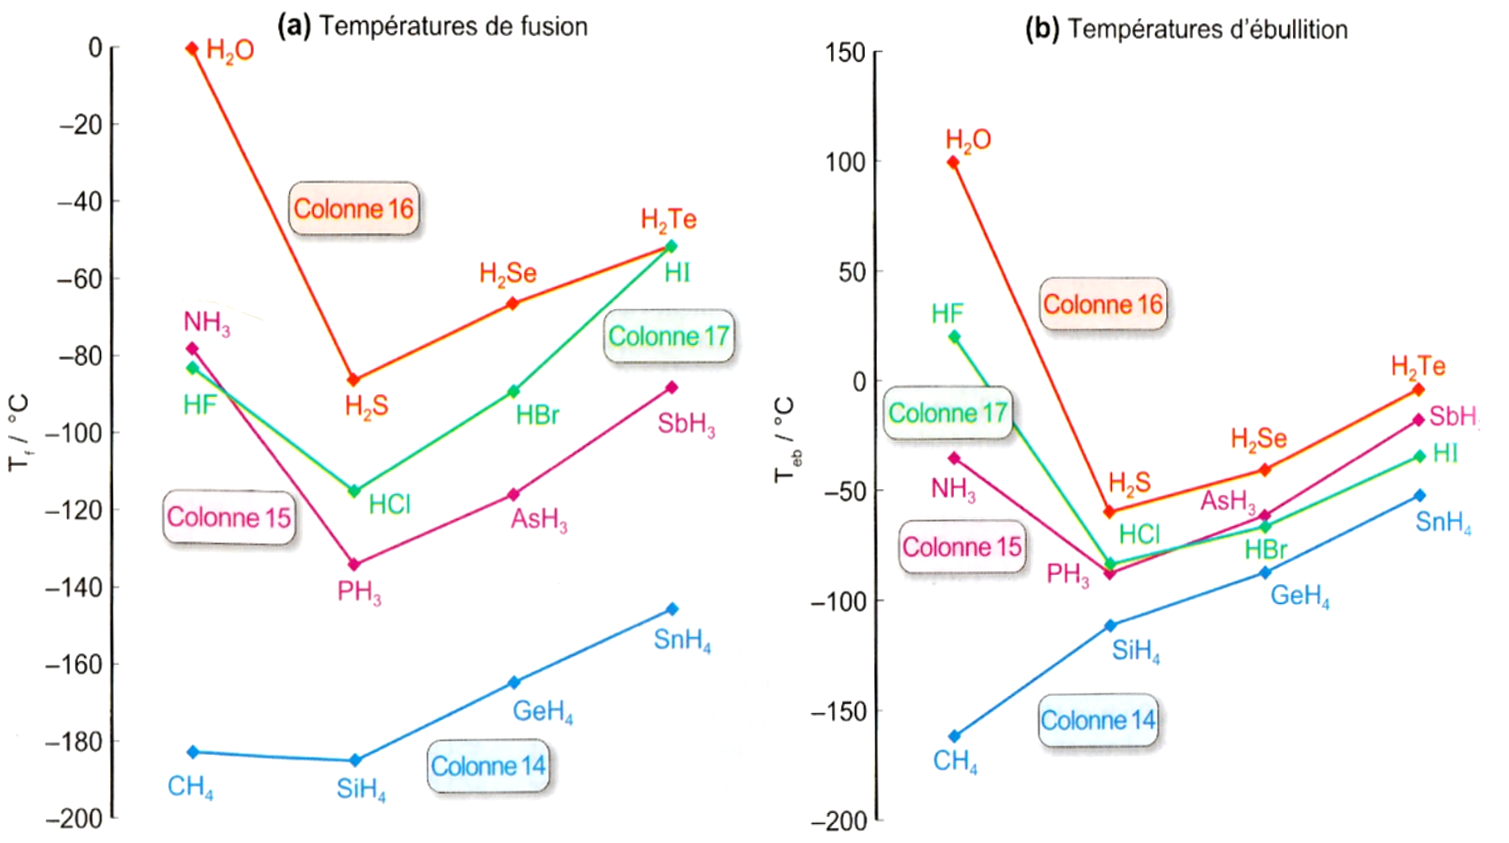
\includegraphics[width=.9\linewidth]{chimie/solvants/hydrures.png}
        \caption{Températures de fusion (a) et d'ébullition (b) des hydrures des éléments du bloc $p$ à pression atmosphérique.}
        \label{fig:hydrures}
    \end{figure}
\end{EnvUplevel}

\begin{table}[H]
    \centering
    \begin{tabularx}{.7\linewidth}{r|CCCC}
         & NH$_3$ & PH$_3$ & AsH$_3$ & SbH$_3$ \\ \hline\hline
        Solubilité vs H$_2$O (vol. / vol.) & 826 & 0,26 & 0,20 & 0,19 \\ \hline
    \end{tabularx}

    \caption{Comparaisons de propriétés chimiques des hydrures de pnictogènes (CTNP).}
    
    
\end{table}

\end{questions}

\end{exercise}

\begin{exercise}{Liasons moléculaires des nitrophénols}{2}{Sup}
{Liaisons chimiques}{bermu}

\begin{questions}

\questioncours Liaisons covalentes, liaisons hydrogène, liaisons Van der Waals. Analogies et différences. Comparaison des énergies associées.

\question En introduisant dans le détail les concepts utilisés, commenter l'évolution des caractéristiques physiques des différents nitrophénols : ortho, méta et para.
 
\begin{table}[H]  
	\setchemfig{chemfig style={scale=0.75}, atom style={scale=0.75}}
    \centering
    \begin{tabularx}{.8\linewidth}{r|CCC}
        & \chemfig{**6(---(-OH)-(-NO_3)---)}
        & \chemfig{**6(--(-OH)--(-NO_3)---)}
        & \chemfig{**6(-(-OH)---(-NO_3)---)}\\
%		& \chemfig[scale=0.75][scale=0.75]{**6(---(-OH)-(-NO_3)---)}
%       & \chemfig[scale=0.75][scale=0.75]{**6(--(-OH)--(-NO_3)---)}
%       & \chemfig[scale=0.75][scale=0.75]{**6(-(-OH)---(-NO_3)---)}\\
         & ortho & méta & para \\ \hline\hline
        Apparence & cristaux jaunes & cristaux incolores & aiguilles incolores \\
Point de fusion ($^\circ$C) & 44 & 97 & 114 \\
Point d'ébullition ($^\circ$C) & 214 & 194 & > 260 \\
pK$_a$ & 7,21 & 8,38 & 7,16 \\
Solubilité dans l'eau (g$\cdot$L$^{-1}$) & 2,1 & 13,5 & 14,8 \\ \hline
    \end{tabularx}

    \caption{Comparaisons de propriétés physiques des différents nitrophénols. (CTNP).}
\end{table}

\end{questions}

\end{exercise}

\section{Cristallochimie}
\begin{exercise}{Maille de l'argent}{1}{Sup}
{Cristalographie}{bermu}

L’argent cristallise dans un système cfc de paramètre $a = 408.6$ pm.

\begin{questions}
    \question Représenter schématiquement la maille de l'argent.
    \question Quelle est la valeur du rayon atomique de l’argent en supposant le cristal compact ?
\end{questions}
\end{exercise}

\begin{solution}
    \begin{questions}
        \question ~
        \question 
    \end{questions}
\end{solution}


%%%%%%%%%%%%%%%%%%%%%%%%%%%%%%%%%%%%%%%%%%%%%%%%%%%%%%%%%%%%%%%%%%%%%%%%%%%%%%%%%%%%%%%%%%%%%%%%%


\begin{exercise}{Variétés allotropiques du fer}{1}{Sup}
{Cristalographie,Variétés allotropiques}{bermu}

Le fer peut cristalliser suivant deux variétés allotropiques :
\begin{itemize}
    \item Fe$_\alpha$ : structure Cubique Centrée (CC), stable à basse température ;
    \item Fe$_\gamma$ : structure Cubique Faces Centrées (CFC), stable à haute température.
\end{itemize}

\noindent Pour chacune des deux structures :
\begin{questions}
    \question Représenter schématiquement la maille de chacun des deux réseaux.
    \question Préciser la coordinence et la population.
    \question Exprimer le rayon atomique du fer.
    \question Calculer la compacité de la structure ; lequel est le plus compact ?
    \question Exprimer la masse volumique des deux variétés.
\end{questions}

\paragraph{Données}
\begin{itemize}
    \item paramètre de maille du fer $\alpha$ : $a_\alpha = 291$ pm ;
    \item paramètre de maille du fer $\gamma$ : $a_\gamma = 365$ pm ;
    \item masse molaire du fer $M_\text{Fe} = 55,85~\mathrm{g\cdot mol^{-1}}$ ;
    \item nombre d'Avogadro $\cal{N}_\textsc{a} = 6,022\times 10^{23}~\mathrm{mol^{-1}}$ ;
\end{itemize}
\end{exercise}

\begin{solution}
    \begin{questions}
        \question ~
        \question (CC$\alpha$) Coordinence 8, Population 2 (CFC$\gamma$) Coordinence 12, Population 4
        \question (CC$\alpha$)$r_\alpha = \dfrac{\sqrt{3}}{4} a_\alpha = 126$ pm, (CFC$\gamma$)  $r_\gamma = \dfrac{\sqrt{2}}{4} a_\alpha = 129$ pm
        \question  (CC$\alpha$) 68\% (CFC$\gamma$) 74\%
        \question  (CC$\alpha$) 7530 $\mathrm{kg\cdot m^{-3}}$ (CFC$\gamma$) 7630 $\mathrm{kg\cdot m^{-3}}$
    \end{questions}
\end{solution}

%%%%%%%%%%%%%%%%%%%%%%%%%%%%%%%%%%%%%%%%%%%%%%%%%%%%%%%%%%%%%%%%%%%%%%%%%%%%%%%%%%%%%%%%%%%%%%%%%


\begin{exercise}{Stockage sous forme d'hydrures}{1}{Sup}
{Cristalographie,Alliages de substitution, Alliages d'insersion}{bermu}

Le dihydrogène peut être stocké dans les métaux sous forme d'hydrures métalliques. On étudie le processus de stockage
$$\mathrm{FeTi_{(s)} + \frac{\mathit{x}}{2} H_{2(g)} = FeTiH_{\mathit{x}(s)}},$$
$\mathit{x}$ étant un nombre stoechiométrique à déterminer.

L'alliage FeTi$_\mathrm{(s)}$ est une structure cubique simple comportant un atome de titane sur chaque sommet et un atome de fer au centre. Un atome d'hydrogène peut se placer dans les sites octaédriques de la maille métallique.

\begin{questions}
    \question Quel est le type d'alliage de FeTi ? Qu'en est-il lorsqu'il y a absorption d'hydrogène ?
    \question Représenter la maille de FeTi$_\mathrm{(s)}$ ainsi qu'un site octaédrique.
    \question Donner la population et la coordinence de chaque atome : Fe et Ti en l'absence d'hydrogène et H en supposant que tous les sites sont occupés. En déduire $\mathit{x}$.
    \question Donner le rayon d'habitabilité maximale du site intersticiel O. Est-ce cohérent avec les données ?
    \question En réalité, $\mathit{x} = 1,9$. Calculer la capacité volumique d'absorption de H$_2$ par FeTi en kg d'hydrogène par m$^3$ de FeTi.
\end{questions}

\paragraph{Données}
\begin{itemize}
    \item rayons atomiques : $r_\text{H} = 25$ pm / $r_\text{Fe} = r_\text{Ti} = 140$ pm ;
    \item paramètre de maille de FeTi $\gamma$ : $a = 298$ pm ;
    \item distance H--H dans H$_{2\text{(g)}}$ : $d_\text{H---H} = 74$ pm ;
    \item masse molaires (en $\mathrm{g\cdot mol^{-1}}$) : $\text{H} = 1,0$, $\text{Ti} = 47,9$, $\text{Fe} = 55,8$ ; 
    \item nombre d'Avogadro $\cal{N}_\textsc{a} = 6,022\times 10^{23}~\mathrm{mol^{-1}}$ ;
\end{itemize}
\end{exercise}

\begin{solution}
\begin{questions}
    \question Alliage de substitution pour FeTi avec insertion de H$_2$.
    \question ~
    \question Population : 1 Fe, 1 Ti, 3 H, Coordinences : Fe 8, Ti 8, H 4.
    \question $r = \dfrac{\sqrt{2}}{2}a - r_\text{Ti} = 71$ pm vs $r_\text{H} = 25$ pm et $d_\text{H---H} = 74$ pm.
    \question $\dfrac{\mathit{x} M_\text{H}}{\cal{N}_\textsc{a} a^3} = 112 \mathrm{kg\cdot m^{-3}}$.
\end{questions}
\end{solution}

%%%%%%%%%%%%%%%%%%%%%%%%%%%%%%%%%%%%%%%%%%%%%%%%%%%%%%%%%%%%%%%%%%%%%%%%%%%%%%%%%%%%%%%%%%%%%%%%%


\begin{exercise}{Semi-conducteurs}{1}{Sup}
{Cristalographie,Solides macrovalents}{bermu}

L'arséniure de gallium (AsGa) est un composé de la famille des semi-conducteurs III-V très utilisés en électronique. Sa structure est une maille cubique face centrée pour As avec occupation de 1 site tétraédrique sur 2 pour Ga.

\begin{questions}
    \question Représenter la maille de AsGa.
    \question Quelle est la population et la coordinence de la maille.
    \question Montrer que le rapport des rayons ioniques vérifie une condition que l'on donnera. Cela est-il cohérent avec la valeur du paramètre de maille ?
    \uplevel{L'AsGa est produit par épitaxie entre le gallium et le triiodure d'arsenic AsI$_3$ :
    $$\mathrm{2 Ga + 2 AsI_3 \longrightarrow 2 AsGa + 3 I_2}.$$
    }
    \question Quels types de solides sont ces espèces chimiques ?
\end{questions}

\paragraph{Données}
\begin{itemize}
    \item rayons ioniques : $r_\text{As} = 230$ pm, $r_\text{Ga} = 61$ pm ;
    \item paramètre de maille de AsGa $\gamma$ : $a = 565$ pm ;
    \item masse molaires (en $\mathrm{g\cdot mol^{-1}}$) : $\text{As} = 74.9$, $\text{Ga} = 69.7$ ; 
    \item nombre d'Avogadro $\cal{N}_\textsc{a} = 6,022\times 10^{23}~\mathrm{mol^{-1}}$ ;
\end{itemize}

\begin{figure}[H]
    \centering
    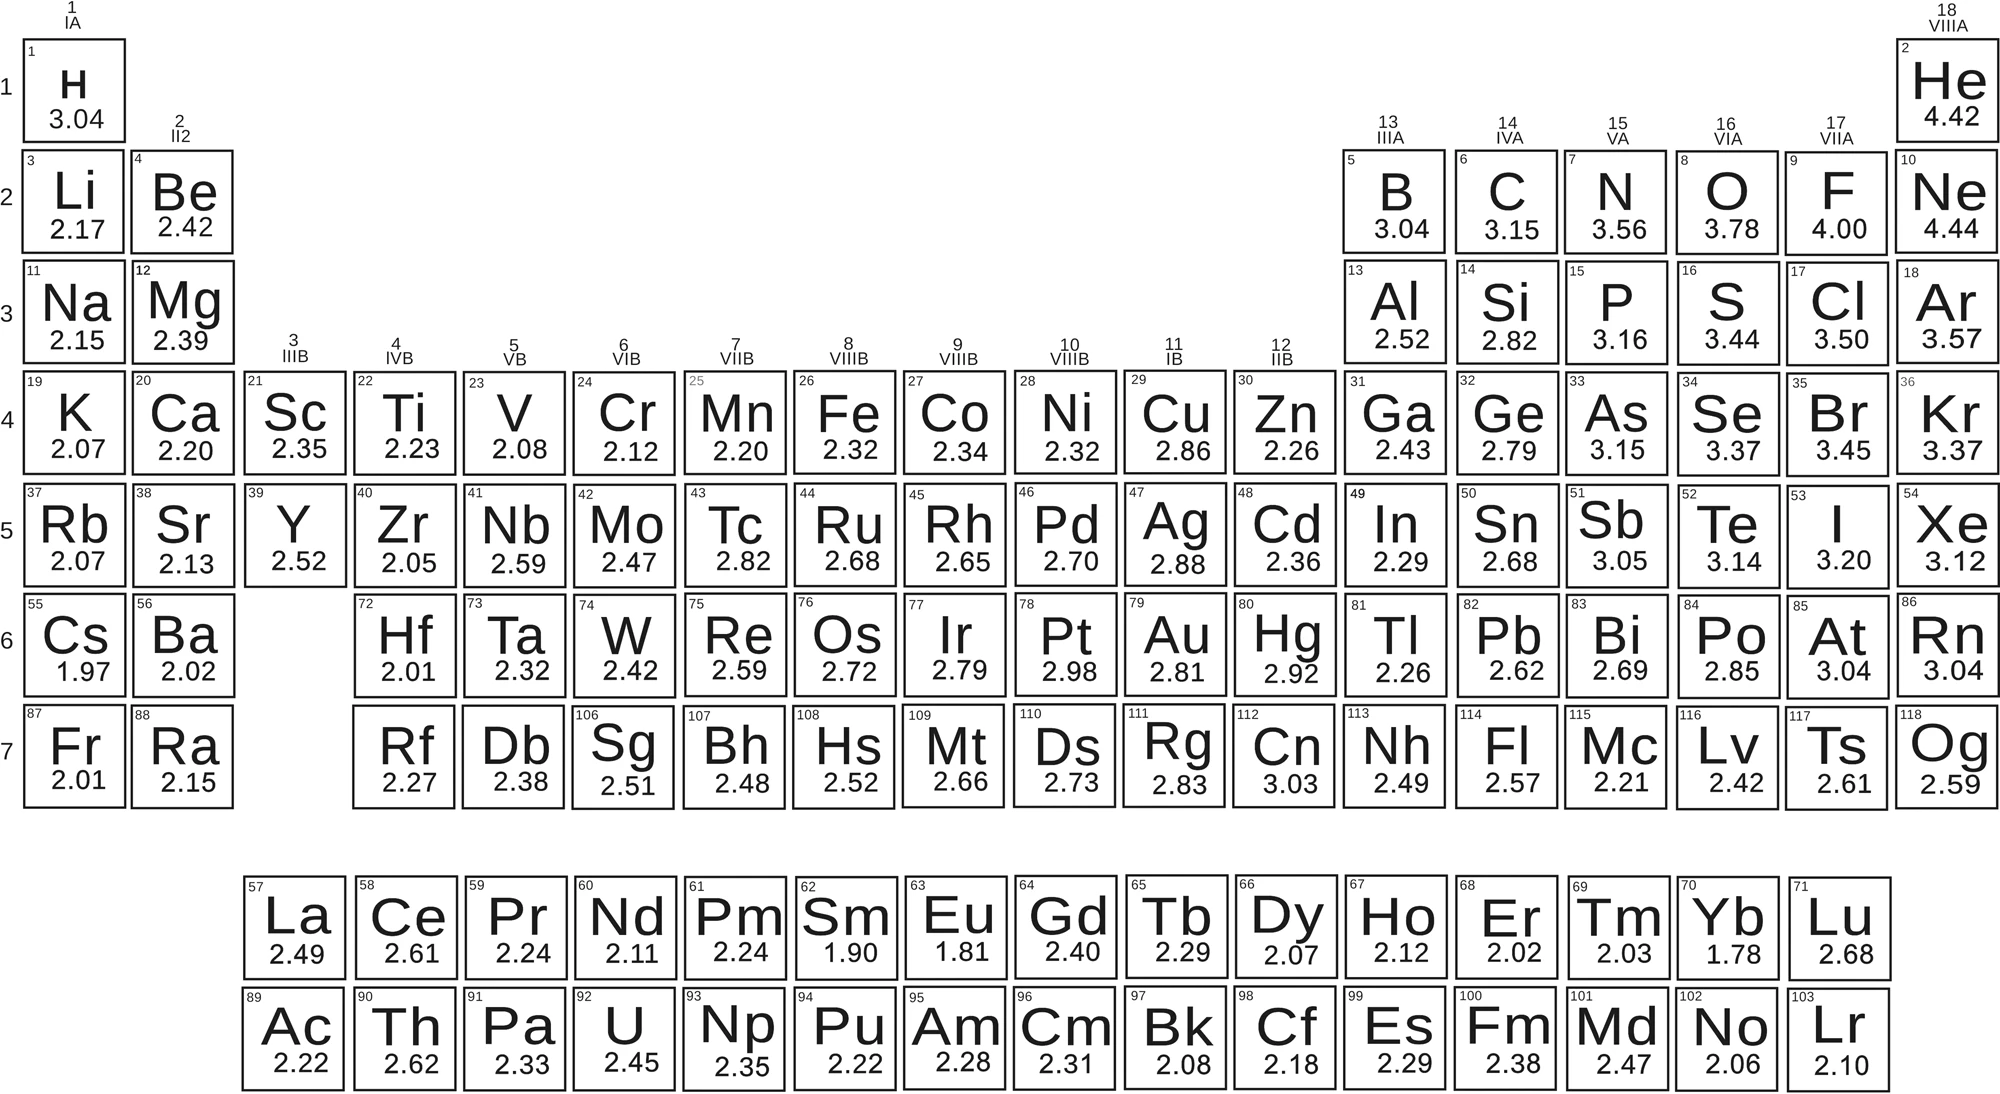
\includegraphics[width=\linewidth]{chimie/cristallo/electroneg_mulliken.png}
    \caption{Table périodique des électronégativités des éléments dans l'échelle de Mulliken.}
\end{figure}
\end{exercise}

\begin{solution}
\begin{questions}
    \question ~\\[0em] 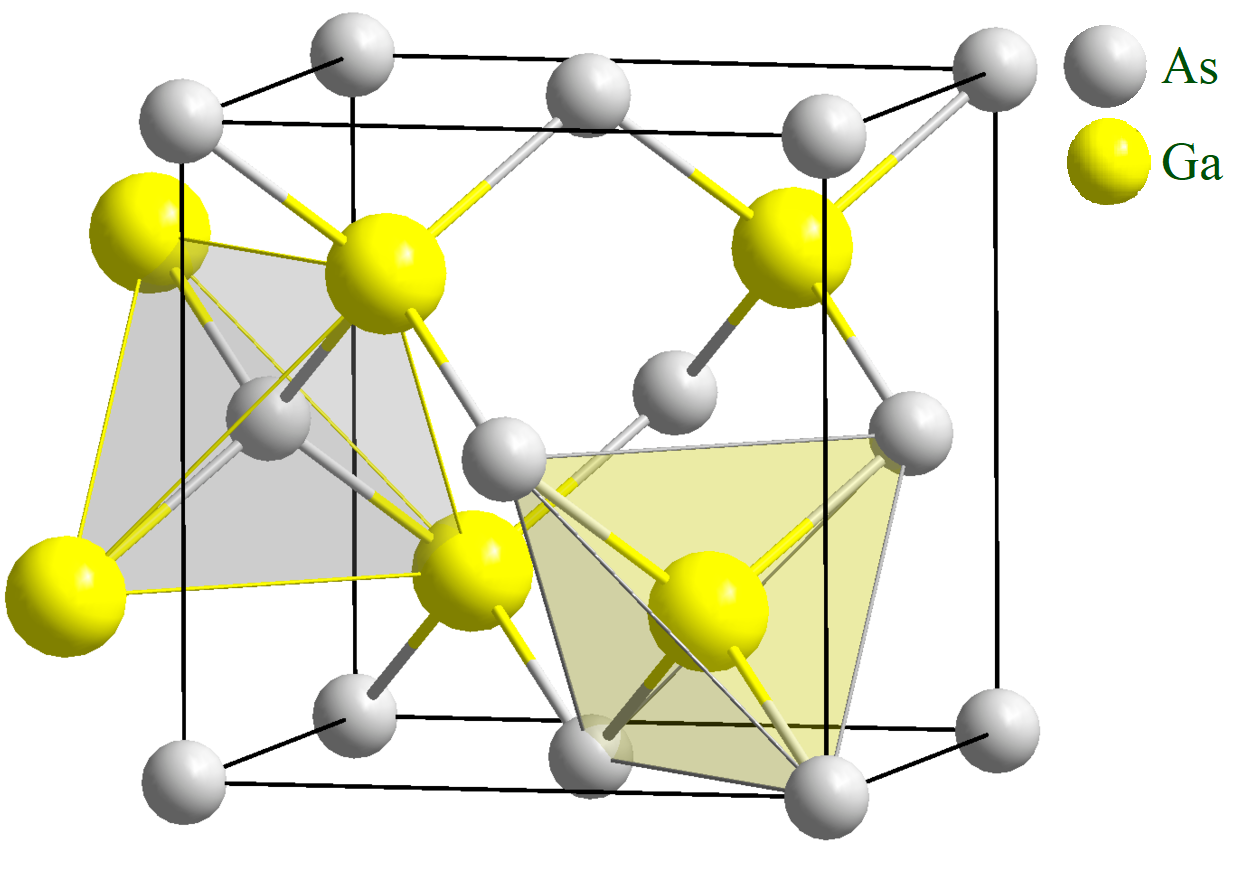
\includegraphics[width=0.45\linewidth]{chimie/cristallo/AsGa.png}
    \question Population 4 As $+$ 4 Ga, Coordinence 8 pour CFC, 4 pour As et Ga.
    \question $r_\text{Ga}/r_\text{As} > \sqrt{3/2} - 1 \simeq 0.225$.\\
    (\'Ealement $r_\text{Ga}/r_\text{As} < \sqrt{2}-1 \simeq 0.414$, l'autre maille étant NaC$\ell$, CFC insertion octaédrique)
    \question Ga : solide métallique, AsI$_3$ solide ionique, AsGa est un semi-métal, I$_2$ solide moléculaire
\end{questions}
\end{solution}

\section{\'Equilibres chimiques}
% Niveau :      PCSI *
% Discipline :  Chimie Orga
% Mots clés :   Stéréochimie

\begin{exercise}{Dimérisation du dioxyde d'azote}{2}{Sup,Spé}
{Transformationn de la matière,Equilibres chimiques}{bermu}

\begin{questions}
\questioncours Que signifie avoir atteint l'équilibre chimique ? En particulier, que cela signifie-t-il d'un point de vue des réactifs et des produits. \\
La réponse sera appuyée par des arguments de sens chimique et par un critère quantitatif.

\begin{EnvUplevel}
     Le dioxyde d'azote (NO$_2$, un gaz brun) a tendance suivant la température à se dimériser en péroxyde d'azote (N$_2$O$_4$, un gaz limpide). On note $K^\circ$ la constante de cet équilibre dans les conditions standard. 
     
     On suppose initialement que seule une quantité $c_0 = 1$ mol$\cdot$m$^{-3}$ de NO$_2$ est présente dans une enceinte à pression ambiante $P^\circ = 1$ bar et à température ambiante $T_1 = 300$ K.
     
     On introduit $\alpha$, l'avancement relatif comme étant le pourcentage (de volume) de N$_2$O$_4$ par rapport à NO$_2$.
\end{EnvUplevel}

\question \'Ecrire l'équilibre chimique entre NO$_2$ et N$_2$O$_4$, avec comme stoechiométrie 1 pour N$_2$O$_4$. \\
Qu'est-ce qui aurait changé si la stoechiométrie avait été différente ?

\question Exprimer le quotient réactionnel de la réaction $Q_r(\alpha)$ en fonction de $\alpha$ uniquement.

\question (\textsf{Application numérique}) $K^\circ(T_1) = 10^{-1}$. Calculer $\alpha_1$. \\
Justifier que le mélange gazeux soit brun.

\question On refroidit l'enceinte à $T_2 = 200$ K, toutes choses étant égales par ailleurs. Le mélange de gaz devient transparent. Comment évolue donc $K^\circ(T)$ avec $T$ ?

\uplevel{Pour quantifier les choses, il est mesuré avec un colorimètre l'absorption du gaz dans le brun aux températures $T_1$ et $T_2$.

L'absorption passe de $A_1 = 0.12$ à $A_2 = 0.02$.}

\question Trouver $\alpha_2$ et en déduire $K^\circ(T_2)$.


\end{questions}

\end{exercise}

% Niveau :      PCSI *
% Discipline :  Chimie Orga
% Mots clés :   Stéréochimie

\begin{exercise}{Du rose au bleu}{2}{Sup,Spé}
{Transformationn de la matière,Equilibres chimiques}{bermu}

\begin{questions}
\questioncours Critère d'évolution d'une réaction. \\
On introduira formellement toutes les notions présentées.

\begin{EnvUplevel}
     On étudie la réaction des ions cobalt (II) dans l'eau. Après un certain temps, le chlorure de cobalt (II) (CoC$l_4^{2-}$, bleu) réagissent avec l'eau pour former un complexe d'ion cobalt (II) entouré de molécules d'eau (Co(H$_2$O)$_6^{2-}$, rose).
     
     Initialement, on met $n_0 = 10$ mmol de chlorure de cobalt dans $V_0 = 200$ mL d'eau. Le mélange devient rose.
\end{EnvUplevel}

\question Avec ce que vous savez sur la molécule d'eau en tant que solvant, représenter dans l'espace le complexe Co(H$_2$O)$_6^{2-}$. Discuter le nombre de molécules d'eau liées à l'ion cobalt.

\question \'Ecrire l'équation de réaction avec une stoechiométrie 1 pour l'élément cobalt. On note $K^\circ$ la constante de réaction.

\question \'Ecrire le quotient de réaction en fonction de l'avancement $\xi$ (en mol), de $n_0$, de $V$, le volume de la solution et de $C^\circ$, la concentration standard.

\uplevel{On dilue peu a peu la solution, qui redevient bleu lorsque la solution a un volume $V_1 = 450$ mL de solution.}

\question Interpréter.

\question Au vue des observations, estimer $K^\circ$.

\question Quelle quantité de chlorure de sodium faut-il rajouter pour que la solution redevienne rose ?

\end{questions}

\end{exercise}

% Niveau :  PCSI *
% Discipline :  Chimie Orga
% Mots clés :   Stéréochimie

\begin{exercise}{Oxydation du cuivre par l'acide nitrique}{2}{Sup,Spé}
{Transformationn de la matière,Equilibres chimiques}{bermu}

\begin{questions}
\questioncours \'Ecriture de la loi d'action de masse pour différent systèmes. \\
On introduira formellement toutes les notions présentées.

\begin{EnvUplevel}
 On considère la réaction suivante d'oxydation du cuivre par l'acide nitrique :
 $$\mathrm{3 Cu_{(s)} + 8 H^+_{(aq)} + 2 {NO_3^-}_{(aq)} \quad\rightleftharpoons\quad 3 {Cu^{2+}}_{(aq)} + 2 NO_{(g)} + 4 H_20_{(\ell)}}, \qquad K^\circ = 10^{63}.$$
 
 À un instant donné, la solution, de volume $V_0 = 500$ mL, contient 30 mM d’ions Cu$^{2+}$, 80 mM d'ions nitrate NO$_3^-$, et un pH$ = 1$ (pour rappel pH = -log[H$^+$]). Un morceau de cuivre de $m = 12$ g est immergé dans  la solution ($M_\text{Cu} = 63,5$ g$\cdot$mol$^{-1}$). La solution est surmontée d’une atmosphère fermée de volume $V_\text{g} = 1,0$ L où la pression partielle en monoxyde d’azote est $p_\text{NO} = 15$ kPa.
\end{EnvUplevel}

    \question Le système est-il à l'équilibre ?
 
    \question Décrire précisément l’état final du système. \\
 Comment peut on qualifier l'état final (deux réponses attendues).
 
 \uplevel{On refait le protocole avec $m = 1$ g de cuivre.}
 
    \question Refaire la question précédente.
 
    \question En deçà de quelle masse le cuivre est-il limitant ?
 
 
 

\end{questions}


\end{exercise}

\begin{solution}

H$^+$ est limitant. $\xi_\text{max} = 6,25$ mmol. $\epsilon = 4.1\times 10^{-9}$ mol. pH = 8.1.

\end{solution}

\section{Réactions acide-base}
\begin{exercise}{Glycine}{1}{PCSI}
{Acides et bases,Equilibres chimiques}{lelay}

La glycine (ou glycocolle) est un acide aminé de structure H$_2$N--CH$_2$--COOH.  C'est un ampholyte : en effet, dans l'eau, la glycine est engagée dans deux couples acido-basiques de $\text{p}K_\text{a}$ 2.4 et 9.6.

\begin{questions}
    \question Dans l'eau, la glycite est un zwitterion (ou amphion), c'est à dire qu'elle possède à la fois une charge positive et une charge négative. Donner la représentation de Lewis de la glycine dans l'eau.

    \question Écrire les équilibres acido-basiques faisant intervenir la glycine dans l'eau.

    \question Tracer le diagramme de prédominance des espèces de la glycine en fonction du pH de la solution

    \question En solution neutre, quelle est l'espèce majoritaire ?
    
    \question Quel est le pH approché d'une solution de glycine à 10$^{-1}$~M ?
    
    \question L'électrophorèse est une technique permettant de faire migrer les ions d’une solution, sur un support solide, sous l’action d’un champ électrique. À quel pH faut-il opérer l’électrophorèse d’une solution de glycocolle de concentration 10$^{-1}$~M pour que 99\% des ions migrent vers le pôle positif ?
    
\end{questions}
\end{exercise}

\begin{solution}
\begin{questions}

    \question ion glycinium NH$_3^+$ COOH et ion glycinate NH$_2$ COO$^-$
    
    \question ion glycinium - pH 2.4 - glycine - pH 9.6 - ion glycinate
    
    \question À pH = 7 c'est la glycine, l'amphion.
    
    \question On part d'une concentration $C_0 = 0.1$~mol/L en glycine qui réagit selon 2~glycine~=~glycinium~+~glycinate (réaction prépondérante en solution neutre).
    
    On a $K = Ka_2 / Ka_1 = 10^{-7.2}$ c'est bien l'équilibre de contrôle.
    
    Donc d'après le tableau d'avancement [glycinium] = [glycinate] = $x$ et il se trouve que [H$^+$]$^2$ = $Ka_1 \, Ka_2$ d'où $pH = \frac12(pKa_1 + pKa_2) = 6.2$.
    
    \question On veut [glycinate] = 0.99 $c_0$, on ne prend en compte que l'équilibre glycine - glycinate car l'autre est negligeable. 
    
    On utilise la relation de Henderson : $pH = pKa_2 + log([glycinate][glycine]) = 10.6$.
    
\end{questions}
\end{solution}

%%%%%%%%%%%%%%%%%%%%%%%%%%%%%%%%%%%%%%%%%%%%%%%%%%%%%%%%%%%%%%%%%%%%%%%%%%%%%%%%%%%%%%%%%%%%%%%%%%%%%%%%%%%%%%

\begin{exercise}{Imidazole}{1}{PCSI}
{Acides et bases,Equilibres chimiques}{lelay}

L’imidazole, que l’on notera L pour simplifier est une molécule organique de formule C$_3$N$_2$H$_4$. En solution aqueuse, l’imidazole L se comporte comme une monobase faible, le couple LH$^+$/L ayant un $pK_a$ égal à 6.95.

\begin{questions}

    \question On dispose de 50~mL d'une solution acqueuse d'imidazole de concentration 0.02~mol/L. Quel est le pH de cette solution ?

    \question On ajoute à la solution précédente un volume $V$ d’une solution aqueuse d’acide chlorhydrique de concentration 0,50 mol.L$^{-1}$. Calculer, de manière simplifiée, le pH de la solution obtenue correspondant aux valeurs suivantes de $V$ : 0,5 ; 1,0 ; 1,5 ; 2,0 et 2,5 mL.

    \question Représenter l'allure de la courbe $pH = f(V)$
    
\end{questions}
\end{exercise}

\begin{solution}
\begin{questions}

    \question Reaction L = LH+ + HO-, en la supposant peu avancée $K = x^2 / C_0$, on en déduit 
    $$ pH = \frac12\qty( pK_e + pK_a +\log C_0) = 9.6 $$. On a bien pH > pKa + 1 donc L ets majoritaire et pH > 7.5 donc l'autoprotolyse de l'eau est négligeable.
    
    \question La réaction prépondérante est H+ + L = LH+ de constante 10$^{6.95}$ $\gg 1$ donc quantitative.
    \begin{itemize}
        \item Pour V= 0.5, 1.0 et 1.5 mL, on applique juste henderson en supposant que la réaction est totale et pH = 7.4, 6.95, 6.5
        \item Pour V = 2.0 mL tout l'acide a été consommé, la solution est équivalent a une solution d'acide faible LH+ dans 52 mL de solution, d'où $pH = \frac12(pK_a - \log C) = 4.3$
        
        \item Pour V = 2.5 mL on a un excès de 0.25 mmol de H+ pour 52.5 mL de solution. C'est un mélange d'acide faible et d'acide fort. L'acide fort impose le pH d'où $pH = -log [H30+] = 2.3$
    \end{itemize}
    
    \question Typique titrage de baise faible par acide fort.
    
\end{questions}
\end{solution}

%%%%%%%%%%%%%%%%%%%%%%%%%%%%%%%%%%%%%%%%%%%%%%%%%%%%%%%%%%%%%%%%%%%%%%%%%%%%%%%%%%%%%%%%%%%%%%%%%%%%%%%%%%%%%%

\begin{exercise}{Pluies acides}{1}{Sup}
{Acides et bases,Equilibres chimiques}{bermu}

L’eau de pluie est naturellement acide (pH voisin de 6), en raison du dioxyde de carbone qu’elle
dissout. Cette acidification est très nettement augmentée dans les zones à forte activité industrielle. La
pollution par les oxydes de soufre constitue l’une des hypothèses avancées pour expliquer ce
phénomène.

Pour modéliser l’effet de SO$_2$ sur l’acidité de l’eau, on place de l’eau initialement pure dans un récipient
à l’intérieur duquel est maintenue une pression constante de dioxyde de soufre gazeux égale à $\SI{8e-8}{bar}$ à $T = \SI{298}{K}$.

Pour la commodité des calculs, on considère comme négligeable la concentration de SO$_{2\text{(aq)}}$.

\begin{questions}

    \question Tracer le diagramme de prédominance des espèces acido-basiques du soufre intervenant dans la
solution aqueuse.

    \question Sachant que la solution à l’équilibre est plus acide que l’eau de pluie naturelle, quelle espèce du
diagramme de prédominance précédent est assurément en concentration négligeable ?

    \question En déduire l’équation chimique responsable majoritairement de l’acidification de l’eau.

    \question Calculer alors le pH de la solution
    
    \plusloin Vérifier l’hypothèse formulée en \textsfbf{Q2}.
    
\end{questions}

\paragraph{Données :}
$$\text{p}K_\text{a1}(\mathrm{H_2SO_3/HSO_3^-}) = 1,8  \qquad \text{p}K_\text{a2}(\mathrm{HSO_3^-/SO_{3}^{2-}}) = 7,2.$$
Dissolution de SO$_{2\text{(g)}}$ :

$$\mathrm{SO_{2(g)} + H_2O \longrightarrow H_2SO_3} \qquad K_\textsc{h} = \SI{1,25}{}$$

\end{exercise}

\begin{solution}
\begin{questions}

    \question $\mathrm{H_2SO_3/HSO_3^-/SO_{2}}$
    
    \question $\mathrm{SO_{3}^{2-}}$ négligeable

    \question $\mathrm{SO_{2(g)} + 2 H_2O \longrightarrow HSO_3^- + H_3O^+} \qquad K^\circ = K_\textsc{h} 10^{-\text{p}K_\text{a1}} = 0.02$
    
    \question $K^\circ = \dfrac{\mathrm{[H_3O^+][HSO_3^{-}]}}{P_\mathrm{SO_2}}$ or $\mathrm{[H_3O^+] = [HSO_3^{-}] = 10^{-pH}}$

    $\text{pH} = 4.4$.
    
\end{questions}
\end{solution}
% Niveau :      PCSI *
% Discipline :  Chimie Orga I
% Mots clés :   Spectrométrie UV-visible, Réactions acidobasiques

\begin{exercise}{Bleu de bromothymol}{2}{PCSI}
{Chimie générale,Réactions acidobasiques,Spectroscopie,UV-visible}{bermu}


Le bleu de bromothymol (BBT) est un indicateur de pH très utilisé en biologie pour mettre en évidence la présence de $\mathrm{CO_2}$. Vers $\text{pH} = 7.1$, il passe de sa forme acide jaune à sa forme basique bleue (notées $\mathrm{InH}$ et $\mathrm{In^{-}}$ respectivement) :\vspace{-.5em}
\begin{center}
        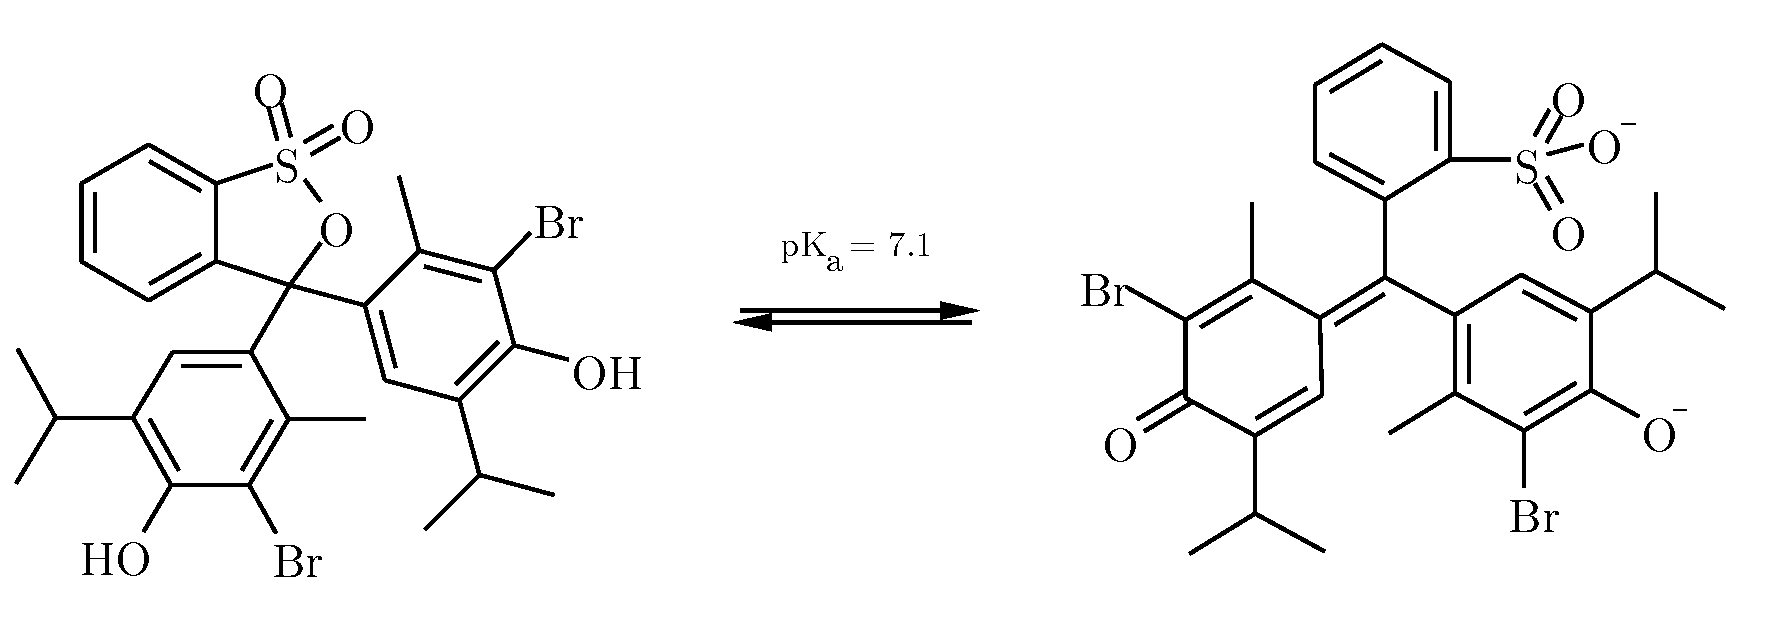
\includegraphics[width=.7\linewidth]{chimie/pH/BBT1.pdf}.\vspace{-1.5em}
\end{center}

\begin{questions}
\questioncours Théorie de Brönsted des acides et des bases. On précisera la définition du pK$_a$ et du pK$_e$.

\question Tracer le diagramme de prédominance de InH / In$^-$ en précisant la couleur de la solution dans chaque cas. Comparer à quelques exemples de couples acidobasiques connus.

\question Le CO$_2$ se comporte comme un diacide de pK$_a$ 6,4 et 10,3. \\ Tracer le diagramme de prédominance de CO$_2$ et discuter de l'utilisation du BBT pour la mise en évidence du CO$_2$ \textit{in vivo}.

\question\label{qu:1} Donner la relation entre le pH et le taux de dissociation $\alpha = \dfrac{\mathrm{[In^-]}}{\mathrm{[InH] + [In^-]}}$ du BBT.

\begin{EnvUplevel}
   On propose une méthodologie pour mesurer le pH d'une cellule par mesure de l'absorbance à l'aide du BBT :
    \begin{figure}[H]
        \centering
        \begin{tabularx}{\linewidth}{XX}
            \small{\textbf{(a)}} & \small{\textbf{(b)}}. \\
            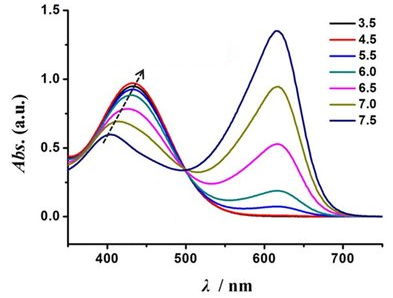
\includegraphics[width=\linewidth]{chimie/pH/BBT2.png} &
            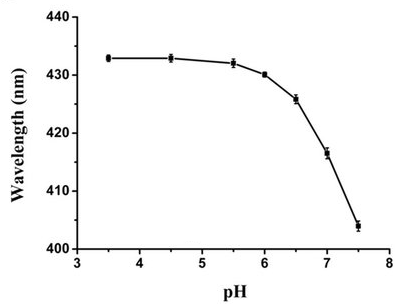
\includegraphics[width=\linewidth]{chimie/pH/BBT3.png}
        \end{tabularx}\vspace{-.5em}
        \caption{Spectres d'absorption UV-Visible (\textbf{a}) et courbe de calibration du pic à $\sim$ 420 nm (\textbf{b}) du bleu de bromothymol (BBT) pour différentes valeurs de pH. (Hui Hou, \emph{Nature Scientific Reports}, 7:1759, 2017)}
        \label{fig:BBT2}
    \end{figure}
\end{EnvUplevel}\vspace{-2ex}

\question Énoncer la loi de Beer--Lambert en précisant les hypothèses de validité.

\question Interpréter qualitativement la Fig.~(\textbf{a}) avec les deux maxima $\lambda_\text{max,a} = 433$ nm et {$\lambda_\text{max,b} = 616$~nm}.

\question\label{qu:2} Rappeler l'intérêt de mesurer l'absorbance au niveau des maxima d'intensité et justifier sans calcul que pour une seule espèce $i$
$$A_i(\lambda) \simeq A_{i,\text{max}}\,\qty(1 - \kappa_i\,\qty(\lambda - \lambda_{i,\text{max}})^2) \qqtext{pour} \lambda \simeq \lambda_{i,\text{max}},$$
$\kappa_i$ étant une constante qui dépend du chromophore à $\lambda_{i,\text{max}}$.

%\question Le point $\lambda_i = 500$ nm est nommé un point isobestique. Justifier par un simple calcul que ce point d'absorption constante $A_i$ durant la transformation $\mathrm{InH \xrightleftharpoons{} In^- + H^+}$ indique que cette transformation ne fait pas intervenir d'intermédiaire. \vspace{-2em}
%\begin{EnvUplevel}
%\paragraph{Indication :} exprimer l'absorbance de la solution en fonction des concentrations $[\mathrm{In^-}]$ et $[\mathrm{InH}]$.

%On va maintenant s'intéresser à modéliser la courbe de calibration.
%\end{EnvUplevel}

\question La forme basique du BBT possède également un maximum d'absorption en $\lambda_\text{max,b'} = 403$~nm. \\ A l'aide de la question \ref{qu:2}, donner l'absorption totale de la solution $A_\text{tot}$ en fonction de $\alpha$.

\question Donner longueur d'onde d'absorption maximale $\lambda_\text{max}$ en fonction de $\alpha$. Est-ce cohérent avec la Fig. (\textbf{b}) ?

%\question \`A l'aide de la relation d'Henderson--Hasselbalch et du $\mathrm{pK_a}$ du BBT, exprimer la relation $\lambda(\text{pH})$. \\

\end{questions}
\end{exercise}

\begin{solution}
\begin{questions}
    \questioncours
    \begin{itemize}
        \item Un acide de Brönsted est un donneur de H$^+$, une base de Brönsted est un accepteur de H$^+$ ;
        \item Le $K_a$ est la constante d'équilibre de la réaction
        \begin{center}\schemestart
        AH
        \arrow{<=>}[,1]
        A$^-$
        \+
        H$^+$
        \schemestop\chemnameinit{},\end{center}
        dont on déduit la relation de Henderson--Hasselbalch
        $$K_a = \mathrm{\dfrac{[A^-][H^+]}{[AH]}} \quad \Longleftrightarrow \quad \text{p}K_a = -\log K_a = \text{pH} + \log\mathrm{\dfrac{[A^-]}{[AH]}}.$$
        \item Le $K_e = 10^{-14}$ à 25$^\circ$C est la constante d'équilibre de la réaction d'autoprotolyse de l'eau
        \begin{center}\schemestart
        H$_2$O
        \arrow{<=>}[,1]
        H$^+$
        \+
        HO$^-$
        \schemestop\chemnameinit{},\end{center}
        dont on déduit la relation du produit ionique de l'eau
        $$K_e = \mathrm{[H^+][OH^-]}.$$
    \end{itemize}
    
    \question \hfill 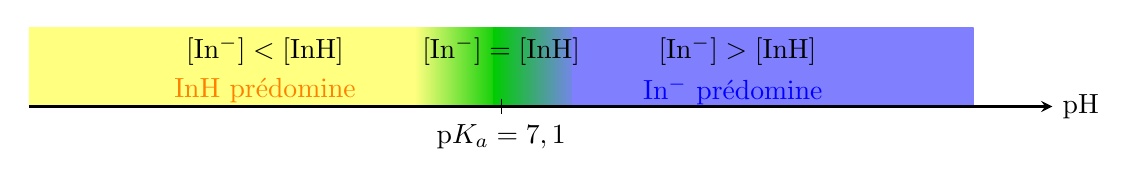
\begin{tikzpicture}[baseline=1em]
        \shade[left color = yellow!50, right color = yellow!50] (-6,0)rectangle(-1,1) ;
        \shade[left color = yellow!50, right color = green!80!black] (-1.1,0)rectangle(0,1) ;
        \shade[right color = blue!50, left color = green!80!black] (-.1,0)rectangle(1,1) ;
        \shade[right color = blue!50, left color =blue!50]
        (.9,0)rectangle(6,1) ;
        \node at (-3,.2) {\textcolor{orange}{InH prédomine}};
        \node at (3,.2) {\textcolor{blue}{$\mathrm{In^-}$ prédomine }};
        \draw[->, >=stealth, thick] (-6,0)--(7,0) node[right]{pH};
        \draw[black] (0,0.1)--(0,-0.1) node[below]{$\mathrm{p}K_a = 7,1$} ;
        \node at (-3,.7){$\left[ \mathrm{In^-}\right] < \left[ \mathrm{InH}\right]$};
        \node at (0,.7){$\left[ \mathrm{In^-}\right] = \left[ \mathrm{InH}\right]$};
        \node at (3,.7){$\left[ \mathrm{In^-}\right] > \left[ \mathrm{InH}\right]$};
    \end{tikzpicture} \hfill ~
    \newcommand{\tik}[4]{%
        \node[above] at (#1,.1){$\mathrm{#3}$};
        \node[above] at (#1,.9){$\mathrm{#4}$};
        \draw[black] (#1,0.1)--(#1,-0.1) node[below]{#2};
    }
    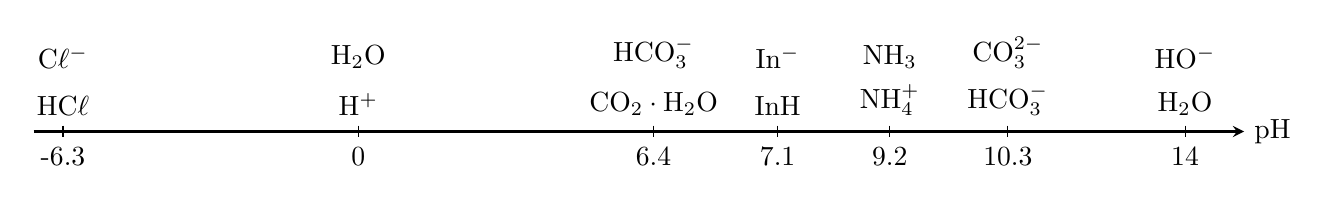
\begin{tikzpicture}[baseline=1em, scale=0.75]
        \draw[->, >=stealth, thick] (-5.5,0)--(15,0) node[right]{pH};
        \tik{-5}{-6.3}{HC\ell}{C\ell^-}
        \tik{0}{0}{H^+}{H_2O}
        \tik{14}{14}{H_2O}{HO^-}
        \tik{7.1}{7.1}{InH}{In^-}
        \tik{5}{6.4}{CO_2\cdot H_2O}{HCO_3^-}
        \tik{11}{10.3}{HCO_3^-}{CO_3^{2-}}
        \tik{9}{9.2}{NH_4^+}{NH_3}
    \end{tikzpicture}
    
    \question D'après la relation d'Henderson--Hasselbalch
    $$\text{p}K_a = \text{pH} + \log\mathrm{\dfrac{[In^-]}{[InH]}}
    = \text{pH} + \log\mathrm{\dfrac{[In^-]}{[In^-] + [InH]} \times \dfrac{[In^-] + [InH]}{[InH]}} = \text{pH} + \log\dfrac{\alpha}{1 - \alpha}.$$
    
    \question cf. \textbf{\sffamily Q2}. Le BBT devient jaune dès que le pH est inférieur à $\sim$ 7.1, or lorsqu'on dissout du CO$_2$, le pH baisse en dessous de 7, donc le BBT un indicateur adapté à cet usage.
    
    \question Pour des concentrations entre $10^{-3}$ M et $10^{-1}$ M, on a
    $$A(\lambda) = \ell\sum_i \varepsilon_i(\lambda) c_i,$$
    $A$ étant l'absorption de la solution, \\
    $\ell$ la taille de la cuve, \\
    $\varepsilon_i$ le coefficient d'absorption molaire du chromophore $i$, \\
    $c_i$ la concentration du composé $i$.
    
    \question La mesure au maximum d'absorption permet de minimiser l'erreur car $\Delta A \propto \Delta\lambda^2$ et de maximiser le signal par rapport au bruit.
    
    Pour $\lambda = \lambda_{i,\text{max}}$, $A_i = A_{i,\text{max}}$, et l'absorption diminue si on s'éloigne de $\lambda_{i,\text{max}}$ quadratiquement car on est à un max. 
    
    \question On remarque que la forme acide a un maximum d'absorption à $\lambda_\text{max,a} = 433$ nm dans le bleu (jaune en transmission), et la forme basique a un maximum d'absorption à $\lambda_\text{max,b} = 616$ nm dans le orange (bleu en transmission), ce qui est cohérent avec la couleur du BBT.
    
    \question $A_\text{tot} = \alpha A_{\text{max,b}}\,\qty(1 - \kappa_b\,\qty(\lambda - \lambda_{\text{max,b}})^2) + (1-\alpha) A_{\text{max,a}}\,\qty(1 - \kappa_a\,\qty(\lambda - \lambda_{\text{max,a}})^2)$
    
    \question $\displaystyle\eval{\pdv{A_\text{tot}}{\lambda}}_{\lambda_\text{max}} = 0 = 
    2\lambda_\text{max}\qty\bigg[\qty\Big(\gamma_a \lambda_\text{max,a} + \alpha (\gamma_b \lambda_\text{max,b} - \gamma_a \lambda_\text{max,a})) - \lambda_\text{max} \qty\Big(\gamma_a + \alpha(\gamma_b - \gamma_a))]$
    où  $\gamma_i = \kappa_i \varepsilon_i$
    $$\text{d'où}\qquad \lambda_\text{max} = \dfrac{\gamma_a \lambda_\text{max,a} + \alpha (\gamma_b \lambda_\text{max,b} - \gamma_a \lambda_\text{max,a})}{\gamma_a + \alpha(\gamma_b - \gamma_a)}
        = \lambda_\text{max,a} + \alpha \dfrac{\lambda_\text{max,b} - \lambda_\text{max,a}}{\gamma_a/\gamma_b + \alpha(1 - \gamma_a/\gamma_b)}$$
    ce qui est cohérent avec la figure b.
\end{questions}
\end{solution}
% Niveau :      PCSI *
% Discipline :  Chimie Orga I
% Mots clés :   Spectrométrie UV-visible, Réactions acidobasiques

\begin{exercise}{Autour de la loi d'Ostwald}{2}{PCSI}
{Chimie générale,Réactions acidobasiques,Loi d'Ostwald}{bermu}

\begin{questions}
\questioncours Définir acide fort, acide faible, base forte et base faible. \\
On donnera un exemple d’espèce chimique pour chacune de ces catégories.

\begin{EnvUplevel}
    Nous allons  par la suite étudier les effets de la dilution de l'acide propanoïque, noté AH, de p$K_\text{a}= 4,9$.

    On dilue dans un volume $V$ d'eau déionisée une quantité initiale $n$ de AH solide et on note
    $$c = \dfrac{n}{V C^\circ} \qqtext{et} \text{p}c = -\log c,$$
    avec $C^\circ = 1$~mol$\cdot\text{L}^{-1}$ (la variation de volume est négligée).
\end{EnvUplevel}
\question Donner la formule de AH. Quel genre d'acide est-ce ?

\question\label{qu:osw} Donner une estimation rapide du pH de la solution en fonction de p$c$ et énoncer la loi d'Ostwald.

\uplevel{Nous allons désormais calculer plus rigoureusement le pH de cette solution.}

\question \'Ecrire le tableau d'avancement de la réaction acidobasique avec le coefficient de dissociation
$$\alpha = \dfrac{\mathrm{[A^-]}}{\mathrm{[AH] + [A^-]}}.$$

\question\label{qu:alpha} Déduire en fonction de p$c$, p$K_\text{a}$ et p$K_\text{e} = 14$ l'équation du second degré vérifiée par $\alpha$.
%$$\alpha = \dfrac{10^{\text{p}c - \text{p}K_\text{a}}}{2}\qty(\sqrt{(1 + 10^{\text{p}K_\text{a} - \text{p}K_\text{e}/2})^2 + 10^{-(\text{p}c - \text{p}K_\text{a})}} - (1 + 10^{\text{p}K_\text{a} - \text{p}K_\text{e}/2}))$$

\question Quel autre réaction n'est pas prise en compte ? Comment la prendre en compte ?

\begin{EnvUplevel}
    Dans le cas le plus général, la pH de la solution évolue comme suit : \vspace{-1em}
    \begin{figure}[H]
        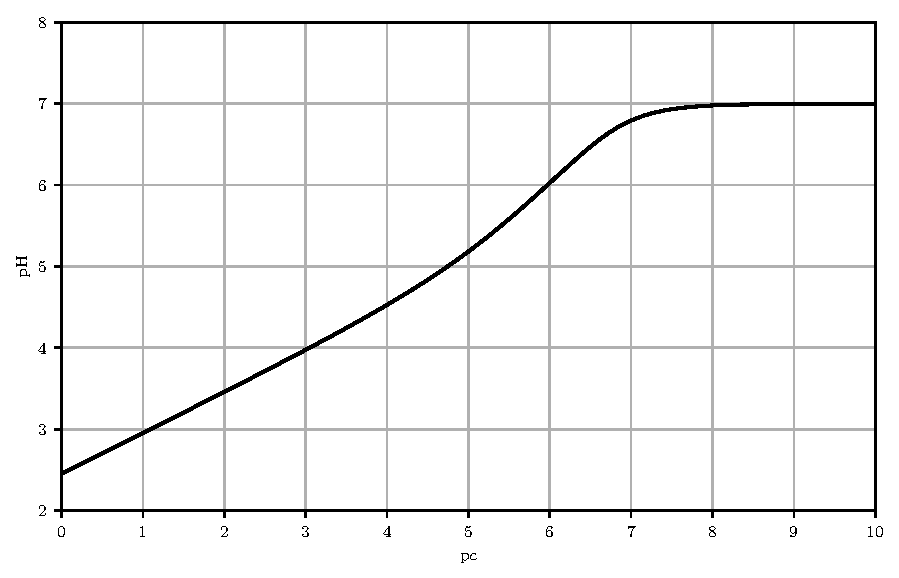
\includegraphics[width=\linewidth]{chimie/pH/ostwald.pdf}\vspace{-.8em}
        \caption{pH et taux de dissociation $\alpha$ de la solution en fonction de p$c$.}
    \end{figure}
\end{EnvUplevel}

\question \`A l'aide des questions \ref{qu:osw} et \ref{qu:alpha}, étudier et interpréter les cas :

~\hfill \textbf{\sffamily a)} $\text{p}c \ll \text{p}K_\text{a}$ \hfill 
\textbf{\sffamily b)} $\text{p}K_\text{a} \ll \text{p}c \ll \text{p}K_\text{e}/2$ \hfill
\textbf{\sffamily c)} $ \text{p}K_\text{e}/2 \ll \text{p}c$. \hfill ~

\question Justifier l'affirmation : \textsl{pour de hautes dilutions, un acide faible a un comportement d'acide fort}.

\end{questions}
\end{exercise}

\begin{solution}
\begin{questions}
    \questioncours
    \begin{center}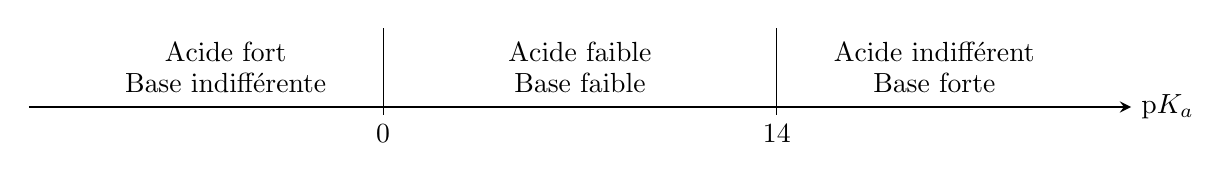
\begin{tikzpicture}[baseline=1em]
        \draw[->, >=stealth, thick] (-7,0)--(7,0) node[right]{p$K_a$};
        \draw[black] (-2.5,1)--(-2.5,-0.1) node[below]{0} ;
        \draw[black] (2.5,1)--(2.5,-0.1) node[below]{14} ;
        \node at (-4.5,.3) {Base indifférente};
        \node at (0,.3) {Base faible};
        \node at (4.5,.3) {Base forte};
        \node at (-4.5,.7) {Acide fort};
        \node at (0,.7) {Acide faible};
        \node at (4.5,.7) {Acide indifférent};
    \end{tikzpicture}\end{center}
    
    \question $\mathrm{AH \equiv CH_3\text{--}CH_2\text{--}COOH}$, c'est un acide faible.
    
    \question Pour un acide faible, $\text{pH} = \dfrac{1}{2}\qty(\text{p}K_a + \text{p}c)$. Plus on dilue l'acide, et plus il est dissocié.
    
    \question ~ \\[-2.5em]
    \begin{center}\begin{tabularx}{10cm}{r|C|C|C}
&
\multicolumn{1}{|c!{\makebox[0pt]{$\leftrightharpoons$}}}{AH}
&
\multicolumn{1}{c!{\makebox[0pt]{+}}}{A$^-$}
&
H$^+$
\\
\hline\hline
Init. & $c$ & 0 & $10^{-\text{p}K_e/2}$ \\
Eq. & $(1-\alpha)c$ & $\alpha c$ & $10^{-\text{p}K_e/2} + \alpha c$
\end{tabularx}\end{center}
    
    \question\hfill $10^{-\text{p}K_a} = \mathrm{\dfrac{[A^-][H^+]}{[AH]}} = \dfrac{\alpha\qty(10^{-\text{p}K_e/2} + \alpha 10^{-\text{p}c})}{1 - \alpha},$ \hfill ~
    $$\text{d'où}\qquad \alpha^2 + \alpha\qty(10^{\text{p}c - \text{p}K_a} + 10^{\text{p}c - \text{p}K_e/2}) - 10^{\text{p}c-\text{p}K_a} = 0. \qquad (\ast)$$
    
    \question On n'a pas pris en compte l'autoprotoloyse de l'eau. Pour la prendre en compte, il faudrait ajouter un second avancement $\beta$ permettant d'établir deux équations à deux inconnues $\alpha, \beta$.
    
    \question Pour cet acide faible, on a p$K_a \ll \text{p}K_e/2$.
    
    \textbf{\sffamily a)} Dans ce cas, l'équation $(\ast)$ se simplifie en $\alpha = 10^{(\text{p}c-\text{p}K_a)/2}$ et $\text{pH} = \dfrac{1}{2}(\text{p}K_a + \text{p}c)$ (domaine acide faible) ;
    
    \textbf{\sffamily b)} Dans ce cas, l'équation $(\ast)$ se simplifie en $\alpha = 1$ et $\text{pH} = \text{p}c$ (domaine acide fort) ;
    
    \textbf{\sffamily c)} Dans ce cas, l'équation $(\ast)$ se simplifie en $\alpha = 1$ et $\text{pH} = 10^{-\text{p}K_e/2} = 7$ (domaine infiniment dilué) ;
    
    Tout cela est cohérent avec la figure.
    
    \question On voit donc que pour le domaine \textbf{\sffamily b)}, notre acide faible a un comportement d'acide fort.
\end{questions}
\end{solution}
% Niveau :      PCSI *
% Discipline :  Chimie Orga I
% Mots clés :   Spectrométrie UV-visible, Réactions acidobasiques

\begin{exercise}{Méthode de Gran}{2}{PCSI}
{Chimie générale,Réactions acidobasiques,Gran (méthode de),Titrage}{bermu}

\begin{questions}
\questioncours Allure du graphe d'un titrage d'un volume $v_\text{a}$ d'acide faible AH de concentration $c_\text{a}$ par une base forte $\mathrm{OH^-}$ de concentration $c_\text{b}$. \\
On définira les notions utilisées et on donnera un acide faible et une base forte comme exemples.

\question\label{qu:eqi} Définir l'équivalence et décrire les méthodes permettant de repérer l'équivalence et leurs limites. \\
Donner la relation entre $v_\text{eq}$, $v_\text{a}$, $c_\text{a}$ et $c_\text{b}$.

\begin{EnvUplevel}
    Nous allons étudier une méthode graphique permettant de repérer l'équivalence de ce titrage par suivi pH-métrique : la méthode de Gran.
\end{EnvUplevel}

\question \'Ecrire la réaction acidobasique prépondérante en jeu dans ce titrage et justifier qu'elle puisse être considérée comme totale.

\uplevel{On se place tout d'abord \underline{avant l'équivalence} $v_\text{b} < v_\text{eq}$.}

\question\label{qu:tab} \'Ecrire le tableau d'avancement de la réaction acidobasique à l'aide de $c_\text{a}$, $c_\text{b}$, $v_\text{b}$ et $v_\text{eq}$.

\question Rappeler la relation d'Henderson--Hasselbalch entre pH, p$K_\text{a}$, $\mathrm{[A^-]}$ et $\mathrm{[AH]}$, et déduire de la question précédente la relation suivante : \vspace{-.5em}
$$V_1 \equiv v_\text{b} 10^{\text{p}K_a-\text{pH}} = v_\text{eq} - v_\text{b}.\vspace{-1em}$$

\uplevel{On se place maintenant \underline{après l'équivalence} $v_\text{b} > v_\text{eq}$.}

\question Reprendre le cheminement de la question \ref{qu:tab}\,et en déduire la relation suivante : \vspace{-.5em}
$$V_2 \equiv (v_\text{b} + v_\text{a}) 10^{\text{pH}_{\,}-\text{pH}_\text{b}} = v_\text{b} - v_\text{eq}, \vspace{-.8em}$$
où $\text{pH}_\text{b}$ désigne le pH de la solution de base forte.

\question Interpréter le graphe ci-dessous ($c_b = 10^{-2}$ M, $v_a = 10$ mL) : \vspace{-1.2em}

\begin{EnvUplevel}
    \begin{figure}[H]
        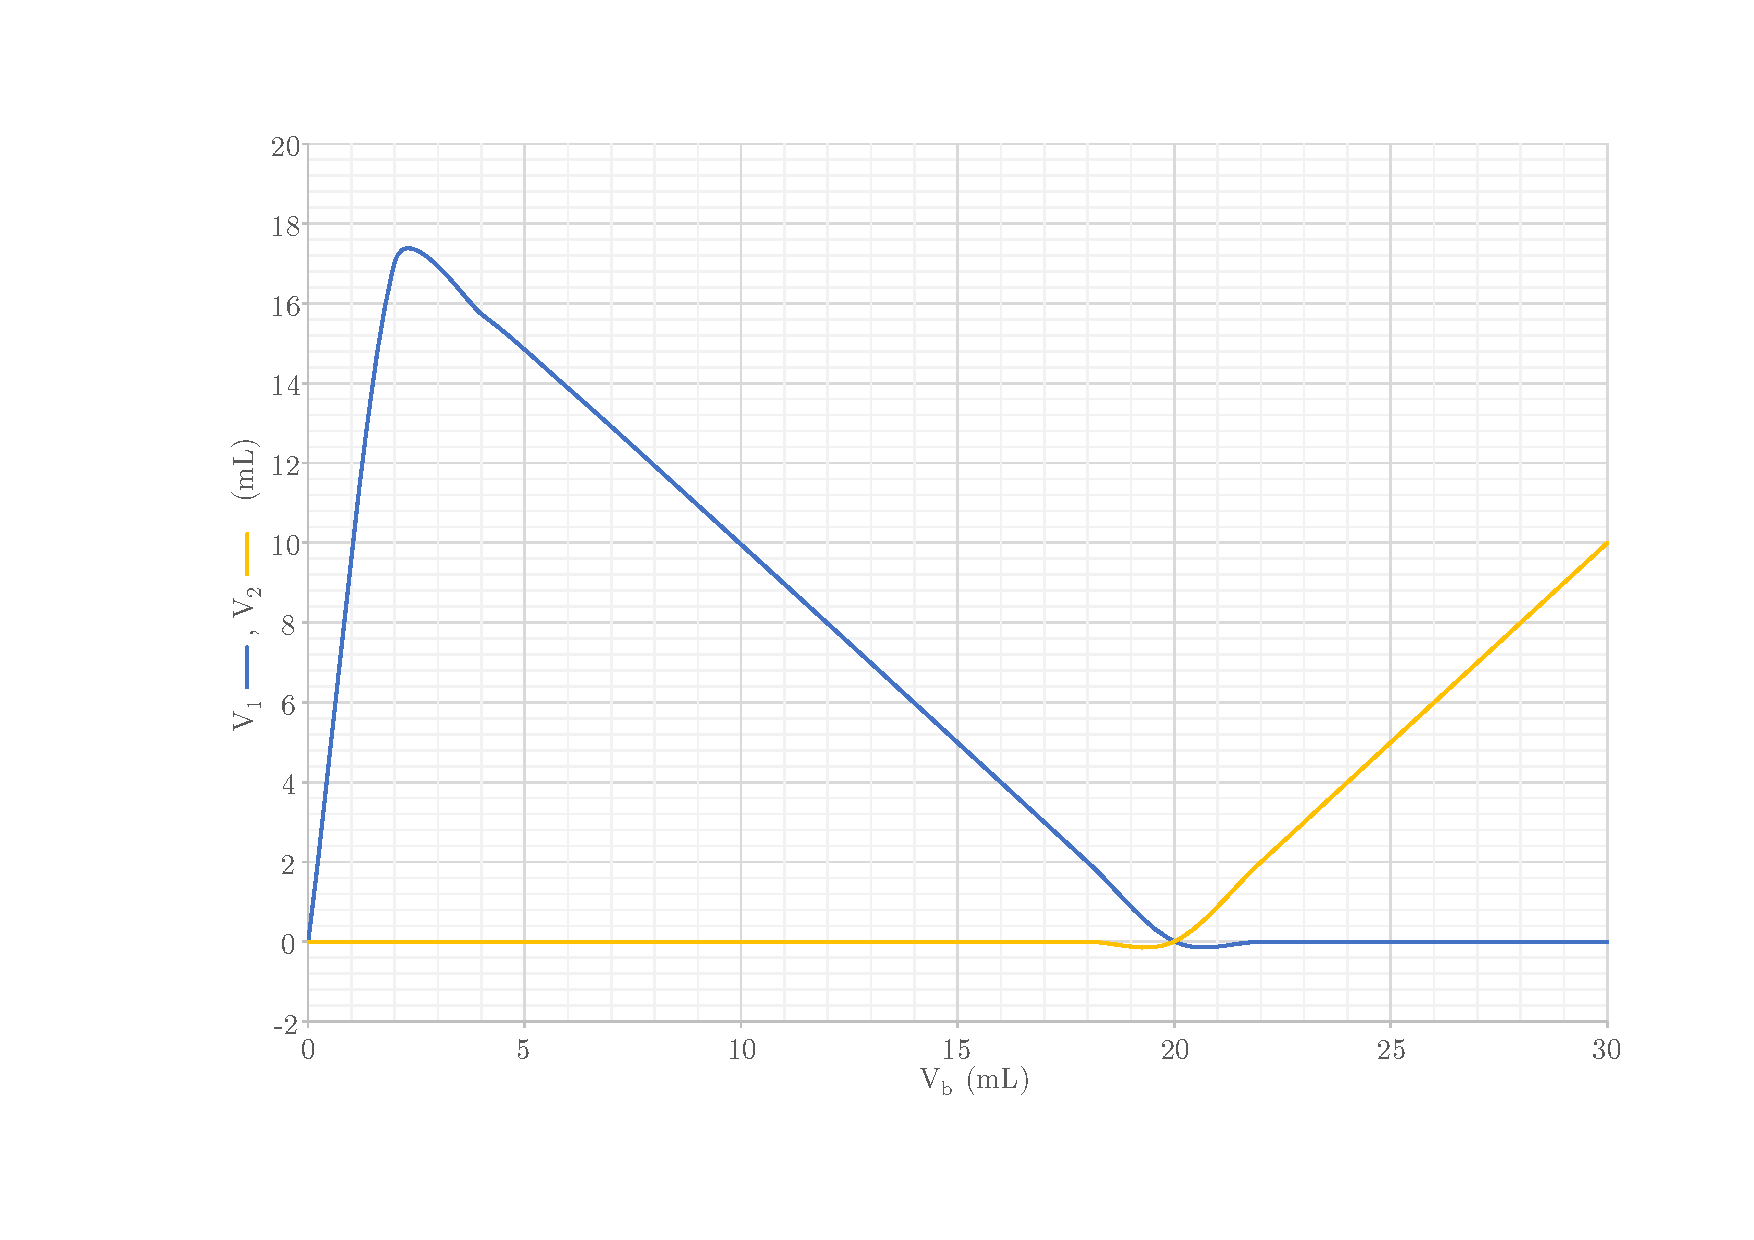
\includegraphics[width=\linewidth]{chimie/pH/gran.pdf}
        \caption{Graphe de Gran du dosage d'un acide faible par une base forte.}
    \end{figure}\vspace{-1.2em}
\end{EnvUplevel}

\question Commenter la zone $v_b\in [0 ; 2]$ mL.

\question Quels sont les avantages de la méthode de Gran par rapport à celles de la \ref{qu:eqi}.

\end{questions}
\end{exercise}

\begin{solution}
\begin{questions}
    \questioncours
    \begin{center}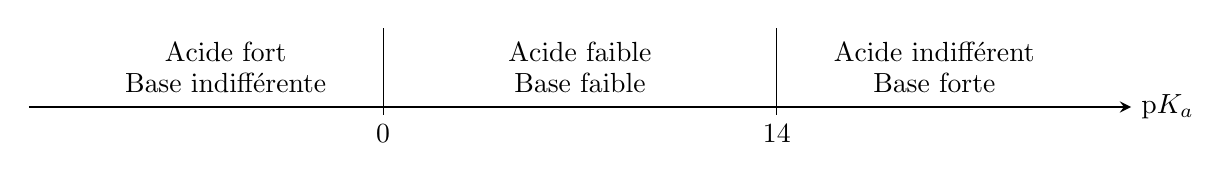
\begin{tikzpicture}[baseline=1em]
        \draw[->, >=stealth, thick] (-7,0)--(7,0) node[right]{p$K_\text{a}$};
        \draw[black] (-2.5,1)--(-2.5,-0.1) node[below]{0} ;
        \draw[black] (2.5,1)--(2.5,-0.1) node[below]{14} ;
        \node at (-4.5,.3) {Base indifférente};
        \node at (0,.3) {Base faible};
        \node at (4.5,.3) {Base forte};
        \node at (-4.5,.7) {Acide fort};
        \node at (0,.7) {Acide faible};
        \node at (4.5,.7) {Acide indifférent};
    \end{tikzpicture}\end{center}
    
    
    
    \question L'équivalence est le volume pour lequel on a introduit autant de quantité de titrant $n_\text{b}$ que de titré $n_\text{a}$
    $$n_\text{eq} = n_\text{a} = n_\text{b} \qquad \Longleftrightarrow \qquad c_\text{a} v_\text{a} = c_\text{b} v_\text{eq}.$$
    
    L'équivalence s'accompagne d'un saut de pH que l'on peut repérer par suivi pH-métrique ou grâce à un indicateur coloré, les limites de ces méthodes étant que la mesure de $v_\text{eq}$ est imprécise du fait de la largeur en volume du saut de pH qui peut être grande.
    
    \question La réaction est $\mathrm{AH + HO^- \leftrightharpoons A^- + H_2O}$. Elle a pour constante $10^{\text{p}K_\text{e} - \text{p}K_\text{a}} \gg 1$, d'où le fait qu'on puisse considérer qu'elle est totale.
    
    \question ~ \\[-2.5em]
    \begin{center}\begin{tabularx}{12cm}{r|C|C|C|C}
&
\multicolumn{1}{|c!{\makebox[0pt]{+}}}{AH}
&
\multicolumn{1}{c!{\makebox[0pt]{$\leftrightharpoons$}}}{OH$^-$}
&
\multicolumn{1}{c!{\makebox[0pt]{+}}}{A$^-$}
&
H$_2$O
\\
\hline\hline
Init. & $c_\text{a} v_\text{a}$ & $c_\text{b} v_\text{b}$ & $\varepsilon$ & $\infty$ \\
Fin. & $c_\text{a} v_\text{a} - c_\text{b} v_\text{b}$ & $\varepsilon$ & $c_\text{b} v_\text{b}$ & $\infty$ \\
& $ = c_\text{b}(v_\text{eq} - v_\text{b})$ & & & \end{tabularx}\end{center}
    
    \question Dans l'hypothèse où on se trouve dans le domaine d'Henderson, on a
    $$\text{pH} = \text{p}K_\text{a} + \log\mathrm{\dfrac{[A^-]}{[AH]}} = \text{p}K_\text{a} + \log\dfrac{\frac{c_\text{b}v_\text{b}}{v_\text{tot}}}{\frac{c_\text{b}(v_\text{eq} - v_\text{b})}{v_\text{tot}}},$$
    $$\text{d'où} \qquad v_\text{b} 10^{\text{p}K_a-\text{pH}} = v_\text{eq} - v_\text{b}.$$
       
    \question ~ \\[-2.5em]
    \begin{center}\begin{tabularx}{12cm}{r|C|C|C|C}
&
\multicolumn{1}{|c!{\makebox[0pt]{+}}}{AH}
&
\multicolumn{1}{c!{\makebox[0pt]{$\leftrightharpoons$}}}{OH$^-$}
&
\multicolumn{1}{c!{\makebox[0pt]{+}}}{A$^-$}
&
H$_2$O
\\
\hline\hline
Init. & $c_\text{a} v_\text{a}$ & $c_\text{b} v_\text{b}$ & $\varepsilon$ & $\infty$ \\
Fin. & $\varepsilon$ & $c_\text{b} v_\text{b} - c_\text{a} v_\text{a}$ & $c_\text{a} v_\text{a}$ & $\infty$ \\
 & & $ = c_\text{b}(v_\text{b} - v_\text{eq})$ & & \end{tabularx}\end{center}

    Cette fois-ci, c'est OH$^-$ qui impose sont pH. Ainsi,
    $$\text{pH} = \text{p}K_\text{e} + \log\dfrac{c_\text{b}(v_\text{b} - v_\text{eq})}{v_\text{a} + v_\text{b}}$$
    et donc en prenant en compte que pH$_\text{b} = \text{p}K_\text{e} + \log c_b$, on obtient
    $$(v_\text{b} + v_\text{a}) 10^{\text{pH}_{\,}-\text{pH}_\text{b}} = v_\text{b} - v_\text{eq}$$
    
    \question On retrouve bien les comportements de droite pour $V_1$ et $V_2$ au niveau de l'équivalence.
    
    Ici on déduit que $c_\text{a} = 2 \times 10^{-2}$ M.
    
    \question Initialement, l'hypothèse $\mathrm{[AH]}$ négligeable à l'équilibre n'est pas vérifiée car $c_\text{b} v_\text{b}$ est très petit et la réaction de dissociation de l'acide est donc prépondérante. La base réagit donc avec le H$_3$O$^+$ formé par AH.
    
    \question La méthode de Gran a pour avantage de repérer plus précisément l'équivalence mais elle repose sur des hypothèses fortes sur les composés titrés.
\end{questions}
\end{solution}
% Niveau :      PCSI *
% Discipline :  Chimie Orga I
% Mots clés :   Spectrométrie UV-visible, Réactions acidobasiques

\begin{exercise}{Influence du pH sur l'hémoglobine}{2}{PCSI}
{Chimie générale,Réactions acidobasiques,Réactions de complexation}{bermu}

L'hémoglobine est une protéine globulaire qui permet de transporter le dioxygène $\mathrm{O_2}$ dans le sang des poumons vers les autres organes. Elle est constituée de 4 complexes du fer, appelés hèmes et notés $\mathrm{HmNH_2}$ qui se lient aux molécules de $\mathrm{O_2}$ dissoutes dans le sang.

Nous nous intéressons dans cet exercice à l'influence du pH sur la ligation du $\mathrm{O_2}$ sur les hèmes.

\begin{questions}
\questioncours Théorie de Brönsted des acides et des bases. On précisera la définition du pK$_a$ et du pK$_e$.

\begin{EnvUplevel}
    Le mécanisme de ligation de l'hème avec le O$_2$ est le suivant :
    \begin{center}\schemestart[][-6]
        \chemfig{HmNH_2}
        \arrow{<=>[O$_{2\text{ (aq)}}$][$K_d$]}[0,1.5]
        \chemfig{O_2-HmNH_2}
        \arrow{<=>[H$^+_\text{ (aq)}$][?]}[-90,1.5]
        \chemfig{O_2-HmNH_3^+}
        \arrow{<=>[O$_{2\text{ (aq)}}$][$\gamma K_d$]}[-180,1.5]
        \chemfig{HmNH_3^+}
        \arrow{<=>[\rotatebox{180}{$K_a$}][\rotatebox{180}{H$^+_\text{ (aq)}$}]}[90,1.5]
    \schemestop\chemnameinit{}
    \end{center}
    
    $K_a = 2,6 \times 10^{-8}$ étant la constante d'acidité du groupe amine de l'hème, \\
    $K_d = 4,9 \times 10^{-6}$ la constante de dissociation de l'hème et du O$_2$, \\
    $\gamma = 0,73$ un facteur sans dimension.
\end{EnvUplevel}

\question Quel est le p$K_a$ de l'hème ? Sa valeur est-elle cohérente avec celle d'autres amines ? Expliciter la relation entre $K_a$, le pH et les concentrations des espèces en solutions.

\question Par analogie entre H$^+$ et O$_2$, donner la relation entre le $K_d$ et les concentrations des espèces.

\question Expliciter la constante de la réaction entre \chemfig{O_2-HmNH_2} et \chemfig{O_2-HmNH_3^+}. Quelle est la signification de $\gamma$ ?

\uplevel{On s'intéresse à la constante effective de dissociation $K_\text{eff}$ de l'hème qui prend en compte les formes acides et basiques de l'hème
$$K_\text{eff} = \mathrm{[O_2]} \times \dfrac{\Sigma \text{ espèces non liées}}{\Sigma \text{ espèces liées}}$$}

\question Expliciter l'expression de $K_\text{eff}$ en fonction des concentrations des espèces en solution puis en fonction uniquement du pH, $K_a$, $K_d$ et $\gamma$.

\uplevel{On appelle saturation S$_{\text{O}_2}$ la proportion de hèmes liés au dioxygène.}

\question Quel est le sens biologique de S$_{\text{O}_2}$ ?

\question Sachant que la pression partielle $P_{\text{O}_2}$ est proportionnelle à la concentration en $[\text{O}_2]$, montrer que S$_{\text{O}_2}$ peut s'écrire
$$\text{S}_{\text{O}_2} = \dfrac{P_{\text{O}_2}/P_{50}}{1 + P_{\text{O}_2}/P_{50}},$$
et expliciter l'expression et la signification de $P_{50}$.

\question Quel serait l'effet du CO$_2$ sur la S$_{\text{O}_2}$.

\end{questions}

\plusloin
Dash, R.K. \emph{et al, Ann Biomed Eng} \textbf{32}, 1676--1693 (2004).

\end{exercise}

\begin{solution}
\begin{questions}
    \questioncours
    \begin{itemize}
        \item Un acide de Brönsted est un donneur de H$^+$, une base de Brönsted est un accepteur de H$^+$ ;
        \item Le $K_a$ est la constante d'équilibre de la réaction
        \begin{center}\schemestart
        AH
        \arrow{<=>}[,1]
        A$^-$
        \+
        H$^+$
        \schemestop\chemnameinit{},\end{center}
        dont on déduit la relation de Henderson--Hasselbalch
        $$K_a = \mathrm{\dfrac{[A^-][H^+]}{[AH]}} \quad \Longleftrightarrow \quad \text{p}K_a = -\log K_a = \text{pH} - \log\mathrm{\dfrac{[A^-]}{[AH]}}.$$
        \item Le $K_e = 10^{-14}$ à 25$^\circ$C est la constante d'équilibre de la réaction d'autoprotolyse de l'eau
        \begin{center}\schemestart
        H$_2$O
        \arrow{<=>}[,1]
        H$^+$
        \+
        HO$^-$
        \schemestop\chemnameinit{},\end{center}
        dont on déduit la relation du produit ionique de l'eau
        $$K_e = \mathrm{[H^+][OH^-]}.$$
    \end{itemize}
    
    \question $\text{p}K_a = -\log K_a = 5,6$, ce qui est beaucoup plus bas que les amines ($\sim$ 9). La relation d'Henderson--Hasselbalch donne :
    \hfill $K_a = \mathrm{\dfrac{[HmNH_2][H^+]}{[HmNH_3^+]}}.$ \hfill ~
    
    \question Par analogie : \hfill $K_d = \mathrm{\dfrac{[HmNH_2][O_2]}{[O_2\cdot HmNH_2]}}.$ \hfill ~
    
    \question La constante de la réaction $\mathrm{HmNH_2 \longrightarrow O_2\cdot HmNH_3^+}$ étant $\gamma K_a K_d$, la constante de la réaction $\mathrm{HmNH_3^+ \longrightarrow O_2\cdot HmNH_3^+}$ est $\gamma K_a K_d$ est $\gamma K_a$.
    
    \question $K_\text{eff} = \mathrm{[O_2] \times \dfrac{[HmNH_2] + [HmNH_3^+]}{[O_2\cdot HmNH_2] + [O_2\cdot HmNH_3^+]}}
    = K_d \times \mathrm{\dfrac{[O_2\cdot HmNH_2] + \gamma [O_2\cdot HmNH_3^+]}{[O_2\cdot HmNH_2] + [O_2\cdot HmNH_3^+]}}$
    $$\text{d'où} \qquad K_\text{eff} = K_d \dfrac{1 + \dfrac{[H^+]}{K_a}}{1 + \dfrac{1}{\gamma}\,\dfrac{[H^+]}{K_a}}$$
    
    \question La S$_{\text{O}_2}$ représente la fraction d'hémoglobine qui transporte effectivement du O$_2$. C'est le marqueur biologique de l'efficacité de la respiration.
    
    \question Si $P_{\text{O}_2} = \kappa_\textsc{h} \mathrm{[O_2]}$, avec $\kappa_\textsc{h}$ appelé la constante de Henry du O$_2$, alors :
    $$\mathrm{S_{O_2}} = \dfrac{\mathrm{[O_2]}/K_\text{eff}}{1 + \mathrm{[O_2]}/K_\text{eff}} = \dfrac{P_{\text{O}_2}/P_{50}}{1 + P_{\text{O}_2}/P_{50}},$$
    avec $P_{50} = \kappa_\textsc{h}K_\text{eff}$, la pression partielle en O$_2$ nécessaire à avoir une S$_{\text{O}_2}$ à 50\%.
    
    \question L'hème peut également complexer le CO$_2$ et va donc faire diminuer la S$_{\text{O}_2}$.
    
\end{questions}
\end{solution}

\section{Réactions de précipitation}
\begin{exercise}{Solubilité de l'arséniate de cuivre}{1}{PCSI}
{solubilite,Equilibres chimiques}{lelay}

L'arséniate de cuivre (II) Cu$_3$(AsO$_4$)$_2$ lorsqu'il est plongé dans l'eau libère des ions cuivre (II) Cu$^{2+}$ et des ions arséniates AsO$_4^{3-}$. Sa solubilité dans l'eau pure à 25$^o$C est de 1.74~g.L$^{-1}$. 

\begin{questions}

    \question En déduire sa solubilité molaire et son $pK_s$.
    
    \uplevel{On mélange un volume $V_1 = 10$~mL de solution de sulfate de cuivre (II) à $c_1 = 1.6\cdot10^{-2}$~mol.L$^{-1}$ et un volume $V_2 = 40$~mL de solution d'arséniate de sodium à $c_2 = 2.0\cdot10^{-2}$~mol.L$^{-1}$.}

    \question Observe-t-on l'apparition d'un précipité ?

    \question Même question avec $c_1 = 8.0\cdot 10^{-2}$~mol.L$^{-1}$.
    
\end{questions}
Données : $M(\text{Cu}) = 63.5$~g.mol$^{-1}$, $M(\text{As}) = 75$~g.mol$^{-1}$ et $M(\text{O}) = 16$~g.mol$^{-1}$
\end{exercise}

\begin{solution}
\begin{questions}

    \question Masse molaire totale 468.5 g/mol d'où solubilité molaire 3.71~mmol/L
    
    $n$ moles dans un litre d'eau pure donnent $3s$ moles de Cu$^{2+}$ et $2s$ moles de AsO$_4^{3-}$ d'où $K_s = (3s)^3(2s)^2  =108 s^5$ avec $s = 3.71$~mmol/L d'où $K_s = 7.59\cdot 10^{-11}$ et $pK_s = -\log K_s = 10.1$
    
    \question Concentration en cuivre : $3.2$~mmol/L ; en ions arséniates $16$~mmol/L ; quotient réactionnel $Q = 8.4\time 10^{-12}$.
    
    $Q < K_s$ \textbf{donc il n'y a pas précipitation}
    
    \question Concentration en cuivre : $16$~mmol/L ; quotient réactionnel $Q = 1.0\time 10^{-9}$.
    
    $Q > K_s$ \textbf{donc il y a précipitation}
    
\end{questions}
\end{solution}

\begin{exercise}{Effet d'ion commun}{1}{PCSI}
{solubilite,Equilibres chimiques}{lelay}

Le chlorure d'argent est un solide dont la solubilité dans l'eau pure est de 1.92~mg/L.

\begin{questions}

    \question En déduire sa solubilité molaire et son $pK_s$.
    
    \uplevel{On verse maintenant du chlorure d'argent non pas dans l'eau pure mais dans une solution de chlorure de potassium de concentration $c$.}

    \question Sans calculs, que dire de la solubilité du chlorure d'argent dans ce cas ?

    \question Trouve la solubilité du chlorure d'argent pour $c = 10$~mmol/L.
    
\end{questions}
Données : $M(\text{Ag}) = 107.87$~g.mol$^{-1}$, $M(\text{Cl}) = 35.45$~g.mol$^{-1}$
\end{exercise}

\begin{solution}
\begin{questions}

    \question Masse molaire totale 143.32 g/mol d'où solubilité molaire $1.341\times 10^{-5}$~mol/L
    
    $n$ moles dans un litre d'eau pure donnent $s$ moles de Ag$^{+}$ et $s$ moles de Cl${-}$ d'où $K_s = s^2$ avec $s = 1.341\times 10^{-5}$~mol/L d'où $pK_s = -\log K_s = 9.752$
    
    \question Il y a déjà du chlore ionique dans la solution, la solubilité sera donc moindre.
    
    \question On a cette fois $Ks = s (c + s)$. Si on est malin on voit que nécessairement $s \ll c$, sinon il faut résoudre une équation du second degré. À la fin, $s = 1.8\times 10^{-8}$ mol/L
    
\end{questions}
\end{solution}

\begin{exercise}{Mélange d'halogénure d'argent}{1}{PCSI}
{solubilite,Equilibres chimiques}{lelay}

On dispose dans un bécher d’un volume $V_0 = 100$~mL d’une solution aqueuse de chlorure de sodium $C_1 = 100$~mmol/L et de bromure de sodium $C_2 = 200$~mmol/L. Les deux composés sont supposés parfaitement dissous. On dispose d’autre part d’une solution de nitrate d’argent de concentration $C = 1.00$~mol/L dans une burette de 50 mL.

\begin{questions}

    \question Tracer les domaines d'existence des précipités AgCl et AgBr en fonction de $p\text{Ag}$ ($p\text{Ag}=10^{-[Ag^+]/C^0}$)
    
    \uplevel{On introduit maintenant progressivement le nitrate d'argent de la burette dans le becher.}

    \question Sans calculs, que va-t-il se passer ? Peut-on récupérer un précipité absolument pur ? Lequel ?

    \question Quel est la quantité maximale théorique de ce précipité pur qu'il est possible de récupérer ? Calculer le rendement de cette opération.
    
\end{questions}
Données : $pK_s(\text{AgCl}) = 9.8$, $pK_s(\text{AgBr}) = 12.3$.
\end{exercise}

\begin{solution}
\begin{questions}

    \question Masse molaire totale 143.32 g/mol d'où solubilité molaire $1.341\times 10^{-5}$~mol/L
    
    $n$ moles dans un litre d'eau pure donnent $s$ moles de Ag$^{+}$ et $s$ moles de Cl${-}$ d'où $K_s = s^2$ avec $s = 1.341\times 10^{-5}$~mol/L d'où $pK_s = -\log K_s = 9.752$
    
    \question Quand $p\text{Ag}$ diminue, càd quand $[\text{Ag}^+]$ augmente, AgBr se forme, puis AgCl à partir du moment où $p\text{Ag}$ passe en dessous de 8.8. On peut donc obtenir AgBr pur.
    
    \question Le cas limite correspond à arrêter de verser lorsque $p\text{Ag} = 8.8$ i.e. $[Ag^+] = 10^{-8.8}$ M. 

    On a alors $[Br^-] = \frac{K_s}{[Ag^+]} = 10^{-3.5}$ M.

    Soit $V$ le volume versé et $n$ la quantité de solide formée. Alors on a 
    \begin{align*}
        C_2 V_0 &= [Br](V_0 + V) + n \\
        C V &= [Ag](V_0 + V) + n \\
    \end{align*}
    On en déduit $V(C+[Br]-[Ag]) = V_0(C_2 + [Ag]-[Br])$. Puisque $[Ag], [Br] \ll C_2, C$ alors $V\approx V_0 C_2/C = 20$~mL.
    D'où $n = C_2 V_0 - [Br] (V_0+V) = 0.200*0.1 - 10^{-3.5} (0.1 + 0.02) = 19.96$ mmol. Au début on en avait 20.0, d'où un rendement de 99.8 \%.
\end{questions}
\end{solution}
\begin{exercise}{Compétition ente précipités}{2}{PCSI}{Chimie générale, Réactions de précipitation, Solubilité}{chocron}

On étudie la compétition entre deux précipités : en présence d'ions iodure, les ions Pb$^{2+}$ donnent un précipité jaune et les ions Hg$^{2+}$ un précipité rouge-orangé. 

\begin{questions}
\questioncours  Critère de précipitation d'un solide en solution aqueuse.

\begin{EnvUplevel}
Lorsqu'on ajoute goutte à goutte une solution contenant des ions Hg$^{2+}$ dans un tube à essais contenant un précipité d'iodure de plomb, le précipité devient rouge-orangé dès les premières gouttes.
\end{EnvUplevel}

\question Que peut-on conclure de cette observation? \'Ecrire l'équation de la réaction (R) qui modélise le phénomène.

\begin{EnvUplevel}
On dispose d'une solution d'ions iodure de concentration $\mathrm{[I^-]_0} = 4\times 10^{-3}$ mol$\cdot$L$^{-1}$ et de deux béchers contenant respectivement 20 mL d'une solution de Pb$^{2+}$ d'une part et Hg$^{2+}$ d'autre part, de concentration $C_0$ = 0,1 mol$\cdot$L$^{-1}$. 
Dans chaque bécher, on ajoute une goutte de la solution d'ions iodure : on observe la formation d'un précipité rouge-orangé dans un bécher mais l'autre solution reste limpide.
\end{EnvUplevel}

\question Donner l'équation de la réaction ayant lieu. Sachant que le volume d'une goutte est de l'ordre de 0,05 mL, en déduire une borne inférieure du produit de solubilité de PbI$_2$ et une borne supérieure de celui de HgI$_2$.

\begin{EnvUplevel}
Le document ci-dessous correspond à la simulation de l'ajout d'une solution d'ions iodure à une solution équimolaire en ions Pb$^{2+}$ et Hg$^{2+}$, toutes les deux à 0,1 mol$\cdot$L$^{-1}$ :

\begin{figure}[H]
    \centering
    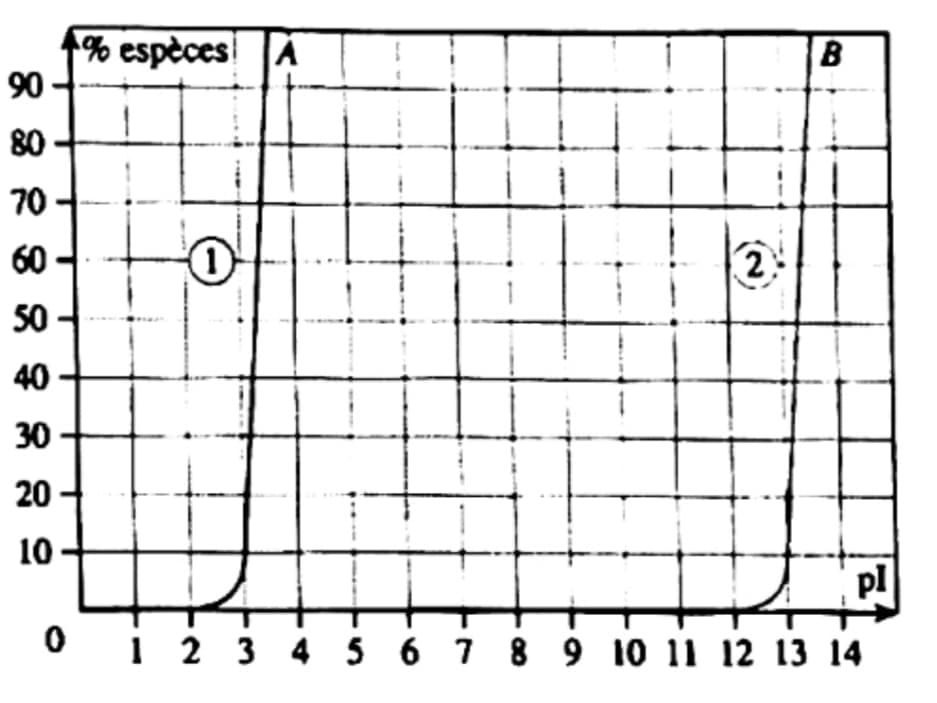
\includegraphics[width=0.8\linewidth]{chimie/precipitation/precipitationLC.jpg}
    \vspace{-1em}
    \caption[Pourcentage de cations métalliques présents dans des solutions d'ions Pb$^{2+}$ et d'ions Hg$^{2+}$  en fonction de la concentration d'ions I$^-$ ajoutés $\mathrm{pI = -\log [\text{I}^-]}$.]{Pourcentage de cations métalliques présents dans des solutions d'ions Pb$^{2+}$ et d'ions Hg$^{2+}$ en fonction de la concentration d'ions I$^-$ ajoutés $\mathrm{pI = -\log [\text{I}^-]}$.}
\end{figure}
\end{EnvUplevel}

\question Que représentent les points anguleux? Identifier les deux courbes tracées (on note que les courbes \textcircled{1} et \textcircled{2} sont strictement égales à 100\% à droite des points A et B respectivement)

\question  En déduire les produits de solubilité de PbI$_2$ et HgI$_2$. Commenter.

\question Déterminer la constante d'équilibre de la réaction (R). Commenter.

\end{questions}
\end{exercise}

\begin{solution}
\begin{questions}

\questioncours Exemple de HgI$_2$. La réaction $\mathrm{HgI_2}_\text{s} \leftrightharpoons \mathrm{Hg^{2+}_\text{aq} + 2 {I^-}_\text{aq}}$ admet pour constante d'équilibre $K_s$. Le solide n'existe que pour $Q_r > K_s$ :
    \begin{center}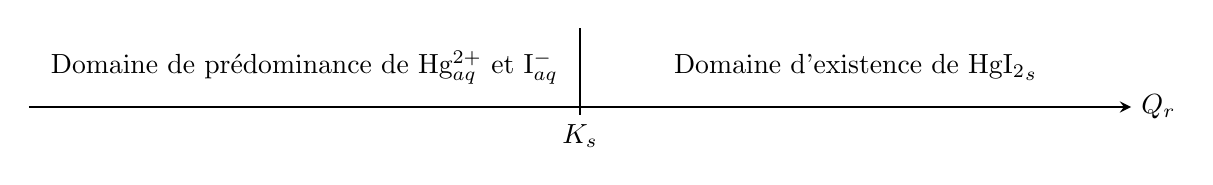
\begin{tikzpicture}[baseline=1em]
        \draw[->, >=stealth, thick] (-7,0)--(7,0) node[right]{$Q_r$};
        \draw[black] (0,1)--(0,-0.1) node[below]{$K_s$} ;
        \node at (-3.5,.5) {Domaine de prédominance de Hg$^{2+}_\text{aq}$ et I$^-_\text{aq}$};
        \node at (3.5,.5) {Domaine d'existence de $\mathrm{HgI_2}_\text{s}$};
    \end{tikzpicture}\end{center}

\question Lorsqu'on introduit des ions mercuriques dans une solution en présence de précipité d'iodure de plomb, le précipité de plomb (jaune) disparaît et le précipité de mercure (rouge-orangé) apparaît.
Il se produit donc la réaction
\begin{equation}
    \mathrm{{PbI_2}_\text{(s)} + {Hg^{2+}}_\text{(aq)} \rightleftharpoons {Pb^{2+}}_\text{(aq)} + {HgI_2}_\text{(s)}} \qqtext{de constante} K. \tag{R}
\end{equation}
    
Cette réaction est très favorable dans le sens direct ($K\gg 1$).
HgI$_2$ est donc moins soluble dans l'eau que PbI$_2$.


\question Il y a formation d'un précipité rouge-orangé donc HgI$_2$. La réaction de formation est
$$\mathrm{Hg^{2+} + 2I^- \rightarrow HgI_2}.$$

D'après le critère de précipitation en solution, le précipité se forme si $Q_r > K_{s,\mathrm{HgI_2}}$, donc $$\mathrm{[Hg^{2+}][I^-]^2}  \geqslant K_{s,\mathrm{HgI_2}}, \quad \Longleftrightarrow \quad \mathrm{[Hg^{2+}] = 0,1 \ mol\cdot L^{-1}},$$
en négligeant la variation de volume $V_g$ ajouté par la goutte.
$$\mathrm{[I^-]= [I^-]_0} \dfrac{V_g}{V_0} = \mathrm{1\cdot10^{-5} mol\cdot L^{-1}}$$

On a donc $Q_r = 10^{-11} \geqslant K_{s,\mathrm{HgI_2}},$

Avec le même calcul pour PbI$_2$, et dans ce cas, comme le précipité ne se forme pas, $Q_r \leqslant K_s$, on trouve 
10$^{-11} \leqslant K_{s,\mathrm{PbI_2}}$.

\question Initialement la solution ne contient pas de I$^-$ (pI $\rightarrow + \infty$) et les ions Pb$^{2+}$ et Hg$^{2+}$ sont tous les deux à la concentration C$_0$ = 0,100 mol$\cdot$L$^{-1}$. En pourcentage, 100\% des cations sont en solution, la solution est limpide.

Puis on ajoute des ions I$^-$, rien ne se passe jusqu'au point B (en partant de la droite i.e. en ajoutant des ions iodure) où pI$_B = 13,6$. 

Le point B est un point anguleux de la courbe \textcircled{2} ; cela traduit \textbf{une rupture d'équilibre, en l'occurrence, l'apparition d'un précipité}. D'après la question précédente, on sait que Hg$^{2+}$ est un meilleur accepteur de I$^-$ que Pb$^{2+}$ : c'est donc le précipité HgI$_2$ qui apparaît en B. Si on continue d'ajouter du I$^-$, cela entraîne la précipitation de HgI$_2$ et donc la diminution de la concentration en Hg$^{2+}$. 
\textbf{La courbe \textcircled{2} représente donc la concentration de Hg$^{2+}$, exprimée en pourcentage de C$_0$.}

Lorsque Hg$^{2+}$ a quasiment disparu, le pI diminue de nouveau puisqu'on ajoute des ions iodure en solution. 
La courbe \textcircled{1} reste à 100\% jusqu'en A, où un nouveau point anguleux survient (pI$_A$=3,6) qui traduit l'apparition du second précipité PbI$_2$. 
\textbf{La courbe \textcircled{1} représente donc la concentration de Pb$^{2+}$, exprimée en pourcentage de C$_0$.}

\question Pour trouver les produits de solubilité, on utilise les coordonnées des points anguleux.

Par exemple, pour HgI$_2$, en B, le premier grain de précipité apparaît et donc on peut utiliser le $K_s$. Par ailleurs, la proportion de Hg$^{2+}$ est encore de 100\% donc sa concentration vaut 0,100 mol$\cdot$L$^{-1}$.
On a donc
$$K_{s,\mathrm{HgI_2}} = \mathrm{[Hg^{2+}]_B \times [I^-]_B^2} = C_0 \times 10^{-2pI_B} = 6 \cdot 10^{-29}.$$  

De même,
$$K_{s,\mathrm{PbI_2}} = \mathrm{[Pb^{2+}]_A \times [I^-]_A^2} = C_0 \times 10^{-2pI_A} = 6 \cdot 10^{-9}.$$   

Ces résultats sont en accord avec les bornes inférieure et supérieure déterminées à la question 3.

\question $K = \dfrac{K_{s,\mathrm{PbI_2}}}{K_{s,\mathrm{HgI_2}}} = 10^{+20} \gg 1$ comme prévu.

\end{questions}
\end{solution}
% Niveau :      PCSI *
% Discipline :  Chimie Orga I
% Mots clés :   Spectrométrie UV-visible, Réactions acidobasiques

\begin{exercise}{Méthode de Mohr}{2}{PCSI}
{Chimie générale,Réactions de précipitation,Mohr (méthode de),Titrage}{bermu}

Dans cet exercice, on étudie une solution de chlorure de sodium de concentration inconnue $c_0 \sim 10^{-2}$ M à l'aide d'une solution de nitrate d'argent.

\begin{questions}
\questioncours Critère de précipitation d'un solide en solution aqueuse. \\ On prendra l'exemple du chlorure d'argent.

\question Quelle est la solubilité $s_1$ du chlorure d'argent ?

\begin{EnvUplevel}
    On introduit dans un becher un volume $v_0 = 40,0$ mL de la solution que l'on souhaite titrer. Cette solution est titrée par une solution de nitrate d’argent de concentration $c_1 = 0,0250$ M.
    
    On considérera pour simplifier que la dilution est négligeable.
\end{EnvUplevel}

\question \'Ecrire la réaction support de titrage.

\question Sachant qu'une goutte délivrée par une burette a environ un volume $v_g \simeq 0,05$ mL, la réaction de titrage débute-t-elle dès la première goutte de nitrate d’argent versée ?

\question Définir l'équivalence et donner l'expression du volume équivalent $V_\text{eq}$ en fonction des données de l'exercice.

\begin{EnvUplevel}
    Afin de détecter expérimentalement cette équivalence, on ajoute dans la solution avant le titrage quelques gouttes d'une solution incolore de chromate de sodium Na$_2$CrO$_4$.
\end{EnvUplevel}

\question Sachant que les ions chromate sont susceptibles de donner avec les ions argent (I) un précipité rouge vif de chromate d’argent, calculer la concentration $c_2$ en ions chromate à apporter dans la solution initiale pour que l’apparition du précipité rouge se produise exactement à l’équivalence et permette ainsi de détecter celle-ci avec précision.

\question En quoi la précision du titrage serait-elle affectée si on introduisait au début du titrage une concentration 10 fois plus importante de chromate de sodium ? 10 fois moins ? Commenter.

\question On trouve suite à l'expérience $v_\text{eq} = 24$ mL. Quelle est la valeur de $c_0$ ? \\
Estimer l'incertitude sur cette valeur.

\end{questions}

\paragraph{Données : }~\\
AgC$\ell$ \quad p$K_{s1} = 9,8$, \\
Ag$_2$CrO$_4$ \quad p$K_{s2} = 12,0$.


\end{exercise}

\newpage

\begin{solution}
\begin{questions}
    \questioncours La réaction $\mathrm{AgC\ell_\text{s} \leftrightharpoons {Ag^+}_\text{aq} + {C\ell^-}_\text{aq}}$ admet pour constante d'équilibre $K_{s1}$. Le solide n'existe que pour $Q_{r1} > K_{s1}$ :
    \begin{center}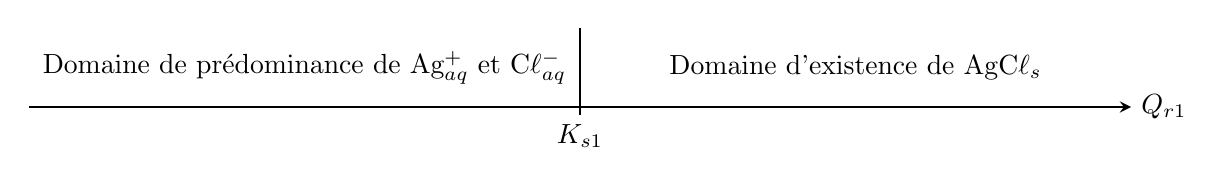
\begin{tikzpicture}[baseline=1em]
        \draw[->, >=stealth, thick] (-7,0)--(7,0) node[right]{$Q_{r1}$};
        \draw[black] (0,1)--(0,-0.1) node[below]{$K_{s1}$} ;
        \node at (-3.5,.5) {Domaine de prédominance de Ag$^+_\text{aq}$ et C$\ell^-_\text{aq}$};
        \node at (3.5,.5) {Domaine d'existence de AgC$\ell_\text{s}$};
    \end{tikzpicture}\end{center}
    
    \question On suppose qu'on introduit une quantité grande de AgC$\ell$ dans de l'eau pure. \`A l'équilibre
    $$K_{s1} = \mathrm{[Ag^+][C\ell^-]} = s^2,$$
    donc $s = 10^{-\text{p}K_{s1}/2} = 1,3 \times 10^{-5}$ M.
    
    \question La réaction est
    $$\mathrm{{Ag^+}_\text{aq} + {C\ell^-}_\text{aq} \longrightarrow AgC\ell_\text{s}}$$
    
    \question Au début, [Ag$^+$] $= 0$.
    \`A la première goutte, [Ag$^+$]$ = \dfrac{c_1 v_g}{v_0}$ donc
    $$Q_{r1} = c_0 c_1 \dfrac{v_g}{v_0} > K_{s1} \qqtext{ou} c_0 > \dfrac{K_{s1} v_0}{c_1 v_g} \simeq 5,1 \times 10^{-6} \text{ M},$$
    le précipité apparaît donc dès la première goutte de titrant versée si la concentration $c_0$ est supérieure à $5,1 \times 10^{-6}$ M.
    
    \question Par définition, l’équivalence est obtenue lorsqu’on a apporté Ag$^+$ et C$\ell^-$ dans les proportions st{\oe}chiométriques de la réaction de titrage, ici 1:1, soit
    $$n_\text{eq} = n_\mathrm{C\ell^-} = n_\mathrm{Ag^+} \qquad \Longleftrightarrow \qquad c_0 v_0 = c_1 v_\text{eq}.$$
    
    \question \`A l’équivalence le titrant a consommé exactement le titré : la réaction est quasi-totale. Il ne reste donc qu'une trace d'ions Ag$^+$ et C$\ell^-$, égale à la solubilité $s$ calculée à la question 2.
    
    Si on veut que la solution devienne saturée en Ag$_2$CrO$_4$ à l'équivalence, il faut que la concentration en CrO$_4^{2-}$, $c_2$ soit telle que 
    $$Q_{r2} = \mathrm{[Ag^+]^2 [CrO_4^{2-}]} = s^2 c_2 > K_{s2} \qqtext{ou} c_2 = \dfrac{K_{s2}}{K_{s1}} = 6,3 \times 10^{-3} \text{ M}.$$
    
    \question Si on apporte $\gamma$ (10 ou 1/10) plus de fois d’ions chromate, $\mathrm{[CrO_4^{2-}]} = \gamma c_2$, le précipité Ag$_2$CrO$_4$ va apparaître (avant l'équivalence si $\gamma > 1$ et après si $\gamma < 1$) lorsque
    $$\mathrm{[Ag^+]}_\text{seuil} = \sqrt{\dfrac{K_{s2}}{\gamma c_2}} = \sqrt{\dfrac{K_{s1}}{\gamma}},$$
    et donc quand
    $$\mathrm{[Cl^-]}_\text{seuil} = \dfrac{K_s}{\mathrm{[Ag^+]}} = \dfrac{s}{\sqrt{\gamma}},$$
    ce qui génère une erreur sur le volume équivalent de l'ordre de
    $$\dfrac{\mathrm{[Cl^-]}_\text{seuil} - c_0}{c_0} = (\gamma^{-1/2} - 1)s/c_0$$
    Ainsi l'erreur est très faible et la concentration $c_2$ a peu d'influence sur le résultat.
    
    \question On trouve
    $$c_0 = \dfrac{c_1 v_\text{eq}}{v_0} = 0,015 \text{ M}.$$

\end{questions}
\end{solution}
% Niveau :      PCSI *
% Discipline :  Chimie Orga I
% Mots clés :   Spectrométrie UV-visible, Réactions acidobasiques

\begin{exercise}{Précipitation sélective}{2}{PCSI}
{Chimie générale,Réactions de précipitation, Solubilité, Précipitation sélective}{bermu}

Actuellement, les métaux présents dans les effluents liquides industriels sont précipités sous forme de boues d'hydroxydes métalliques qui sont stockées comme déchets ultimes sans possibilité de valorisation. Nous allons étudier une alternative écologique consistant à les précipiter sélectivement pour les séparer et les revaloriser.

\begin{questions}
\questioncours Paramètres influençant la solubilité des sels en solution aqueuse. \\
On donnera les tendances générales et on illustrera d'exemples.

\begin{EnvUplevel}
    On considère tout d'abord le cas de l'aluminium. L'hydroyde d'aluminium $\mathrm{{Al{(OH)}_3}_{(s)}}$ est un solide formé par les équilibres successifs suivants :
    $$\mathrm{{Al^{3+}}_{(aq)} + 4 {OH^-}_{(aq)} \overset{\mathnormal{K_s} = 10^{-32}}{\leftrightharpoons} {Al{(OH)}_3}_{(s)} + {OH^-}_{(aq)}  \overset{\mathnormal{K_f} = 10^2}{\leftrightharpoons} {[Al{(OH)}_4]^-}_{(aq)}}.$$
    
    On considérera la quantité globale en aluminium fixée à [Al]$_\text{tot} = 10^{-2}$ mol$\cdot$L$^{-1}$.
\end{EnvUplevel}

\question \'Ecrire le produit de solubilité $K_{s,\mathrm{{Al{(OH)}_3}}}$ et donner le critère de précipitation de $\mathrm{{Al{(OH)}_3}_{(s)}}$.

\question Quel est le comportement acido-basique $\mathrm{{Al{(OH)}_3}_{(s)}}$ ? \\ Calculer les pH d'apparition pH$_a$ et de disparition pH$_d$ de $\mathrm{{Al{(OH)}_3}_{(s)}}$ puis tracer le diagramme d'existence de cet hydroxyde en fonction du pH.

\question Tracer qualitativement $\log s$ en fonction du pH, $s$ étant la somme des concentrations des espèces de l'aluminium solubles. \\
On veillera bien à distinguer les différents cas vus à la question précédente.

\question Quel est le pH optimal pH$^\ast$ pour précipiter  $\mathrm{{Al{(OH)}_3}_{(s)}}$ ?

\begin{EnvUplevel}
    Le problème de la précipitation des hydroxydes est qu'elle est peu sélective et ne permet pas de traiter tous le métaux comme l'illustre la figure ci-dessous : \vspace{-.4em}
    
    \begin{figure}[H]
        \centering
        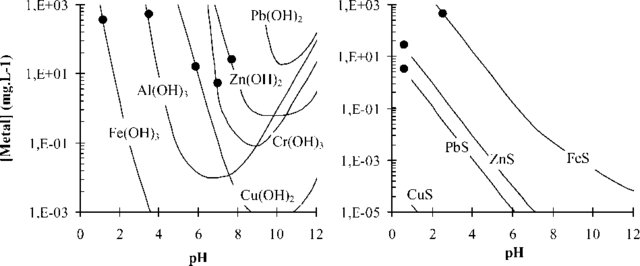
\includegraphics[width=.9\linewidth]{chimie/precipitation/precipitation_selective.png}
        \caption{Solubilités des hydroxydes métalliques et des sulfures métalliques en fonction du pH.}
    \end{figure}
\end{EnvUplevel}

\question Justifier le défaut de sélectivité de la précipitation d'hydroxydes.

\question{\sffamily Question ouverte :} établir un protocole expérimental chiffré pour traiter un mélange d'hydroxydes métalliques industriel en vous aidant de la Fig. 1 et des données ci-dessous. \\
On pourra commencer par un mélange contenant uniquement de l'aluminium et du cuivre par exemple.

\end{questions}

\paragraph{Données :} masses molaires (g$\cdot$mol$^{-1}$) \vspace{-1em}

\begin{table}[H]
    \centering
    \begin{tabularx}{0.8\linewidth}{CCCCCCCCCCCC}
        H   & O  & Na & Al & S  & Cr & Fe & Cu & Zn & Pb \\ \hline
        1,0 & 16 & 23 & 27 & 32 & 52 & 56 & 64 & 66 & 82 \\ \hline\hline
    \end{tabularx}
\end{table}

\plusloin Marina Maya Marchioretto emph{et al.} Heavy Metals
Precipitation in Sewage Sludge, \textit{Separation Science and Technology}, Vol. 40, no. 16, \textbf{2005}, 3393--3405. \vspace{-.5em}
\end{exercise}

\begin{solution}
\begin{questions}
    \questioncours
    \begin{itemize}
        \item \emph{Température :} globalement, la solubilité augmente avec la température (question d'entropie). Cela peut être utile pour dissoudre à chaud ou faire de la cristallisation.
        
        \item \emph{Effet d'ion commun :} La présence d'un ion faisant partie du sel (ion commun) déjà présent en solution augmente le quotient de réaction $Q_r$ et donc diminue la solubilité du sel.
        
        \item \emph{Compétition avec d'autres équilibres :} acide-base , complexation... Ces réactions consomment en partie un ion faisant partie du sel ce qui diminue $Q_r$ et augmente la solubilité.
        
        \end{itemize}
    
    \question À l'équilibre, $Q_r = \mathrm{[Al^{3+}][OH^-]^3} = K_s$ : il y a précipitation si $Q_r > K_s$, en deçà, c'est rupture d'équilibre.
    
    \question $\mathrm{{Al{(OH)}_3}_{(s)}}$ est un amphotère, à la fois acide et base. \\
    Pour l'apparition avec le $K_s$ d'après le critère précédent :
    $$K_s = \mathrm{[Al^{3+}][OH^-]^3} \quad \Longleftrightarrow \quad \text{pH}_a = \text{p}K_e - \dfrac{1}{3}\text{p}K_s - \dfrac{1}{3}\log\mathrm{[Al]_{tot}} = 4.$$
    
    De même pour la disparition
    $$K_f = \mathrm{\dfrac{[{Al(OH)_4}^-]}{[OH^-]}} \quad \Longleftrightarrow \quad \text{pH}_d = \text{p}K_e + \text{p}K_f + \log\mathrm{[Al]_{tot}} = 10.$$
    
    Le domaine d'existance de $\mathrm{{Al{(OH)}_3}_{(s)}}$ est donc $4 \leqslant \text{pH} \leqslant 10$.
    
    \question D'après la question précédente, pour $4 \leqslant \text{pH} \leqslant 10$, les deux équilibres sont atteints, donc
    \begin{align*}
        s(\text{pH}) &= \mathrm{[Al^{3+}] + [{Al(OH)_4}^-]} = K_s 10^{-3(\text{pH} - \text{p}K_e)} + K_f 10^{\text{pH} - \text{p}K_e}, \\
        \noalign{que l'on peut réécrire}
        s(\text{pH}) &= \mathrm{[Al]_{tot}}\qty(10^{-3(\text{pH} - \text{pH}_a)} + 10^{\text{pH} - \text{pH}_d}), \\
        \noalign{et donc, asymptotiquement pour pH - pH$_a$ $\ll$ 1}
        \log s(\text{pH}) &= \log\mathrm{[Al]_{tot}} + 3 \text{pH}_a - 3 \text{pH}, \\
        \noalign{et pour pH$_d$ - pH $\ll$ 1}
        \log s(\text{pH}) &= \log\mathrm{[Al]_{tot}} - \text{pH}_d + \text{pH}.
    \end{align*}
    
    \question Le pH optimal pH$^\ast$ est pour
    $$\dv{s}{\text{pH}} = 0 \quad\Longleftrightarrow\quad
    \text{pH}^\ast = \dfrac{1}{4}\log\qty(3 + 10^{3\text{pH}_a + \text{pH}_d}) \simeq \dfrac{3\text{pH}_a + \text{pH}_d}{4} = 5,5,$$
    (c'est l'interception des deux asymptotes).
    
    \question Les droites de solubilité de la Fig. 3.1 se croisent : les précipités se forment en même quantité pour pH $\geqslant 6$. Ainsi, si Fe et Al peuvent être précipités sélectivement, ce n'est pas le cas de Cu, Zn, Cr et Pb.
    
    \question{\sffamily Suggestion de protocole : }  il faut donc utiliser des sulfures pour traiter Cu, Zn ect.
    
    \begin{itemize}
        \item Partant d'une boue d'hydroxyde, on effectue une lixiviation (= acidifiaction) jusqu'à pH $\simeq 2$ avec de l'acide sulfurique par exemple (éviter les halogènes) ;
        \item Ensuite on rajoute de la soude jusqu'à pH $\simeq 3$ : Fe précipite. Filtrage, lavage, séchage ;
        \item Ensuite on rajoute de la soude jusqu'à pH $\simeq 5,5$ : Al précipite. Filtrage, lavage, séchage ;
    \end{itemize}
    A partir de cet instant, on ne peut plus être sélectif en ajoutant de la soude... On ajoute donc du sulfure de sodium Na$_2$S qui va faire précipier d'abord le Cu, puis le Pb, puis le Zn...
    
\end{questions}
\end{solution}


\section{Oxydoréduction}
\begin{exercise}{Titrage par le sulfate cérique}{3}{PCSI}{Chimie générale, Réactions de complexation, Oxydoréduction, Titrage}{chocron}

Dans un bécher, on introduit 20 mL du mélange à doser qui contient un mélange d'ions Fe$^{2+}$~(concentration $3,00 \times 10^{-2}$ mol$\cdot$L$^{-1}$) et d'ions Co$^{2+}$ (concentration inconnue). On ajoute 1,8 g d'orthophénanthroline (notée o-phen). 
On plonge dans la solution un couple d'électrode (électrode de platine et électrode au calomel saturé).
On effectue le titrage par une solution de sulfate cérique (Ce$^{4+}$) à une concentration de 10$^{-1}$ mol.L$^{-1}$ :
\begin{figure}[H]
    \centering
    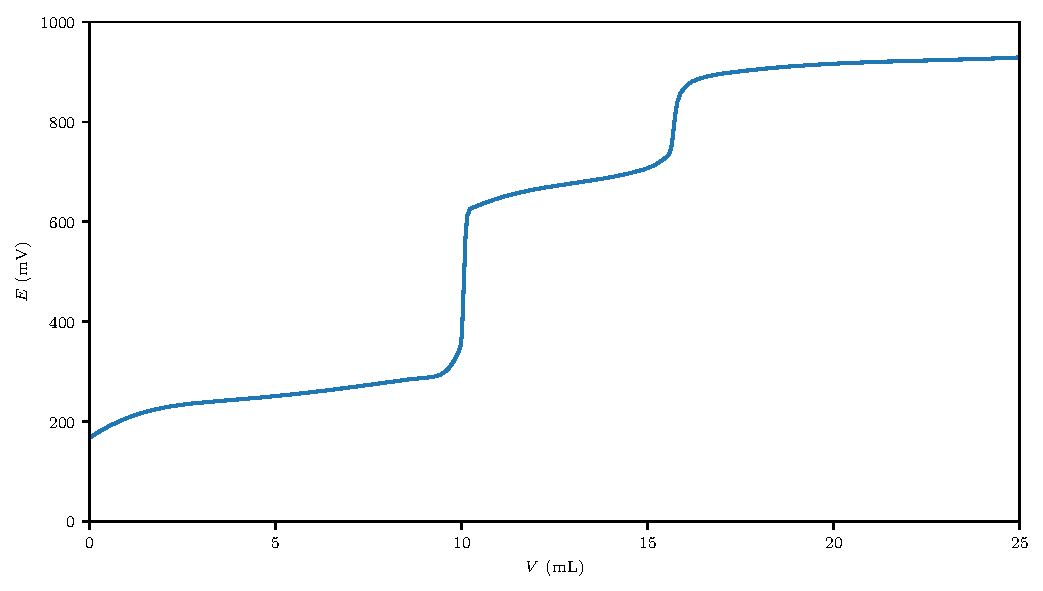
\includegraphics[width=\linewidth]{chimiePC/gene/dosage_ophen.pdf}\vspace{-1em}
    \caption{Dosage potentiométrique de la solution par le sulfate cérique.}
\end{figure}

\begin{questions}
\questioncours Quels types d'électrodes sont utilisées pour ce dosage?

\question Écrire les deux équations de dosage qui peuvent avoir lieu. Calculer leurs constantes d'équilibre. Est-ce cohérent avec la courbe de dosage observée expérimentalement?

\begin{EnvUplevel}
En réalité, les ions Fe$^{3+}$, Fe$^{2+}$, Co$^{3+}$ et Co$^{2+}$ forment avec l'orthophénanthroline des complexes très stables de formule générale [M(o-phen)$_3$]$^{n+}$.
Les ions Ce$^{4+}$ et Ce$^{3+}$ ne forment pas de complexe avec l'orthophénanthroline.  

\end{EnvUplevel}
\question Calculer la quantité de matière d'orthophénanthroline. 

\question En déduire les espèces (potentiellement) en solution avant le dosage et en déduire les réactions de dosage qui ont réellement lieu. 
\question Déterminer l'ordre des réactions de dosage.

\question En déduire la concentration en ions cobalt ainsi que les potentiels standard des deux couples impliqués dans le dosage. On supposera que tout le colbalt est complexé.

\question Que peut-on en déduire sur les constantes globales de formation des complexes considérés?
\end{questions}

\paragraph{Données : } potentiels standards $E^\circ$ dans les CNTP (en l'absence de tout agent complexant)
\begin{center}\begin{tabular}{rccc}
    \hline
    & $\mathrm{{Fe^{3+}}_{(aq)} \,/\, {Fe^{2+}}_{(aq)}}$ & $\mathrm{{Co^{2+}}_{(aq)} \,/\, {Co^{2+}}_{(aq)}}$ & $\mathrm{{Ce^{4+}}_{(aq)} \,/\, {Ce^{3+}}_{(aq)}}$ \\
    $E^\circ$ (V) & 0,77 & 1,84 & 1,44 \\ \hline\hline 
\end{tabular}\end{center}

\'Electrode au calomel saturé (ECS) : $E_\text{ref} = 244$ mV ;

On note: $e^\circ = \dfrac{RT}{\scr{F}} \ln10 = 59$ mV ; \\[-.2em]

o-phen : {\setchemfig{atom sep = 1.5 em}\chemfig{[:-30]*6(-=N-*6(-*6(-N=-=-)=-=-)=-=)}}.

\end{exercise}


\begin{solution}
\begin{questions}
\questioncours cf. cours. L'électrode de platine est une électrode du 3ème type et l'électrode de référence (au calomel saturé) est une électrode du 2ème type.

\question 
Les réactions de dosage qui peuvent avoir lieu sont :
\begin{align}
    \mathrm{Fe^{2+} + Ce^{4+}} &\longrightarrow \mathrm{Fe^{3+} + Ce^{3+}}, \tag{1} \\
    \mathrm{Co^{2+} + Ce^{4+}} &\longrightarrow \mathrm{Co^{3+} + Ce^{3+}}. \tag{2}
\end{align}

D'après la formule du cours,
\begin{align*}
    \log(K_1) &= \dfrac{E^\circ\qty\big(\mathrm{Ce^{4+} / Ce^{3+}}) - E^\circ\qty\big(\mathrm{Fe^{3+} / Fe^{2+}})}{e^\circ} = 11.2, \\
    \log(K_2) &= \dfrac{E^\circ\qty\big(\mathrm{Ce^{4+} / Ce^{3+}}) - E^\circ\qty\big(\mathrm{Co^{3+} / Co^{2+}})}{e^\circ} = -6.67.
\end{align*}
On a donc $K_1 \gg 1 \gg K_2$. La seule réaction qu'on devrait observer est donc la réaction (1). 

Or d'après la courbe de dosage, on observe deux équivalences donc deux réactions de dosage. Il se passe donc autre chose.

\question $n(\text{o-phen}) = \dfrac{1,8}{180} = 10$ mmol, alors que  $n(\mathrm{Fe^{2+}}) = 0,6$ mmol. La réaction de complexation du fer s'écrit :
$$\mathrm{Fe^{2+} + 3 \text{o-phen} \longrightarrow Fe(\text{o-phen})_3^{2+}.}$$

L'orthophénanthroline est donc en large excès par rapport au fer(II) et la réaction de complexation est quantitative. 
Il n'y a donc plus de Fe$^{2+}$ libres en solution, ils sont tous complexés.  

\question Avant le dosage sont présents en solution : le complexe Fe(o-phen)$_3^{2+}$, le complexe Co(o-phen)$_3^{2+}$ et éventuellement de l'orthophénanthroline libre (si tout le cobalt est complexé et qu'il y a un excès de ligand) ou alors du cobalt(II) libre (si tout le cobalt n'est pas complexé). 

Dans tous les cas, l'orthophénanthroline ne réagit pas avec les ions cérium(IV) et la réaction entre les ions cérium(IV) et les ions cobalt(II) libres n'a pas lieu. 

Les deux réactions de dosage correspondants aux deux équivalences observées sont donc :
\begin{align}
    \mathrm{Fe(\text{o-phen})_3^{2+} + Ce^{4+}} &\longrightarrow \mathrm{Fe(\text{o-phen})_3^{3+} + Ce^{3+}}, \tag{3} \\
    \mathrm{Co(\text{o-phen})_3^{2+} + Ce^{4+}} &\longrightarrow \mathrm{Co(\text{o-phen})_3^{3+} + Ce^{3+}}. \tag{4}
\end{align}

\question On connait la concentration en ions Fe$^{2+}$ et donc en Fe(o-phen)$_3^{2+}$ et on peut donc calculer le volume équivalent correspondant :
$$[\mathrm{Fe(\text{o-phen})_3^{2+}}] \times V_\text{tot} = [\mathrm{Ce^{4+}}] \times V_\text{eq} \quad \Longleftrightarrow \quad V_\text{eq} = 6 \text{ mL}.$$

Graphiquement on obsverse que $V_\text{eq1} = 10$ mL et $V_\text{eq2} - V_\text{eq1} = 6$ mL. 

C'est donc le dosage du cobalt complexé qui correspond à la première équivalence et la deuxième équivalence correspond au fer complexé.

\question Si on considère que tous les ions cobalt sont complexés, on a à la première équivalence :
$$[\mathrm{Co(\text{o-phen})_3^{2+}}] \times V_\text{tot} = [\mathrm{Ce^{4+}}] \times V_\text{eq1} \quad \Longleftrightarrow \quad [\mathrm{Co^{2+}}] = 5 \times 10^{-2} \mathrm{ mol\cdot L^{-1}},$$
ce qui est bien cohérent avec l'hypothèse que tous les cobalt sont complexés. 

On peut également déterminer graphiquement les $E^\circ$ des couples Fe(o-phen)$_3^{3+}$/Fe(o-phen)$_3^{2+}$ et Co(o-phen)$_3^{3+}$/Co(o-phen)$_3^{2+}$. En effet, à la demi-équivalence on a $\Delta E_{1/2\text{eq}}=E^\circ - E_\text{ref}$.

$$\text{Pour } V = \dfrac{\text{V}_\text{eq1}}{2} = 5 \text{ mL, on a } \Delta E  = E^\circ\qty\big(\text{Co(o-phen)}_3^{3+}/\text{Co(o-phen)}_3^{2+}) - E_\text{ref} \simeq 0,12 \text{ V},$$

d'où  $E^\circ(\text{Co(o-phen)}_3^{3+}/\text{Co(o-phen)}_3^{2+}$=0,36 V. 
$$\text{De même pour } V = \dfrac{\text{V}_\text{eq1}}{2} = 5 \text{ mL, on a } \Delta E  = E^\circ\qty\big(\text{Fe(o-phen)}_3^{3+}/\text{Fe(o-phen)}_3^{2+}) - E_\text{ref} \simeq 0,80 \text{ V},$$

d'où  $E^\circ(\text{Fe(o-phen)}_3^{3+}/\text{Fe(o-phen)}_3^{2+}$=1,04 V.

\question Soit M un métal (Fe ou Co), on note $\beta_{II}$ la constante de formation du complexe [M(o-phen)$_3$]$^{2+}$ et $\beta_{III}$ celle du complexe [M(o-phen)$_3$]$^{3+}$.

On montre que E$^\circ$(M(o-phen)$_3^{3+}$/M(o-phen)$_3^{2+}$) = E$^\circ$(M$^{3+}$/M$^{2+}$) + 0,06log($\frac{\beta_{II}}{\beta_{III}})$. 

Dans le cas du cobalt, E$^\circ$(Co(o-phen)$_3^{3+}$/Co(o-phen)$_3^{2+}$) < E$^\circ$(Co$^{3+}$/Co$^{2+}$). On a donc $\beta_{III} > \beta_{II}$. 

A l'inverse, pour le fer, E$^\circ$(Fe(o-phen)$_3^{3+}$/Fe(o-phen)$_3^{2+}$) > E$^\circ$(Fe$^{3+}$/Fe$^{2+}$). On a donc $\beta_{III} < \beta_{II}$.


\end{questions}
\end{solution}
\begin{exercise}{Détermination d'un produit de solubilité par titrage redox}{2}{PCSI}{Chimie générale, Réactions de précipité, Oxydoréduction, Titrage}{chocron}

On souhaite déterminer la constante de solubilité de l'iodure de plomb par titrage redox.


\begin{questions}
\questioncours Discuter de l'influence de la précipitation sur la valeur du potentiel standard d'un couple redox.


\begin{EnvUplevel}
Étude préliminaire : dosage des ions iodure par le cérium(IV) en milieu chlorure. 
On dose 100 mL d'une solution de I$^-$ à la concentration 1,0$\cdot$10$^{-3}$ mol.L$^{-1}$ par une solution de Ce$^{4+}$ à 0,050 mol.L$^{-1}$, en présence d'ions chlorure dont la concentration peut être supposée constante et égale à 1 mol.L$^{-1}$.

\end{EnvUplevel}

\question Donner les degrés d'oxydation de l'iode dans les trois espèces considérées.

\question Montrer qu'on peut prévoir deux réactions successives pour ce dosage. Calculer les constantes d'équilibres de ces réactions et les volumes équivalents correspondants. 

\question On suit ce dosage par potentiométrie : préciser les électrodes à utiliser. 

\begin{EnvUplevel}
Pour déterminer le produit de solubilité de PbI$_2$, on prépare une solution saturée d'iodure de plomb. On prélève 50 mL de la solution surnageante que l'on verse dans un bécher et on ajoute 50 mL d'acide chlorhydrique concentré.
On effectue le dosage par une solution de cérium(IV) à 0,048 mol.L$^{-1}$ avec un suivi potentiométrique :
\end{EnvUplevel}

\begin{figure}[H]
    \centering
    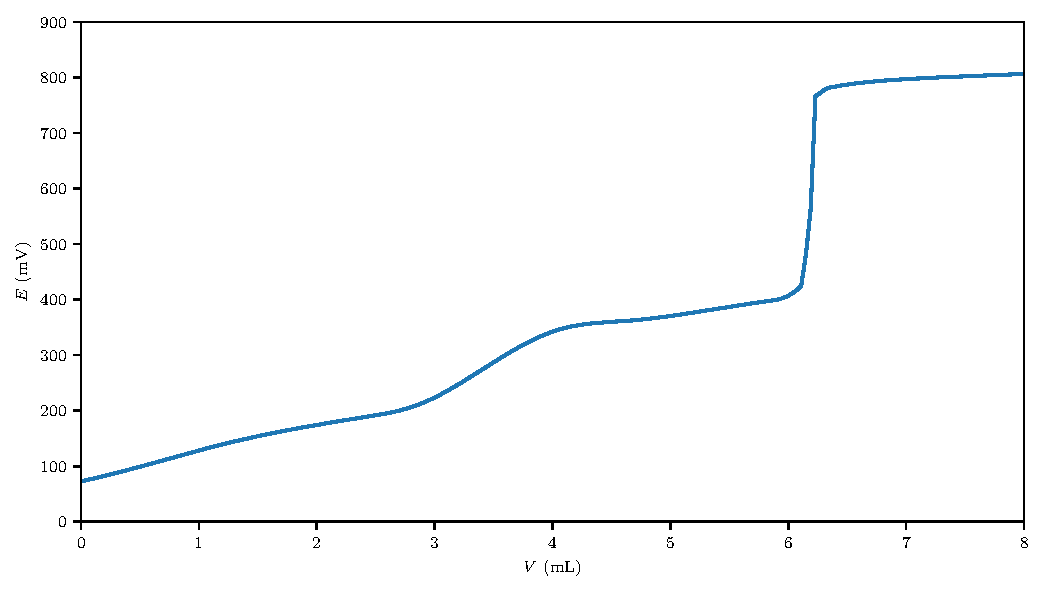
\includegraphics[width=\linewidth]{chimiePC/gene/dosage_redox.pdf}\vspace{-1em}
    \caption{Dosage potentiométrique de la solution par les ions cérium Ce$^{4+}$.}
\end{figure}

\question En déduire la valeur du produit de solubilité de l'iodure de plomb. 

\question Discuter l'intérêt de se placer en milieu chlorure pour ce dosage.
\end{questions}

\paragraph{Données : } potentiels standards $E^\circ$ dans les CNTP
\begin{center}\begin{tabularx}{.7\linewidth}{rCCC}
    \hline
    & $\mathrm{{IC\ell_2^-}_{(aq)} \,/\, {I_2}_{(aq)}}$ & $\mathrm{{I_2}_{(aq)} \,/\, {I^-_{}}_{(aq)}}$ & $\mathrm{{Ce^{4+}}_{(aq)} \,/\, {Ce^{3+}}_{(aq)}}$ \\
    $E^\circ$ (V) & 1,15 & 0,62 & 1,44 \\ \hline\hline 
\end{tabularx}
\end{center}

On note: $e^\circ = \dfrac{RT}{\scr{F}} \ln10 = 59$ mV.

\end{exercise}

\begin{solution}

\begin{questions}
\questioncours
 On considère un couple redox $Ox/Red$ tel que $Ox + ne^- = Red$ (1).
 
 On suppose que l'oxydant peut précipiter selon l'équilibre Ox + mX $\rightleftarrows OxX_{m(s)}$ avec $K_s=[Ox]\times[X]^m$
 
 On considère le nouveau couple redox $OxX_m/Red$ tel que $OxX_m + ne^- = Red + mX $   (2).
 
 La formule de Nerst donne $E_1 = E^\circ(Ox/Red) + \frac{0,06}{n}log(\frac{[Ox]}{[Red]})$ et $E_2 = E^\circ(OxX_m/Red) + \frac{0,06}{n}log(\frac{1}{[Red][X]^m})$.
 
A l'équilibre entre toutes ces espèces, les potentiels sont égaux. Cela donne donc $E^\circ(OxX_m/Red) = E^\circ(Ox/Red) - \frac{0,06}{n}pK_s $

Ainsi, lorsque l'oxydant peut précipiter, le potentiel standard du nouveau couple est abaissé et l'oxydant est donc moins réactif. De la même manière, lorsque le réducteur peut précipiter, on montre que le potentiel standard du nouveau couple augmente de $\frac{0,06}{n}pK_s$ par rapport à celui du couple $Ox/Red$ ce qui signifie également que le réducteur est moins réactif. 


\question I$^-$ : D.O.${} = -$I

I$_2$ : D.O.${} = 0$

IC$\ell_2^-$ : C$\ell$ est plus électronégatif que I donc son D.O. est de $-$I. On a donc $x-2\times1 = -1$ d'où D.O.${} = +$I.

\question La première réaction de dosage est
\begin{equation}
    \mathrm{2I^- + 2Ce^{4+} \longrightarrow I_2 + 2Ce^{3+}}, \tag{1}
\end{equation}
dont la constante est
$$\log(K_1) = 2 \times\dfrac{E^\circ\qty\big(\mathrm{Ce^{4+} / Ce^{3+}}) - E^\circ\qty\big(\mathrm{I_2 /I^-})}{e^\circ} = 27,3.$$

\`A l'équivalence, $\mathrm{[I^-]} \times V_\text{tot} = \mathrm{[Ce^{4+}]} \times V_\text{eq1}$, d'où $V_\text{eq1} = 2,0$ mL. 

Or, le bécher contenant Ce$^{3+}$, I$_2$ et C$\ell^-$, si on continue d'ajouter des ions cérium(IV), le diiode formé va réagir avec les ions Ce$^{4+}$, selon la réaction
\begin{equation}
    \mathrm{I_2 + 2Ce^{4+} + 4 C\ell^- \longrightarrow 2 IC\ell_2^- + 2Ce^{3+}}, \tag{2}
\end{equation}
avec
$$\log(K_2) = 2 \times\dfrac{E^\circ\qty\big(\mathrm{Ce^{4+} / Ce^{3+}}) - E^\circ\qty\big(\mathrm{IC\ell_2^- /I_2})}{e^\circ} = 9,70,$$
et à la deuxième équivalence, $\mathrm{[I_2]} \times V_\text{tot} = \dfrac{1}{2} \times \mathrm{[Ce^{4+}]} \times \qty\big(V_\text{eq2} - V_\text{eq1})$. Or I$_2$ est formé par la première réaction de dosage donc [I$_2$]=$\frac{[\text{I}^-]}{2}$. On a donc $V_\text{eq2} = 2 \times V_\text{eq1} = 4,0$ mL.

\question On utilise deux électrodes : une électrode de mesure (en général en platine, métal inerte puisque toutes les espèces sont en solution) et une électrode de référence (électrode au calomel saturé par exemple).

\question Dans la solution saturée, 
$$\mathrm{PbI_2 \rightleftarrows Pb^{2+} + 2I^-},$$
avec [Pb$^2+] = s$ et [I$^-] = 2s$. On a donc $K_s$=[Pb$^{2+}$]$\times$[I$^-]^2 = 4s^3$.

D'après la courbe de dosage de la solution, $V_\text{eq2} = 6,6$ mL donc $V_\text{eq1} = 3,3$ mL.

On a donc [I$^-] = 3,2 \times 10^{-3}$ mol$\cdot$L$^{-1}$.

D'où $K_s = 1,6 \times 10 ^{-8}$.

\question On remarque sur la courbe de dosage que la première équivalence n'est pas très lisible. La détermination du produit de solubilité a été faite par exploitation de la deuxième équivalence.


En l'absence des ions chlorure, seule la première équivalence aurait eu lieu et le dosage aurait été peu exploitable.

Par ailleurs, l'utilisation d'acide chlorhydrique concentré permet d'éviter la formation d'hydroxydes de plomb.

\end{questions}


\end{solution}
















% Niveau :      PCSI *
% Discipline :  Chimie Orga I
% Mots clés :   Spectrométrie UV-visible, Réactions acidobasiques

\begin{exercise}{Pile à combustible au méthanol}{2}{PCSI}
{Chimie générale,\'Electrochimie,Oxydoréduction,Pile à combustible}{bermu}

\noindent\textsl{Cet exercice étant proche du cours, une large autonomie et des remarques critiques sont attendues.}

On constitue une pile en solution aqueuse dans laquelle le méthanol liquide est dissous dans l’eau. Il est oxydé en dioxyde de carbone gazeux à l’une des électrodes, tandis que le dioxygène gazeux est réduit en eau à l’autre. L’électrolyte est une solution aqueuse d’acide sulfurique.Les deux électrodes sont séparées par une membrane poreuse, que l’on supposera imperméable au méthanol mais perméable à l’acide sulfurique.

\begin{questions}
\questioncours Détailler le fonctionnement de cette pile à combustible :
\begin{parts}
    \part faire un schéma conventionnel de la pile (le méthanol sera placé à gauche) ;
    \part détailler les demi-réactions qui ont lieu à chaque électrode ainsi que l'équation bilan ;
    \part justifier la polarité des électrodes, les nommer, et donner le sens conventionnel du courant ;
    \part proposer un matériau pour les électrodes en argumentant ;
\end{parts}

\question Donner l’expression littérale du potentiel de chaque électrode.

\question Exprimer la constante d’équilibre $K^\circ$ de la réaction de fonctionnement de la pile en fonction des potentiels standard des couples (relation à démontrer).

\question La pile débite un courant $I = 50$ mA pendant $t = 2$ heures. Quelle masse de méthanol a été consommée?

\question Un des problèmes techniques actuels est l’oxydation incomplète du méthanol en acide méthanoïque. Écrire cette demi-réaction d’oxydoréduction. \\
Comment modifie-t-elle la quantité d’électricité produite par une quantité donnée de méthanol consommée?

\question Un second problème est le passage du méthanol à travers la membrane qui sépare les deux compartiments de la pile. En quoi ce passage est-il gênant?

\end{questions}

\paragraph{Données} dans les CNTP :
\begin{itemize}
    \item Masses molaires en g$\cdot$mol$^{-1}$ : H 1 ; C 12; O 16 ;
    \item Constante de Faraday : $\scr{F} = 9,65 \times 10^4$ SI ;
    \item On note: $e^\circ = \dfrac{RT}{\scr{F}} \ln10 = 59$ mV.
\end{itemize}


\end{exercise}

\newpage

\begin{solution}
\begin{questions}
\questioncours $\mathrm{M_{(s)}}$ étant le métal de la pile, le schéma conventionel est donné ci dessous :
\begin{parts}
    \part\hspace{-.6em}{\bfseries\sffamily -- Q\,1.3}
\begin{EnvUplevel}
    %\setlength{\dashlinegap}{2pt}
    \centering
    \begin{tabularx}{.98\linewidth}{c|CC|c}
        $\Big.\mathrm{M_{(s)}}$ & $\mathrm{MeOH_{(aq)}, H^+_{(aq)}, {SO_4^{2-}}_{(aq)}}$ & $\mathrm{H^+_{(aq)}, {SO_4^{2-}}_{(aq)}}$ & $\mathrm{M_{(s)}}$  \\
        Anode & \'Ectrolyte & \'Electrolyte & Cathode \\
        $(-)$ & \multicolumn{2}{c|}{$\underset{\text{H}^+\text{, courant}}{\longrightarrow}$} & $(+)$ \\
        \multicolumn{2}{l}{$\mathrm{MeOH_{(aq)} + H_2O \longrightarrow {CO_2}_{(g)} + 6 {H^+}_{(aq)} + 6 e^-}$} &
        \multicolumn{2}{r}{$\mathrm{\dfrac{1}{2} {O_2}_{(g)}  + 2 {H^+}_{(aq)} + 2e^- \longrightarrow {H_2O}_{(\ell)}}$} \\
        \multicolumn{4}{c}{$\text{Bilan :} \quad \mathrm{MeOH_{(aq)} + \dfrac{3}{2} {O_2}_{(g)} \longrightarrow {CO_2}_{(g)} + 2 {H_2O}_{(\ell)} }$}
    \end{tabularx}
\end{EnvUplevel}
    \stepcounter{partno}
    \part L’électrode de gauche est le siège de l’oxydation du méthanol : c’est donc l’anode. Puisqu’une oxydation a lieu, le méthanol cède des électrons dans le circuit extérieur et c'est donc le pôle négatif de la pile. Et inversement.
    
    Lorsque la pile fonctionne, la réaction évolue dans le sens direct. Il s’agit donc bien d’une oxydation du méthanol par le dioxygène. Les ions H$^+$ créés dans la solution à l’électrode de gauche circulent ensuite dans l’électrolyte où ils sont consommés à l’électrode de droite.
    \part Les espèces intervenant ici sont soit des espèces dissoutes soit des gaz. Il faut donc utiliser des électrodes inattaquables en métal noble permettant comme le platine.
\end{parts}

\question En supposant que l'on soit à l'équilibre (faibles courants) :
\begin{align*}
    E_a &= E^\circ\qty\big(\mathrm{CO_2 / CH_3OH}) + \dfrac{1}{6}e^\circ \log(\dfrac{p_\mathrm{CO_2} \mathrm{[H^+]^6}}{\mathrm{[CH_3OH]}}) &
    E_c &= E^\circ\qty\big(\mathrm{O_2 / H_2O}) + \dfrac{1}{4}e^\circ \log\qty\big(\mathrm{p_\mathrm{O_2} [H^+]^4})
\end{align*}

\question \`A l'équilibre $\Delta E = E_c - E_a = 0$. On a donc
\begin{align*}
    E^\circ\qty\big(\mathrm{O_2 / H_2O}) - E^\circ\qty\big(\mathrm{CO_2 / CH_3OH})
    &= \dfrac{1}{6}e^\circ \log(\dfrac{p_\mathrm{CO_2} \mathrm{[H^+]^6}}{\mathrm{[CH_3OH]}}) - \dfrac{1}{4}e^\circ \log\qty\big(\mathrm{p_\mathrm{O_2} [H^+]^4}), \\
    6 \times \dfrac{E^\circ\qty\big(\mathrm{O_2 / H_2O}) - E^\circ\qty\big(\mathrm{CO_2 / CH_3OH})}{e^\circ} 
    &= \log(\dfrac{p_\mathrm{CO_2} \mathrm{[H^+]^6}}{\mathrm{[CH_3OH]p_\mathrm{O_2} [H^+]^4}}) = \log K^\circ,
\end{align*}
$$\text{d'o\`u} \qquad K^\circ = 10^{6 \dfrac{E^\circ\qty\big(\mathrm{O_2 / H_2O}) - E^\circ\qty\big(\mathrm{CO_2 / CH_3OH})}{e^\circ}}.$$

\question $m_\mathrm{MeOH} = M_\mathrm{MeOH} \dfrac{n_{e^-}}{6} = \dfrac{M_\mathrm{MeOH} I t}{6\scr{F}} = 20 \text{ mg}.$

\question $\mathrm{{CH_3OH}_{(aq)} + {H_2O}_{(\ell)} \longrightarrow {COOH}_{(aq)} + 4 {H^+}_{(aq)} + 4 e^-}.$ \\
Cette réaction ne produit donc que 4 électrons, contre 6 précédement et peut donc faire chuter d'au plus 33 \% le rendement de la pile.

\question Si du méthanol traverse la membrane, il peut se retrouver oxydé directement par le dioxygène au niveau de l’électrode de droite, sans entraîner de passage de courant électrique dans le circuit extérieur. C’est donc une perte nette de méthanol, le rendement de la pile baisse...

\end{questions}
\end{solution}

\section{$E$-pH}
%%%%%%%%%%%%%%%%%%%%%%%%%%%%%%%%%%%%%%%%%%%%%%%%%%%%%%%%%%%%%%%%%%%%%%%%%%%%%%%%%%%%%%%%%%%%%%%%%%%%%%%%%%%%%%

\begin{exercise}{Diagramme $E$-pH du Zirconium}{0}{Sup}
{Diagramme E-pH}{bermu}

On demande dans cet exercice de tracer le diagramme potentiel-pH du zirconium en solution aqueuse
et de l’utiliser pour discuter de la stabilité du métal au contact de l’eau.




\paragraph{Données :}
\begin{itemize}
    \item Concentration de tracé $c_\text{tra} = \SI{1.0e-6}{mol.L{-1}}\qquad$ (corrosion)

    \item $E^\circ(\mathrm{Zr^{4+_{(aq)}}/Zr_{(s)}}) = \SI{-1,44}{V}$

    \item $\text{p}K_\text{s}(\mathrm{ZrO_{2(s)}/Zr^{4+}_{(aq)}}) = 55,1\qquad$ (en milieu basique)

    \item $\text{p}K_\text{d}(\mathrm{(HZrO_3)^-_{(aq)}/ZrO_{2(s)}}) = 4,8\qquad$ (en milieu basique)

\end{itemize}

\end{exercise}

\begin{solution}

~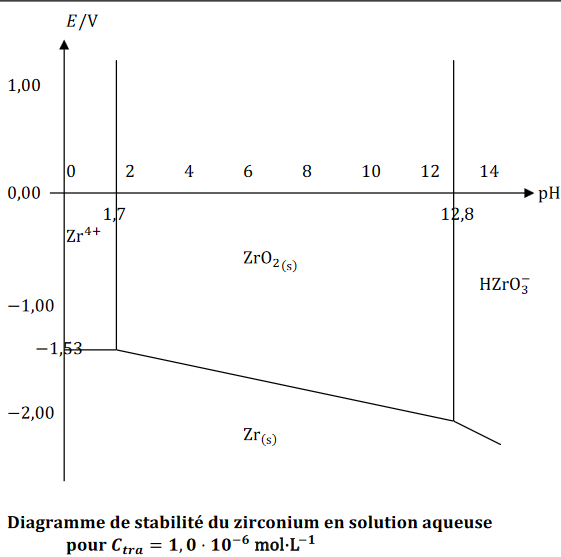
\includegraphics[]{chimie/E-pH/zirco.png}

\end{solution}
% Niveau :      PCSI *
% Discipline :  Géné
% Mots clés :   Diagrammes E-pH

\begin{exercise}{Titrage et diagramme $E$-pH}{2}{PCSI}
{Chimie générale, Réactions acidobasiques, Oxydoréduction, Diagrammes E-pH}{bermu}




\begin{questions}
\questioncours Lecture et construction de diagrammes $E$-pH.
\vspace{-1em}\begin{EnvUplevel}
Dans la figure \ref{fig:EpHS} en annexe est tracé le diagramme simplifié du soufre pour les espèces $\mathrm{S_{(s)}}$, $\mathrm{{HSO_4^-}_{(aq)}}$, $\mathrm{{SO_4^{2-}}_{(aq)}}$, $\mathrm{ {H_2S}_{(g)}}$, $\mathrm{{HS^-}_{(aq)}}$ et $\mathrm{{S^{2-}}_{(aq)}}$. \\[1ex]
\textsl{On tracera les diagrammes avec des couleurs différentes sur la figure en annexe. \\
Il ne sera exigé de calculer que les pentes de chaque frontière (tracé rapide).}
\end{EnvUplevel}
\begin{parts}
    \part En justifiant, ajouter au diagramme les domaines de prédominance / d'existence de ces espèces.
    \part Quelle est l'allure des frontières correspondant à des réactions acido-basiques ? \\
    Donner le p$K_a$ du couple $\mathrm{{HS^-}_{(aq)} / {S^{2-}}_{(aq)}}$.
    \part Quel est le potentiel standard du couple $\mathrm{{HSO_4^-}_{(aq)} / S_{(s)}}$ ?
    \part Tracer le diagramme $E$-pH de l'eau en donnant les équations des différentes frontières. \\
    \`A quoi correspondent ces trois domaines d'un point de vue chimique (mis à part les domaines de prédominance de chaque espèce) ?
    \part \`A l'aide des données, tracer le diagramme $E$-pH de l'iode.
\end{parts}

\begin{EnvUplevel}
On se propose d'étudier le protocole suivant :
\begin{enumerate}%[label={\bfseries{\itshape\alph*}\,)}]
    \item dans un bécher, introduire 20 mL d'une solution de $I_2$ à 0,1 M dans du KI saturé ;
    \item ajouter 20 mL d'une solution de soude à 2M ;
    \item introduire 20 mL d'une solution de sulfure de disodium de concentration $c \simeq 10^{-2}$ M inconnue ;
    \item chauffer avec agitation pendant 10 minutes ;
    \item après refroidissement, acidifier avec de l'acide sulfurique ;
    \item titrer avec une solution de Na$_2$S$_2$O$_3$ à 0,1 M.
\end{enumerate}

Après avoir effectué ce protocole, on trouve un volume à l'équivalence de $V_\text{éq} = 22,4$ mL.
\end{EnvUplevel}

    \question Interpréter le mode opératoire à l'aide de la figure \ref{fig:EpHS} en annexe et indiquer les réactions chimiques ayant lieu entre les différentes étapes.
    
    \question En déduire la concentration de la solution de Na$_2$S.

\end{questions}

\paragraph{Données : } potentiels standards $E^\circ$ dans les CNTP
\begin{center}\begin{tabularx}{.7\linewidth}{rCCC}
    \hline
    & $\mathrm{{I_3^-}_{(aq)} \,/\, {I^-}_{(aq)}}$
    & $\mathrm{{IO_3^-}_{(aq)} \,/\, {I_3^-}_{(aq)}}$
    & $\mathrm{{O_2}_{(g)} \,/\, {H_2O}_{(\ell)}}$ \\
    $E^\circ$ (V) & 0,53 & 1,18 & 1,23 \\
    $E^\circ / \varepsilon^\circ$ & 9,0 & 20 & 21 \\ \hline\hline 
\end{tabularx}
\end{center}

On note $\varepsilon^\circ = \dfrac{RT}{\scr{F}} \ln10 = 59$ mV.


\end{exercise}

\begin{nopagebreak}
    \exerciselabelformat{Annexe Exercice \arabic{exercise} \quad --- \quad} \textsl{\`A rendre avec la copie.}
    
    \begin{figure}[H]
        \centering
        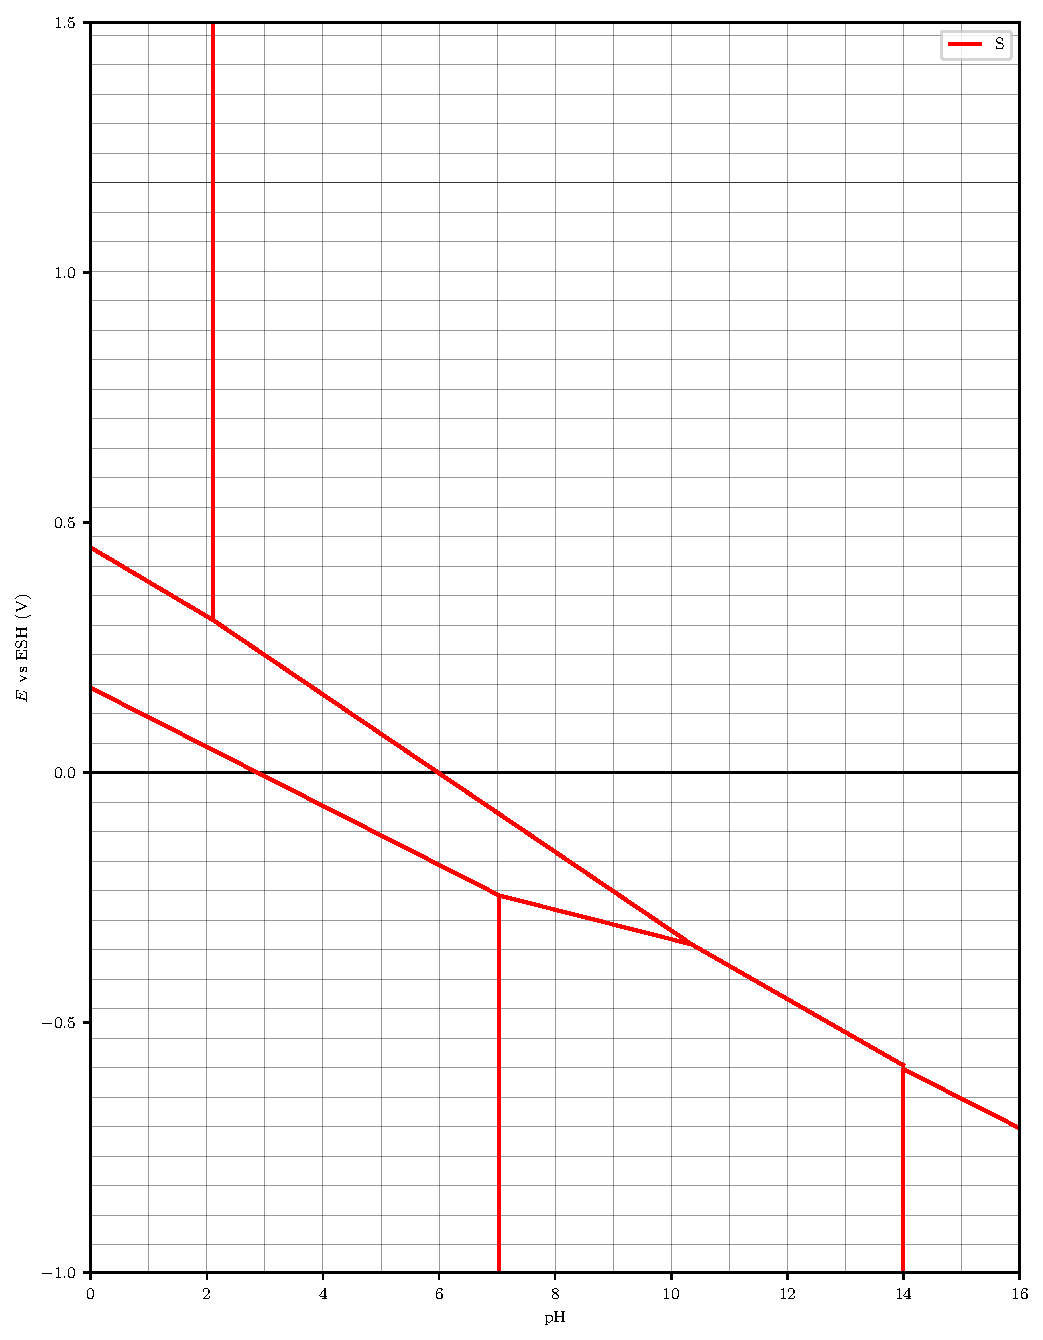
\includegraphics[width = \linewidth]{chimiePC/gene/E-pH-S.pdf}
        \caption{Diagramme $E$-pH simplifié du soufre avec une concentration de tracé de $0,1$ M. \protect\linebreak
        Le quadrillage est de $\varepsilon^\circ = 59$ mV par 1 unité de pH.}
        \label{fig:EpHS}
    \end{figure}
    
    \paragraph{Convention de tracé :}
\begin{itemize}
    \item les espèces en solution ont pour activité $c_\text{tr}/c^\circ = 10^{-1}$,
    \item les espèces gazeuses ont pour activité $p_\text{tr}/p^\circ = 10^{-2}$,
    \item les espèces solides ont pour activité $1$.
\end{itemize}

\end{nopagebreak}

\begin{solution}
\begin{questions}
\questioncours cf. le diagramme complété

\begin{parts}
    \part Les espèces du soufre ont les D.O. suivant : S$_{(s)}$ D.O. = 0 ; H$_2$S, HS$^-$, S$^{2-}$ : -II ; HSO$_4^-$ , SO$_4^{2-}$ : +VI.
    On remplit du bas vers le haut par D.O. croissant puis pour les espèces au même D.O. on place les espèces acide à gauche et basique à droite.
    
    \part Frontière verticale car pas d'échange d'électrons
   On lit sur le diagramme le pK$_a$=14.
    \part Le couple $\mathrm{{HSO_4^-}_{(aq)} / S_{(s)}}$ de demi-équation redox : HSO$_4^-$ + 7H$^+$ + 6e$^-$ = S$_{(s)}$ + 4H$_2$O.
    
    La formule de Nernst donne donc  $E = E^\circ(HSO_4^-/S_{(s)}) + \frac{0,06}{6}log([H^+]^7 \times [HSO_4^-])$.
    
    On lit sur le diagramme l'ordonnée à l'origine de la frontière entre ces deux espèces : E(pH=0) = 0,44V = $E^\circ(HSO_4^-/S_{(s)}) + 0,01\times log(10^{-1})$ d'ou $E^\circ(HSO_4^-/S_{(s)})$ = 0,45 V. 
    \part cf. cours
    Le domaine de l'eau liquide correspond au domaine de stabilité thermodynamique des espèces dans l'eau. 
    
    \part \`A l'aide des données, tracer le diagramme $E$-pH de l'iode.
\end{parts}

    \question 
    \begin{enumerate}%[label={\bfseries{\itshape\alph*}\,)}]
    \item  I$_2$ + I$^- \rightleftarrows$ I$_3^-$ 
    
    Comme KI est en excès cette réaction est quantitative on forme donc 2mmol de I$_3^-$
    
    \item On remarque qu'en milieu basique I$_3^-$ n'est pas stable et dismute en I$^-$ et IO$_3^-$ selon l'équation : 
    3I$_3^-$ + 6OH$^- \rightleftarrows$ 8I$^-$ + IO$_3^-$ + 3H$_2$O 
    
    A pH très basique, cette réaction est totale. On forme donc $\frac{2}{3}$ mmol de IO$_3^-$ et $\frac{16}{3}$ mmol de I$^-$. 
    
    \item On voit sur le diagramme que S$^{2-}$ et IO$_3^-$ ont des domaines disjoints et donc vont réagir ensemble selon l'équation : 
    
    4IO$_3^-$ + 3S$^{2-} \rightleftarrows$ 4I$^-$ + 3SO$_4^{2-}$ 
    
    Le réactif limitant est S$^{2-}$ (n(S$^{2-}) \approx$ 0,2 mmol) et donc après cette étape il reste $n = \frac{2}{3}-4\times\frac{n(S^{2-})}{3}$ $\approx$ 0,4 mmol de IO$_3^-$
    
    \item On acidifie donc la réaction de dismutation a lieu dans l'autre sens (mediamutation) (il y a toujours du KI en excès dans la solution) 
    
    8I$^-$ + IO$_3^-$ + 6H$^+$ $\rightleftarrows$ 3I$_3^-$ + 3H$_2$O
    
    IO$_3^-$ est le réactif limitant car I$^-$ est en excès, on forme donc 2-4$\times$n(S$^{2-}$) mmol de I$_3^-$.
    
    \item On dose le I$_3^-$ formé avec le thiosulfate de sodium selon l'équation :
    
    I$_3^-$ + 2S$_2$O$_3^{2-} \rightleftarrows$ 3I$^-$ + S$_4$O$_6^{2-}$ 

    \end{enumerate}
    
    \question Vu l'équation précédente, on a à l'équivalence $n_\mathrm{I_3^-} = 2-4\times [\text{S}^{2-}]\times 20 = \frac{1}{2} \mathrm{[Na_2S_2O_3]} V_\text{eq}$, d'où $c = 0,011$ M.

\end{questions}

    \begin{figure}[H]
        \centering
        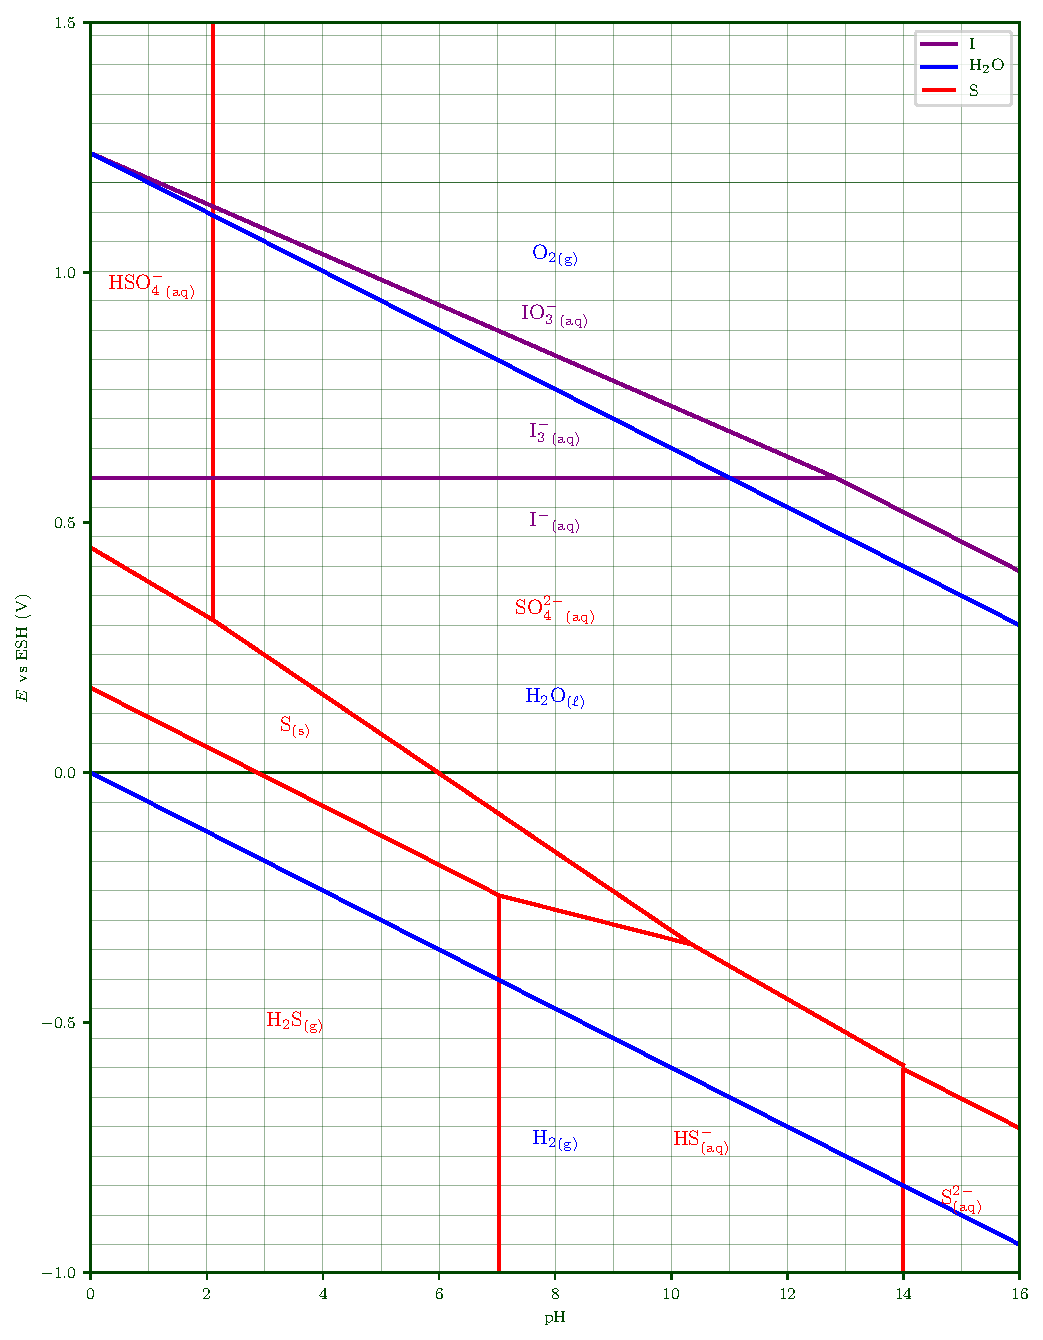
\includegraphics[width = \linewidth]{chimiePC/gene/E-pH-S-sol.pdf}
        \caption{Diagrammes $E$-pH superposés du soufre, de l'iode et de l'eau. \protect\linebreak
        Le quadrillage est de $\varepsilon^\circ = 59$ mV par 1 unité de pH.}
        \label{fig:EpHS-sol}
    \end{figure}
    
\end{solution}
% Niveau :      PCSI *
% Discipline :  Géné
% Mots clés :   Diagrammes E-pH

\begin{exercise}{Hydrométallurgie du zinc}{2}{PCSI}
{Chimie générale, Réactions acidobasiques, Oxydoréduction, Diagrammes E-pH}{bermu}

Cet exercice décrit schématiquement le processus d'extraction chimique du zinc à partir de la calcine, un minerai contenant les oxydes mixtes de cuivre (CuO, Cu$_2$O), de zinc (ZnO) et d'autres métaux. 
On se limitera par la suite à ces deux métaux.

\begin{questions}
\questioncours Lecture et construction de diagrammes $E$-pH.
\vspace{-1em}\begin{EnvUplevel}
Dans la figure \ref{fig:EpHCu} en annexe est tracé le diagramme $E$-pH du zinc pour les espèces $\mathrm{Zn_{(s)}}$, $\mathrm{{Zn^{2+}}_{(aq)}}$, $\mathrm{{Zn(OH)_2}_{(s)}}$ et $\mathrm{ {[Zn(OH)_4]^{2-}}_{(aq)}}$. \\[1ex]
\textsl{On tracera les diagrammes avec des couleurs différentes sur la figure en annexe. \\
Il ne sera exigé de calculer que les pentes de chaque frontière (tracé rapide).}
\end{EnvUplevel}
\begin{parts}
    \part En justifiant, ajouter au diagramme les domaines de prédominance / d'existence de ces espèces.
    \part Quel est le potentiel standard du couple $\mathrm{{Zn^{2+}}_{(aq)} / {Zn}_{(s)}}$ ?
    \part Tracer le diagramme $E$-pH de l'eau en donnant les équations des différentes frontières. \\
    \`A quoi correspondent ces trois domaines d'un point de vue chimique (mis à part les domaines de prédominance de chaque espèce) ?
    \part \`A l'aide des données, tracer le diagramme $E$-pH du cuivre. \\
    On pourra tout d'abord tracer en pointillés le diagramme pour les espèces de n.o. 0 et +I, puis +I et +II séparément.
\end{parts}

\begin{EnvUplevel}
    On s'intéresse maintenant au traitement de la calcine.
    
    Tout d'abord, elle est dissoute par lixiviation acide par action à chaud de l'acide sulfurique concentré.
    
    Ensuite, on introduit du zinc solide en poudre dans la solution pour éliminer les impuretés (le cuivre nottament).
    
    Enfin, les ions zinc (II) sont réduits en zinc solide par dépot sur une électrode en zinc.
\end{EnvUplevel}
    \question \'Ecrire l'équation de réaction correspondant à la lixiviation acide pour le zinc (II).
    
    \question Peut-on augmenter le pH pour précipiter et éliminer les ions cuivres de la solution ?
    
    \question Justifier donc la stratégie retenue pour éliminer le cuivre en écrivant l’équation de la réaction correspondante.
    
    \question Comment élimine-t-on ces sous-produits ?
    
    \question Expliciter la dernière étape et écrire l'équation correspondante. Proposer un matériau pour la seconde électrode.
    
    \question Pourquoi n’est-il pas possible de réaliser cette étape avec les ions cuivre et fer encore en solution ?

\end{questions}

\paragraph{Données :}

\begin{itemize}
    \item différentes espèces du cuivre dans les CNTP :

\hspace{-2em}\begin{minipage}{.68\linewidth}
Potentiels standards $E^\circ$ : \\[1em]
\begin{tabularx}{0.99\linewidth}{rCCC}
    \hline
    & $\mathrm{{Cu^{2+}}_{(aq)} \,/\, {Cu^+}_{(aq)}}$
    & $\mathrm{{Cu^{2+}}_{(aq)} \,/\, {Cu}_{(s)}}$
    & $\mathrm{{O_2}_{(g)} \,/\, {H_2O}_{(\ell)}}$ \\
    $E^\circ$ (V) & 0,16 & 0,34 & 1,23 \\
    $E^\circ / \varepsilon^\circ$ & 3 & 6 & 21 \\ \hline\hline 
\end{tabularx}
\end{minipage}
\begin{minipage}{.32\linewidth}
Produits de solubilité p$K_s$ :

\begin{tabularx}{.99\linewidth}{rCC}
    \hline
    & $\mathrm{{Cu(OH)}_{(s)}}$
    & $\mathrm{{Cu(OH)_2}_{(s)}}$ \\
    p$K_s$  & 15 & 20 \\ \hline\hline 
\end{tabularx}
\end{minipage}

    \item on note $\varepsilon^\circ = \dfrac{RT}{\scr{F}} \ln10 = 59$ mV.

    \item les oxydes métalliques et les hydroxydes métalliques seront considérés comme équivalents :
    $$\text{En milieu aqueux : } \quad \mathrm{{M_x(OH)_{2y}}_{(s)} \quad \longleftrightarrow \quad \text{En milieu sec : } {M_xO_y}_{(s)}}$$
\end{itemize}


\end{exercise}

\begin{nopagebreak}
    \exerciselabelformat{Annexe Exercice \arabic{exercise} \quad --- \quad} \textsl{\`A rendre avec la copie.}
    
    \begin{figure}[H]
        \centering
        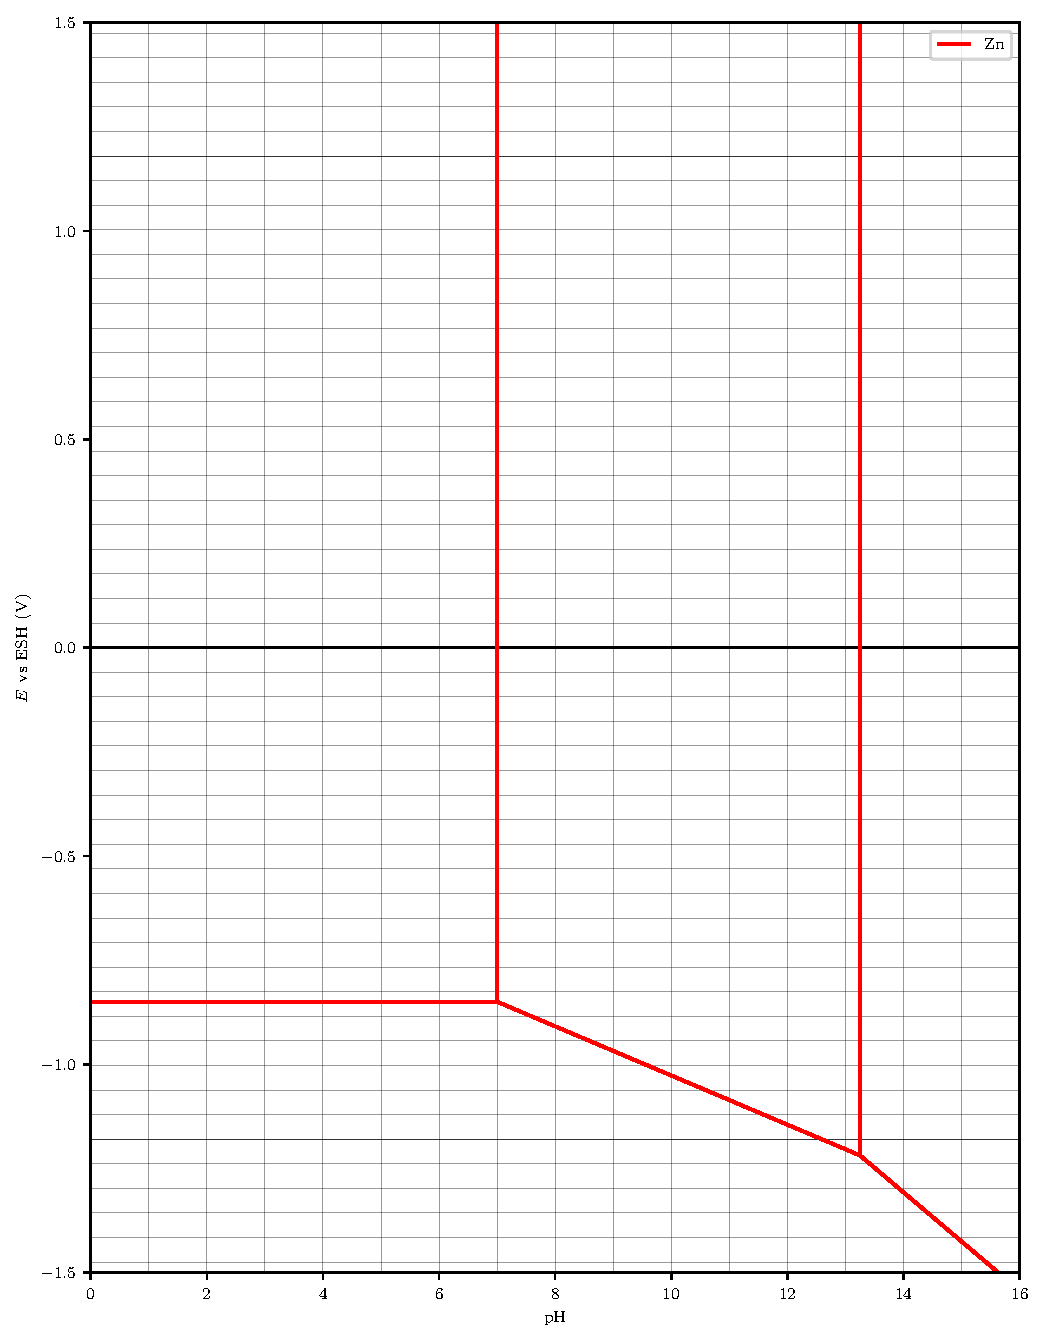
\includegraphics[width = \linewidth]{chimiePC/gene/E-pH-Zn.pdf}
        \caption{Diagramme $E$-pH du zinc avec une concentration de tracé de $10^{-2}$ M. \protect\linebreak
        Le quadrillage est de $\varepsilon^\circ = 59$ mV par 1 unité de pH.}
        \label{fig:EpHCu}
    \end{figure}
    
    \paragraph{Convention de tracé :}
\begin{itemize}
    \item les espèces en solution ont pour activité $c_\text{tr}/c^\circ = 10^{-2}$,
    \item les espèces gazeuses ont pour activité $p_\text{tr}/p^\circ = 10^{-2}$,
    \item les espèces solides ont pour activité $1$.
\end{itemize}

\end{nopagebreak}


\begin{solution}
\begin{questions}

\questioncours cf. le diagramme complété
\begin{parts}
    \part cf. cours pour la méthode.
    \part La demi-équation rédox couple $\mathrm{{Zn^{2+}}_{(aq)} / {Zn}_{(s)}}$ donne avec la relation de Nernst à la frontière $E = E^\circ + e^\circ/2 \log c_\text{tr}$, d'où $E^\circ = 0,79$ V.
    \part Le domaine central désigne le domaine de stabilité rédox de l'eau.
    \part \underline{n.o. 0 et +I :} on a  Cu$^+$ et Cu(OH) \emph{vs} Cu.
    \begin{itemize}
        \item Cu$^+$ / Cu : $E = 2 E^\circ\qty\Big(\mathrm{Cu^{2+} / Cu}) - E^\circ\qty\Big(\mathrm{Cu^{2+} / Cu^{+}}) + e^\circ \log c_\text{tr} \simeq 7 e^\circ$ ;
        \item Cu$^+$ / Cu(OH) : $\text{p}K_s = -\log c_\text{tr} + \text{p}K_e - pH$ d'où $\text{pH} = 1$ ;
        \item Cu(OH) / Cu : $\mathrm{Cu(OH) + H^+ + e^- = Cu + H_2O}$ donc pente de -0.06 V/u.pH.
    \end{itemize}
    
    \underline{n.o. +I et +II :} on a  Cu$^{2+}$ et Cu(OH)$_2$ \emph{vs} Cu$^+$ et Cu(OH).
    \begin{itemize}
        \item Cu$^{2+} / Cu^+$ : $E = E^\circ\qty\Big(\mathrm{Cu^{2+} / Cu^+}) + e^\circ \log c_\text{tr} \simeq 3 e^\circ$ ;
        \item Cu$^+$ / Cu(OH) : idem ;
        \item Cu$^{2+}$ / Cu(OH)$_2$ : $\text{p}K_s = -\log c_\text{tr} + \text{p}K_e - pH$ d'où $\text{pH} = 5$ ;
        \item Cu$^{2+}$ / Cu(OH) : $\mathrm{Cu^{2+} + H_2O + e^- = Cu(OH) + H^+}$ donc pente de +0.06 V/u.pH ;
        \item Cu(OH)$_2$ / Cu(OH) : $\mathrm{Cu(OH)_2 + H^+ + e^- = Cu(OH) + H_2O}$ donc pente de -0.06 V/u.pH.
    \end{itemize}
        
    Après tracé (en pointillés), on voit que Cu$^+$ dismute, et donc on a une frontière directe Cu$^{2+}$ / Cu à $E \simeq 5 e^\circ$.
\end{parts}

    \question $\mathrm{ZnO + 2 H^+ = Zn^{2+} + H_2O}$
    
    \question Si on augmente le pH, on va précipiter indistinctement les hydroxydes métalliques, donc ça ne marche pas.
    
    \question On voit sur le diagramme que Cu$^{2+}$ et Zn ne peuvent pas coexister. Ils vont donc réagir $$\mathrm{Cu^{2+} + Zn_{(s)} = Zn^{2+} + Cu_{(s)}}.$$
    
    \question Il suffit ensuite de filter le cuivre solide et le tour est joué.
    
    \question Il s'agit de réduire le zinc à la cathode : $\mathrm{Zn^{2+} + 2 e^- = Zn_{(s)}}$. Pour que la cathode soit l'électrode de zinc, il faut donc une anode avec un potentiel standard plus élevé comme le platine par exemple qui contrebalance avec une oxydation de l'eau
    $\mathrm{2 H_2O = O_2 + 4 H^+ + 4 e^-}$. De plus, le platine résiste au O$_2$ produit.

    \question Comme ils ont des potentiels standards plus élevés, ils réagiraient mieux et la méthode ne serait plus sélective.

\end{questions}

    \exerciselabelformat{Solution Annexe Exercice \arabic{exercise}.}
    
    \begin{figure}[H]
        \centering
        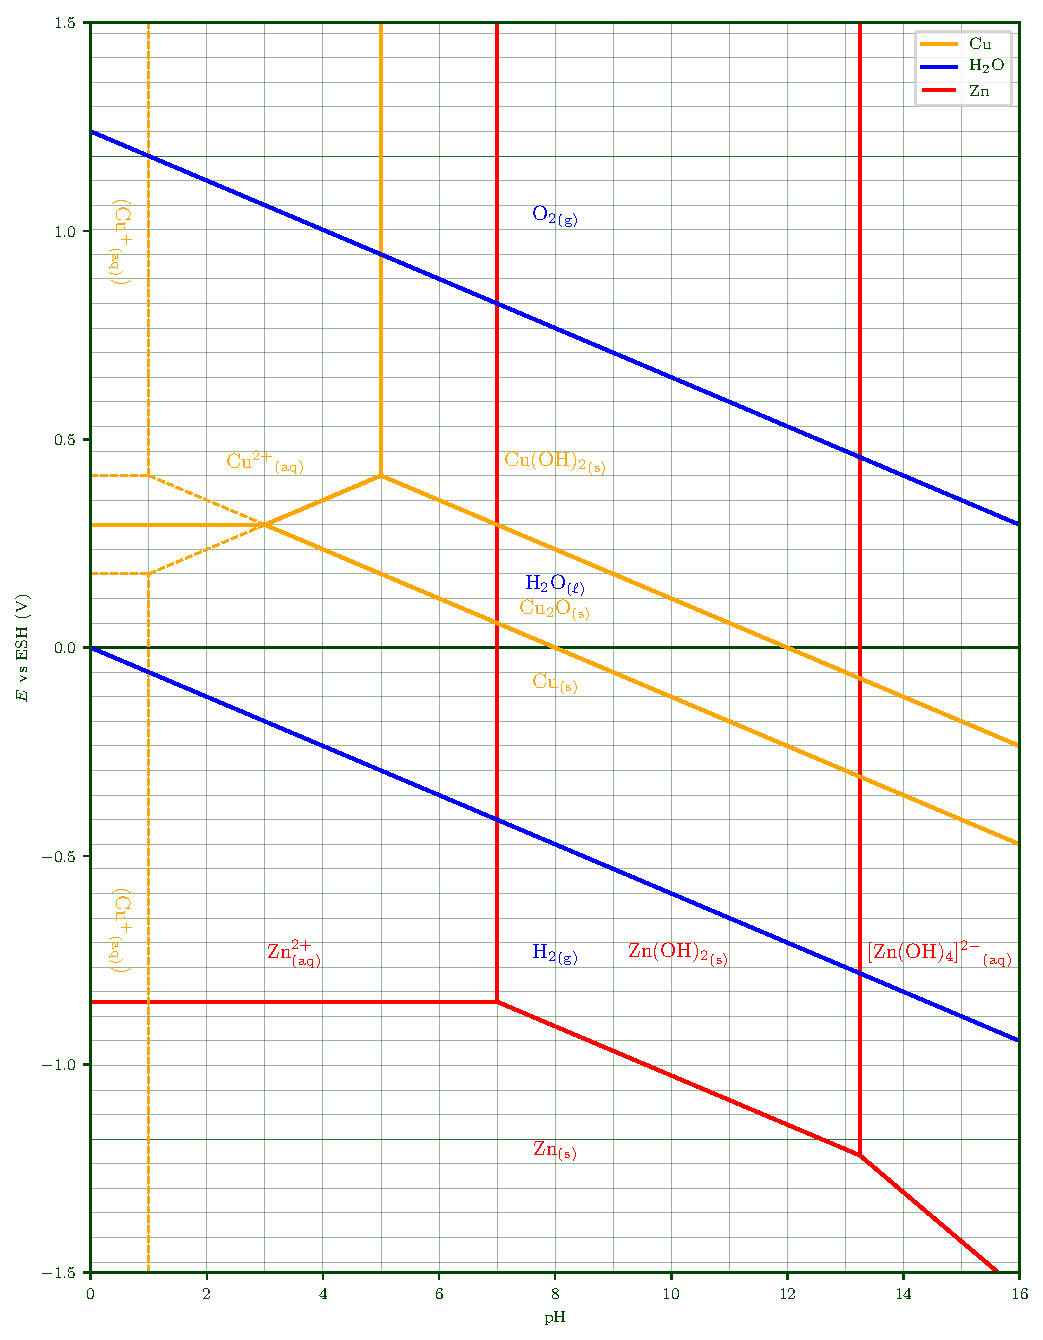
\includegraphics[width = \linewidth]{chimiePC/gene/E-pH-Zn-sol.pdf}
        \caption{Diagrammes $E$-pH superposés du cuivre, du zinc et de l'eau. \protect\linebreak
        Le quadrillage est de $\varepsilon^\circ = 59$ mV par 1 unité de pH.}
        \label{fig:EpHS-sol}
    \end{figure}

\end{solution}
\begin{exercise}{Mélange d'acide et d'eau de javel}{2}{PCSI}{Chimie générale, Oxydoréduction, Diagramme de E-pH}{chocron}

On dit souvent qu'il ne faut pas mélanger les produits ménagers, c'est en particulier le cas de l'eau de Javel  avec tout produit acide. Essayons de comprendre pourquoi. Le gaz dichlore est un gaz toxique irritant, pouvant entraîner des problèmes pulmonaires graves en cas d'inhalation. Une solution aqueuse de dichlore Cl$_{2(aq)}$ peut libérer du dichlore Cl$_{2(g)}$ gazeux. L'eau de Javel est une solution aqueuse comportant du chlorure de sodium (Na$^+$ + Cl$^-$) et de l'hypochlorite de sodium (Na$^+$ + ClO$^-$) en quantité équimolaire. Le diagramme potentiel-pH simplifié de l'élément chlore est représenté en annexe, pour les espèces chimiques HClO$_{(aq)}$, ClO$^-_{(aq)}$, Cl$_{2(aq)}$ et Cl$^-_{(aq)}$. \'A la frontière entre deux domaines, on suppose l'équirépartition en \textbf{élément} chlore. 

\begin{questions}
\question Attribuer chacun des domaines A, B, C et D à une espèce mentionnée ci-dessus.

\question En vous aidant du diagramme et des données, déterminer la valeur de C$_0$, concentration de tracé qui est la concentration totale en \textbf{élément} chlore; déterminer également la valeur du pK$_a$ du couple HClO/ClO$^-$.

\question Déterminer les pentes des frontières entre les domaines A et B, A et C ainsi que D et C. 

\question En utilisant le diagramme E-pH, prévoir l'évolution d'un mélange contenant les espèces D et C lors du passage en milieu très acide. \'A partir de quel pH observe-t-on cette réaction?

\question Donner l'équation de cette réaction et calculer sa constante d'équilibre à 298K. Comment s'appelle la réaction mise en jeu? 

\question  Conclure quant à la consigne de sécurité figurant sur les flacons d'eau de Javel de ne pas mélanger un acide avec de l'eau de Javel. 

\end{questions}
\begin{figure}[H]
    \centering
    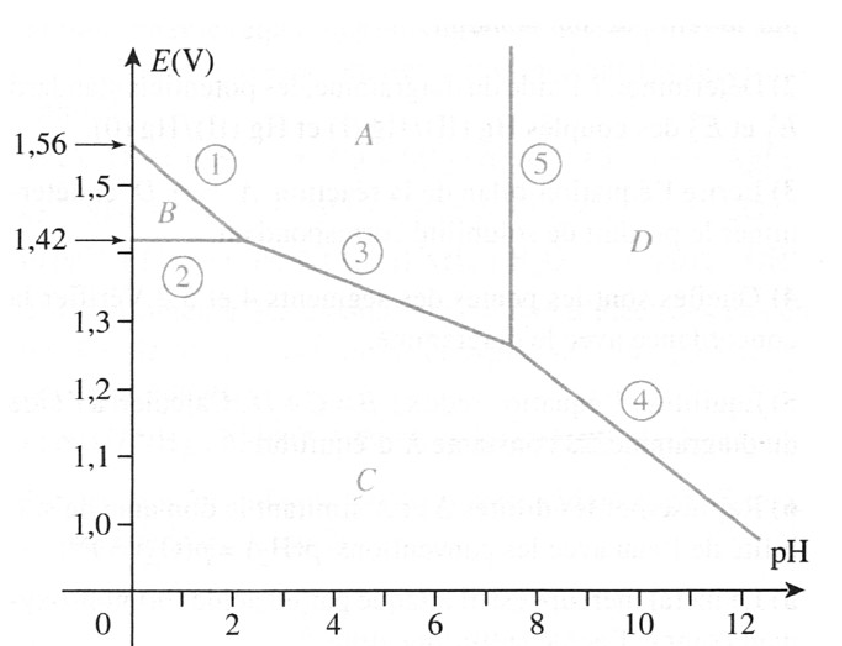
\includegraphics{chimiePC/gene/e-ph_chlore.pdf}
    \caption{Diagramme E-pH du chlore}
   
\end{figure}

\paragraph{Données : } potentiels standards $E^\circ$ dans les CNTP
\begin{center}\begin{tabularx}{.7\linewidth}{rCCC}
    \hline
    & $\mathrm{{HClO}_{(aq)} \,/\, {Cl_2}_{(aq)}}$
    & $\mathrm{{Cl_2}_{(aq)} \,/\, {Cl^-}_{(aq)}}$
    & $\mathrm{{O_2}_{(g)} \,/\, {H_2O}_{(\ell)}}$ \\
    $E^\circ$ (V) & 1,60 & 1,39 & 1,23 \\
    $E^\circ / \varepsilon^\circ$ & 27 & 24 & 21 \\ \hline\hline 
\end{tabularx}
\end{center}

On note $\varepsilon^\circ = \dfrac{RT}{\scr{F}} \ln10 = 59$ mV.


\end{exercise}


\begin{solution}

\begin{questions}
\question 
D.O. du chlore : 
Cl$_2$ : 0
Cl$^-$ : $-$I
HClO et ClO$^-$ : +I

On a donc C : Cl$^-$ ; B : Cl$_2$ ; A : HClO (espèce acide) ; D : ClO$^-$ (espèce basique).


\question  On se place à la frontière horizontale entre B et C qui correspond à la frontière entre Cl$^-$ et Cl$_2$.

La demi-équation redox correspondante est : Cl$_2$ + 2e$^-$ = 2Cl$^-$
Au niveau de cette frontière, la formule de Nernst donne : 
$E = E^\circ(Cl_{2(aq)}/Cl^-_{(aq)}) + \frac{0,06}{2}log(\frac{[Cl_2]}{[Cl^-]^2}$. 

A la frontière, l'équirépartition en chlore s'écrit : 2[Cl$_2$]=[Cl$^-$] et on a 2[Cl$_2$] + [Cl$^-$] = C$_0$.

Cela donne donc $E = E^\circ(Cl_{2(aq)}/Cl^-_{(aq)}) + 0,03log(\frac{1}{C_0})$ d'où avec les valeurs numériques des données et lue sur le diagramme, C$_0$ = 10$^{-1}$ mol.L$^{-1}$

La frontière verticale entre A et D représente l'équilibre acido-basique du couple HClO/ClO$^-$. A la frontière, on a $K_a=\frac{[ClO^-]\times[H^+]}{[HClO]}$ et [ClO$^-$]=[HClO] d'où $K_a= [H^+] $ ie $pK_a(HClO/ClO^-) = pH_{frontière}$ = 7,5.

\question La frontière entre A et B est la frontière du couple HClO/Cl$_2$ de demi-équation redox 2HClO + 2H$^+$ + 2e$^-$ = Cl$_2$ + 2H$_2$0

D'où en utilisant la formule de Nernst la pente vaut -0,06 V.

Pour A et C, on considère le couple HClO/Cl$^-$ de demi-équation HClO + H$^+$ + 2e$^-$ = Cl$^-$ + H$_2$O. La pente vaut -0,03 V.

Pour D et C, on considère le couple ClO$^-$/Cl$^-$ de demi-équation ClO$^-$ + 2H$^+$ + 2e$^-$ = Cl$^-$ + H$_2$O. La pente vaut -0,06 V.


\question Lorsque on modifie le pH d'une solution d'eau de javel (mélange de Cl$^-$ et ClO$^-$) à un pH inférieur à 2,5, HClO et Cl$^-$ n'ont plus de frontière commune donc vont réagir ensemble pour former du dichlore. A un pH inférieur à 7,5 ClO$^-$ n'est plus la forme prédominante du couple HClO/ClO$^-$.

\question Si on part d'une solution d'eau de Javel, les espèces en présence sont ClO$^-$ et Cl$^-$ donc on va considérer la réaction de ces deux espèces selon l'équation : Cl$^-$ + ClO$^-$ + 2H$^+ \rightleftarrows$ Cl$_2$ + H$_2$O. Il s'agit d'une réaction de médiamutation. 

Avec les données, on peut calculer la constante d'équilibre de la réaction 

Cl$^-$ + HClO + H$^+ \rightleftarrows$ Cl$_2$ + H$_2$O qui vaut $K_1 = 10^{\frac{E^\circ(HClO/Cl_2)-E^\circ(Cl_2/Cl^-)}{0,06}} = 10^{3,5}$ et $K$ la constante d'équilibre de la réaction avec ClO$^-$ vaut $\frac{K_1}{K_a} = 10^{3,5+7,5} = 10^{11}$.


\question On voit que la constante d'équilibre est élevée, la réaction est quantitative. Le mélange d'eau de Javel avec un acide conduit à la formation de dichlore aqueux, qui passe ensuite sous forme gazeuse. Le dichlore est un gaz très toxique, les indications sur les bouteilles sont donc tout à fait justifiées

\end{questions}
\end{solution}

\section{Courbes $i$-$E$}
%%%%%%%%%%%%%%%%%%%%%%%%%%%%%%%%%%%%%%%%%%%%%%%%%%%%%%%%%%%%%%%%%%%%%%%%%%%%%%%%%%%%%%%%%%%%%%%%%%%%%%%%%%%%%%

\begin{exercise}{Tracé de courbes $i-E$}{1}{Spé}
{Oxydoréduction, Courbes intensité potentiel}{bermu}

\textsf{Question de cours :} Tracer l’allure des courbes courant-tension pour les systèmes électrochimiques suivants (ne pas oublier les couples du solvant) :

\begin{questions}
    \question L'eau sur une électrode de platine. Système lent.
    \question $\mathrm{I_{2,(aq)}/I^-_{(aq)}}$ sur électrode de graphite ; $[\mathrm{I_2] = [\mathrm{I^-}] = \SI{0.1}{mol.L^{-1}}}$. \newline
     \hspace*{-2.1em}\textsf{Données :} $E^\circ\qty\big(\mathrm{I_{2,(aq)}/I^-_{(aq)}}) = \SI{0.54}{V}$.
    Système lent, surtensions : $\eta_\text{a} = +\SI{0.4}{V}$ et $\eta_\text{c} = \SI{-0.2}{V}$.
    \question $\mathrm{Ce^{4+}_{(aq)}/Ce^{3+}_{(aq)}}$ sur électrode de platine ; $[\mathrm{Ce^{4+}] = \SI{0.1}{mol.L^{-1}}}$, $[\mathrm{Ce^{3+}}] = \SI{0.5}{mol.L^{-1}}$. \newline
     \hspace*{-2.1em}\textsf{Données :} $E^\circ\qty\big(\mathrm{Ce^{4+}_{(aq)}/Ce^{3+}_{(aq)}}) = \SI{1.40}{V}$.
    Système rapide. $\mathrm{Ce^{4+}}$ et $\mathrm{Ce^{3+}}$ ont la même diffusivité.
\end{questions}

\end{exercise}

\begin{solution}

~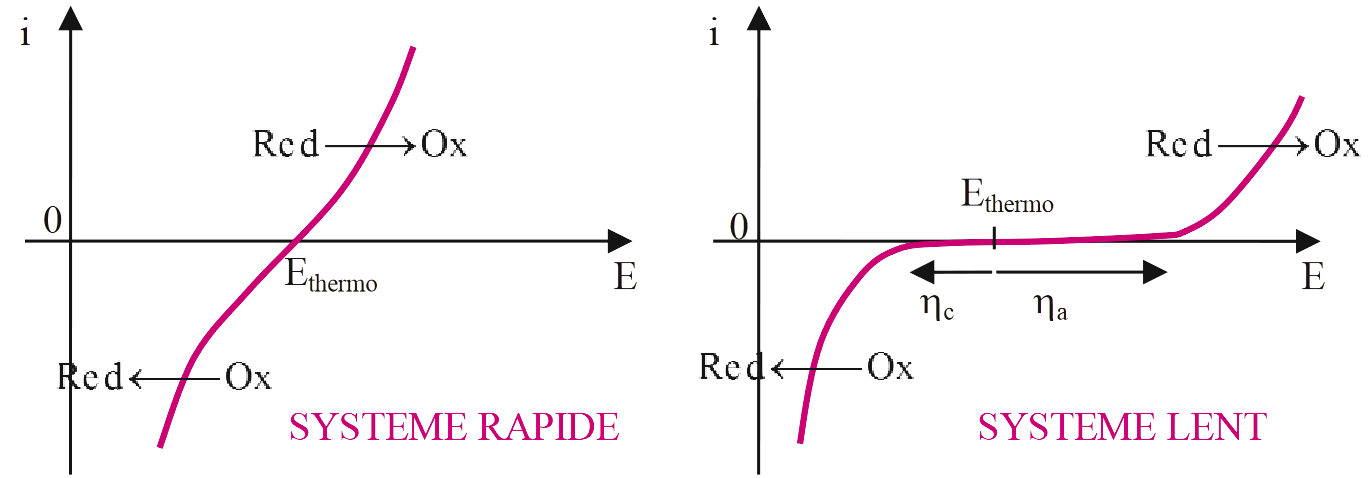
\includegraphics[width=\linewidth]{chimie/i-E/iE-cours.png}
~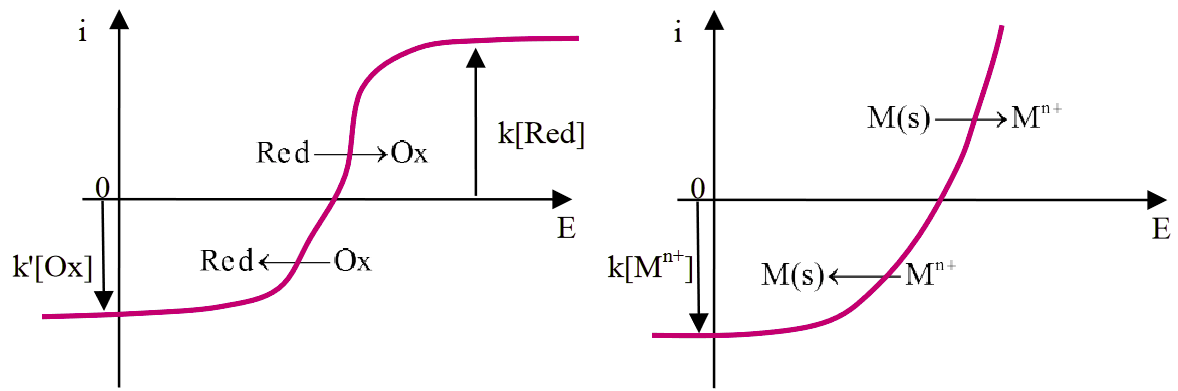
\includegraphics[width=\linewidth]{chimie/i-E/iE-cours2.png}
~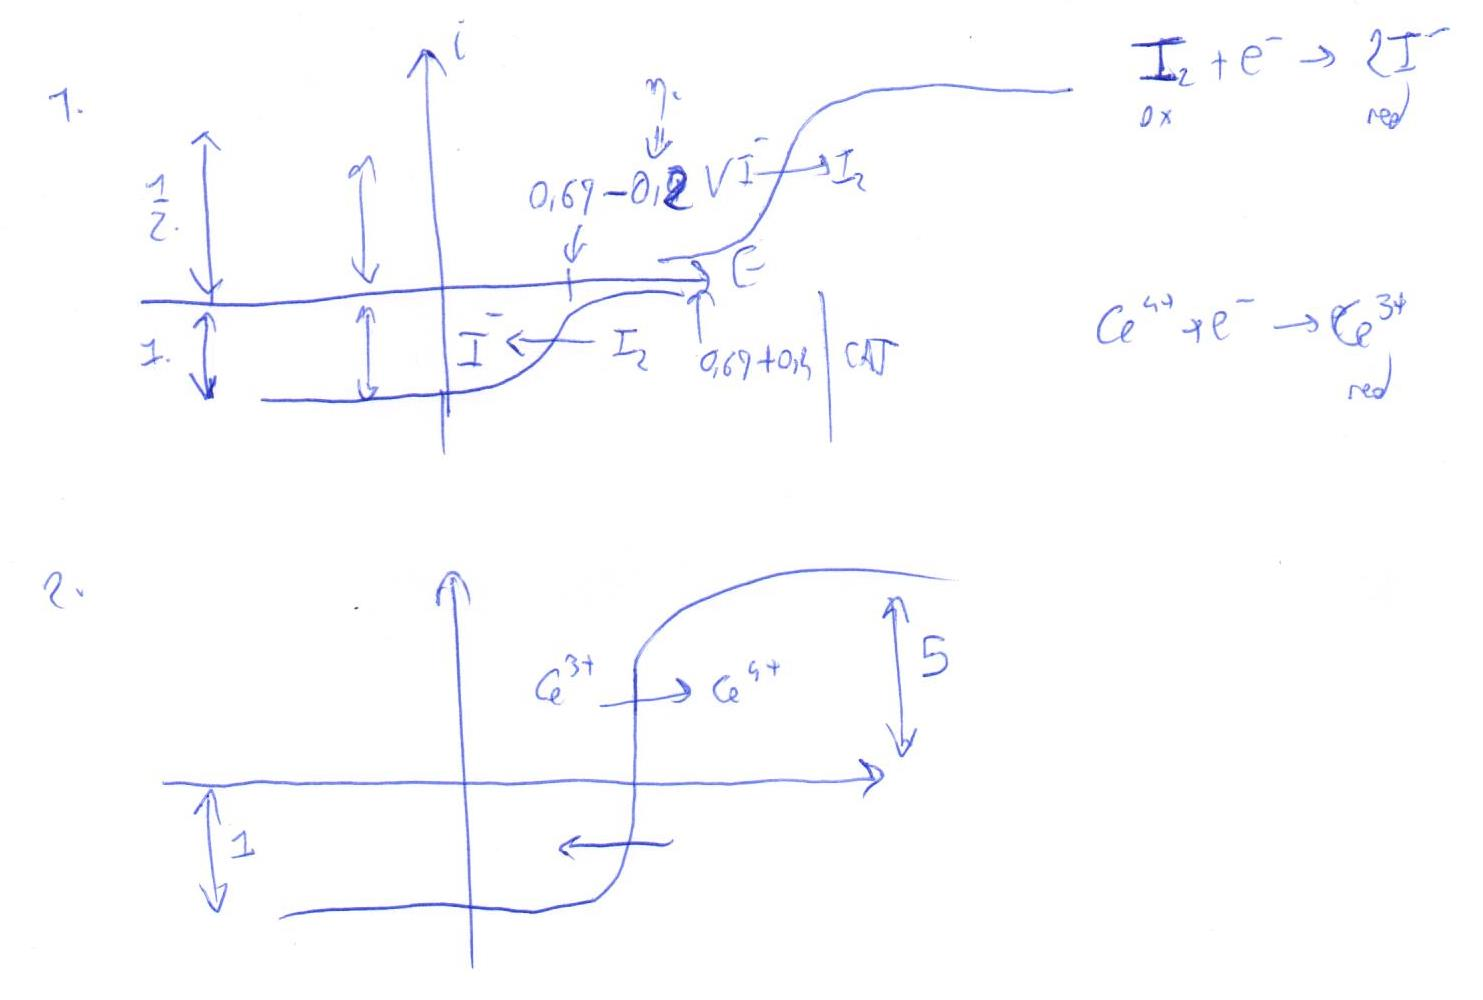
\includegraphics[width=\linewidth]{chimie/i-E/iE-corr.jpg}

\end{solution}

\begin{exercise}{Lecture de courbes $i-E$}{1}{Spé}
{Oxydoréduction, Courbes intensité potentiel}{bermu}

\textsf{Question de cours :} Interpréter quantitativement l’allure des courbes courant-tension suivantes :
\begin{questions}
    \question \hfill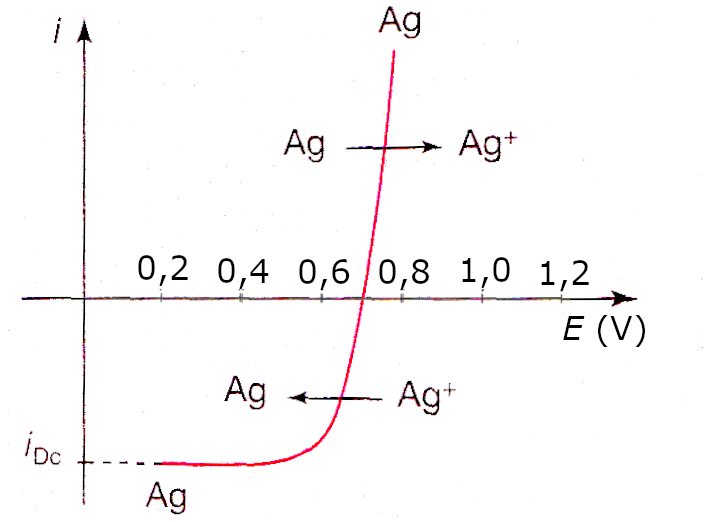
\includegraphics[valign=t,scale=1.5]{chimie/i-E/iE-2.png}\hfill ~
    
    \textsf{Données :} $[\mathrm{Ag^+}] = \SI{1e-2}{mol.L^{-1}}$, $E^\circ\qty\big(\mathrm{Ag^+_{(aq)}/Ag_{(s)}}) = \SI{0.80}{V}$.
    \question \hfill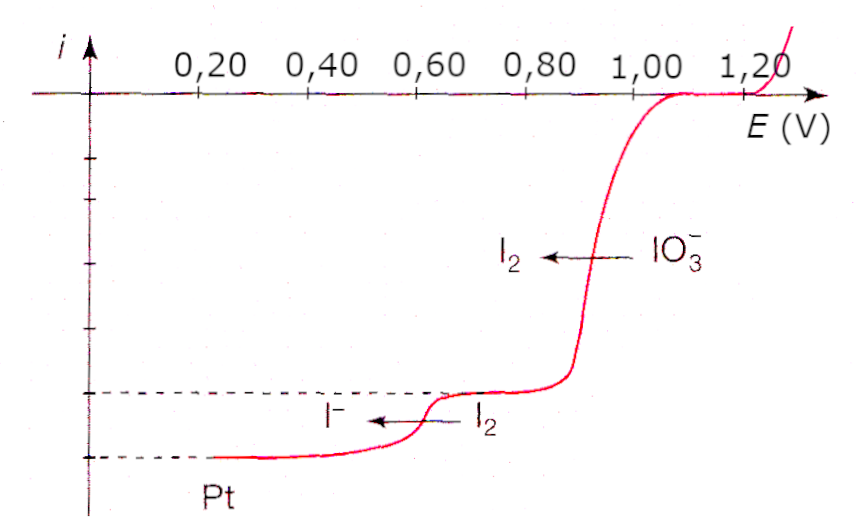
\includegraphics[valign=t,scale=1.5]{chimie/i-E/iE-1.png}\hfill ~

    \textsf{Données :} $E^\circ\qty\big(\mathrm{I_{2,(aq)}/I^-_{(aq)}}) = \SI{0.54}{V}$, $E^\circ\qty\big(\mathrm{IO^-_{3,(aq)}/I_{2,(aq)}}) = \SI{1.19}{V}$.
\end{questions}

\end{exercise}

\begin{solution}

\paragraph{Pistes :}

\begin{questions}
    \question~
        \begin{parts}
            \part Pourquoi n’observe-t-on pas de palier de diffusion anodique pour le système $\mathrm{Ag^+_{(aq)}/Ag_{(s)}}$ ?
            \part Vérifier numériquement la valeur du potentiel à l’équilibre.
            \part Ce système est-il rapide ou lent ?
        \end{parts}
    \question~
        \begin{parts}
            \part Pourquoi observe-t-on des vagues de réduction de hauteur différente ?
            \part Prévoir l’allure de la courbe d’oxydation d’une solution d’iodure sur platine.
        \end{parts}
\end{questions}

\end{solution}
%%%%%%%%%%%%%%%%%%%%%%%%%%%%%%%%%%%%%%%%%%%%%%%%%%%%%%%%%%%%%%%%%%%%%%%%%%%%%%%%%%%%%%%%%%%%%%%%%%%%%%%%%%%%%%

\begin{exercise}{Potentiel mixte}{2}{Spé}
{Oxydoréduction, Courbes intensité potentiel}{bermu}

\begin{questions}
    \questioncours Potentiel mixte.
    \uplevel{Deux électrodes, l’une de fer et l’autre de zinc plongent dans une solution de chlorure de sodium (dont le seul rôle est d’assurer la conduction électrolytique). Elles sont court-circuitées.
    
    On observe un dégagement gazeux au niveau de l’électrode de fer et l’apparition d’un précipité blanc au niveau de l’électrode de zinc.}
    \question Interpréter ces observations à l’aide de courbes intensité-potentiel et évaluer le potentiel mixte de la solution.
\end{questions}

\paragraph{Données}

\begin{itemize}
    \item $E^\circ\qty\big(\mathrm{Fe^{2+}_{(aq)}/Fe_{(s)}}) = \SI{-0.44}{V}$
    \item $E^\circ\qty\big(\mathrm{Zn^{2+}_{(aq)}/Zn_{(s)}}) = \SI{-0.76}{V}$
    \item $\text{p}K_\text{s}(\mathrm{Zn(OH)_{2(s)}/Zr^{2+}_{(aq)}}) = 17.1$
    \item surtension du couple $\mathrm{H^+_{(aq)}/H_{2(g)}}$ sur le fer $\eta = \SI{-0.2}{V}$.
\end{itemize}

\end{exercise}

\begin{solution}

\begin{questions}
    \questioncours $j=0$ ne veut pas dire équilibre thermo !

    \begin{center}
        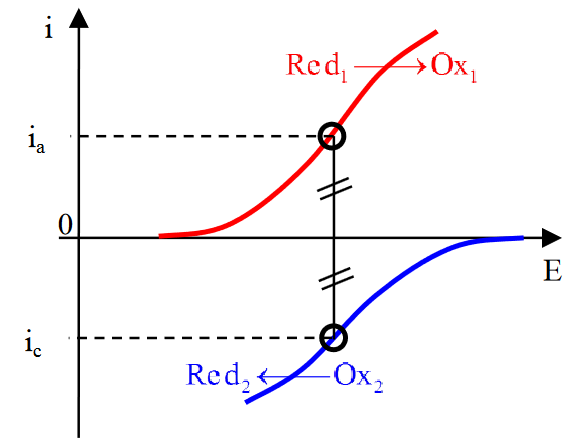
\includegraphics[scale=1.]{chimie/i-E/iE-cours3.png}
    \end{center}
    On observes spontanément un dégagement gazeux au niveau de l’électrode de fer et l’apparition d’un précipité blanc au niveau de l’électrode de zinc.
    \question Dégagement gazeux $=$ H$_2$. $\mathrm{2H^+_{(aq)} + 2 e^- \xrightarrow{Fe_{(s)}} H_{2(g)} }$.
    
    Précipité blanc $= \mathrm{Zn(OH)_{2(s)}}$. $\mathrm{Zn_{s(aq)} + 4 H_2O_{(\ell)} \xrightarrow{Zn_{(s)}} Zn(OH)_{2(s)} + 2H^+_{(aq)} + 2 e^- }$
    
~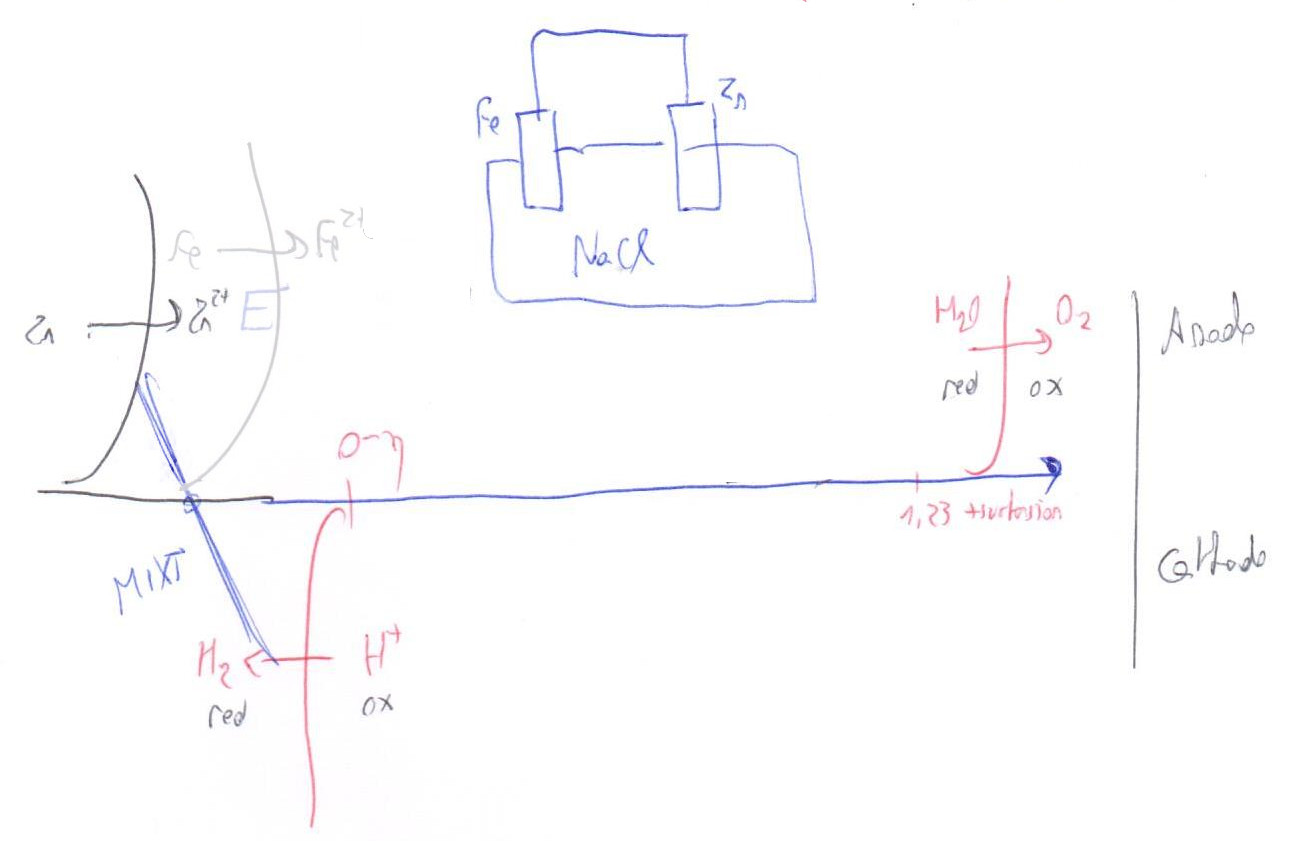
\includegraphics[width=\linewidth]{chimie/i-E/iE-corr2.jpg} 
\end{questions}

\end{solution}

%https://www.lycee-champollion.fr/IMG/pdf/td_no2_chimie_14-15.pdf

\section{Cinétique}

\begin{exercise}{Dissociation du dibrome}{1}{PCSI}
{cinetique}{lelay}

Le dibrome Br$_2$ a tendance à se dissocier en deux molécules de brome Br selon la réaction

$$ \text{Br}_2 \longrightarrow 2\, \text{Br} $$

Qui suit une cinétique d'ordre 1 en Br$_2$.

\begin{questions}

    \question Donner l'expression de la concentration en dibrome au cours du temps.
    
\end{questions}
\end{exercise}

\begin{solution}
\begin{questions}

    \question La loi est d'ordre 1, d'où
    $$ v = - \dv{\qty[\text{Br}_2]}{t} = k \qty[\text{Br}_2]$$
    d'où
    $$ \qty[\text{Br}_2](t) = \qty[\text{Br}_2]_0 e^{-kt}$$
    
\end{questions}
\end{solution}

%%%%%%%%%%%%%%%%%%%%%%%%%%%%%%%%%%%%%%%%%%%%%%%%%%%%%%%%%%%%%%%%%%%%%%%%%%%%%%%%%%%%%%%%%%%%%%%%%%%%%%%%%%%%%%

\begin{exercise}{Détemination de l'âge d'une roche}{1}{PCSI}
{cinetique}{lelay}

Lors de sa formation, une roche contenait initialement $7.22\cdot 10^{18}$~noyaux de potassium~40, un isotope du potassium de demie vie $\tau_{1/2} = 1.25\cdot 10^9$~ans.

Aujourd'hui, la même roche ne contient plus que $7.60\cdot 10^{17}$~noyaux de potassium~40.

\begin{questions}

    \question Déterminer l'âge de cette roche
    
\end{questions}
\end{exercise}

\begin{solution}
\begin{questions}

    \question Le nombre de noyaux radioactifs décroit exponentiellement (cinétique d'ordre 1)
    $$ N(t) = N_0 e^{-\lambda t}$$
    avec $\lambda = \ln 2 / \tau_{1/2} = 5.55\cdot 10^{9}$~ans ; d'où
    $$ t = -\frac1\lambda \ln\qty(\frac{N(t)}{N_0}) = 4.06 \time 10^9\text{ ans}$$
    donc 4 milliards d'année.
    
\end{questions}
\end{solution}

%%%%%%%%%%%%%%%%%%%%%%%%%%%%%%%%%%%%%%%%%%%%%%%%%%%%%%%%%%%%%%%%%%%%%%%%%%%%%%%%%%%%%%%%%%%%%%%%%%%%%%%%%%%%%%

\begin{exercise}{Décomposition du bromure de nitrosyle}{1}{PCSI}
{cinetique}{lelay}

Le bromure de nitrosyle se décompose selon la réaction suivante :
$$
\text{NOBr}_\text{(g)} = \text{NO}_\text{(g)} + \frac12\, {\text{Br}_2}_\text{(g)}.
$$
La concentration en bromure de nitrosyle a été mesuré à différentes dates :
\begin{table}[H]
    \centering
    \begin{tabular}{l|c|c|c|c|c|c}
        Temps $t$ (min)             &  0    & 6.2   & 10.8    & 14.7  & 20    & 24.6   \\
        \hline
        Concentration $c$ (mol/L)   & 0.0250    & 0.0191  & 0.0162    & 0.0144    & 0.0125    & 0.0112
    \end{tabular}
    % \caption{Caption}
    % \label{tab:my_label}
\end{table}

\begin{questions}

    \question Déterminer par la méthode intégrale l'ordre de la réaction
    
\end{questions}
\end{exercise}

\begin{solution}
\begin{questions}

    \question Il faut tracer $c = f(t)$ (ordre 0), $\ln c = f(t)$ (ordre 1) et $1/c = f(t)$ (ordre 2) et faire des régressions linéaires.
    
    On trouve des coefficients $r^2$ respectivement de 0.94089, 0.98482 et 0.99999 donc la réaction est d'ordre 2
    
\end{questions}
\end{solution}

%%%%%%%%%%%%%%%%%%%%%%%%%%%%%%%%%%%%%%%%%%%%%%%%%%%%%%%%%%%%%%%%%%%%%%%%%%%%%%%%%%%%%%%%%%%%%%%%%%%%%%%%%%%%%%

\begin{exercise}{Dégradation de l'eau oxygénée}{1}{PCSI}
{cinetique}{lelay}

Une solution d'eau oxygénée contient du peroxyde d'hydrogène H$_2$O$_2$, un produit que se décompose au cours du temps selon la réaction
$$
\text{H}_2\text{O}_2 \longrightarrow \text{H}_2 \text{O} + \frac12\, \text{O}_2
$$
qui suit une loi de vitesse d'ordre 1.

La constante cinétique $k_\text{obs}$ de cette reáction a été mesurée à différentes températures. Les résultats sont présentés dans le tableau ci dessous

\begin{table}[H]
    \centering
    \begin{tabular}{c|c}
        Température & $k_\text{obs}$ (heures$^{-1}$) \\
        20 $^o$C &  0.0065 \\
        30 $^o$C &  0.0144 \\
        40 $^o$C &  0.0276 
    \end{tabular}
    % \caption{Caption}
    % \label{tab:my_label}
\end{table}

\begin{questions}

    \question En utilisant la loi d'Arrhenius, déterminer l'énergie d'activation de la décomposition de l'eau oxygénée. 
    
\end{questions}
\end{exercise}

\begin{solution}
\begin{questions}

    \question Il faut partir de $$k_\text{obs} = A e^{-E_a/RT}$$ pour écrire
    $$
    \ln k_\text{obs} = \ln A - \frac{E_a}{R} \frac{1}{T}
    $$ et faire une régression linéaire en $\ln k_\text{obs}$ et $1/T$.
    
    On trouve $A = 1.7 \cdot 10^7$ h$^{-1}$ et $E_a = 53$~kJ/mol.
    
\end{questions}
Les données sont extraites du mémoire d'Émilie Savage, IMPACT DE LA TEMPÉRATURE SUR LA DÉGRADATION DU PEROXYDE D’HYDROGÈNE LORS DE LA RÉHABILITATION IN SITU D’AQUIFÈRES CONTAMINÉS.
\end{solution}

% Niveau :      PCSI *
% Discipline :  Chimie Orga
% Mots clés :   Stéréochimie

\begin{exercise}{De la cinétique à l'équilibre}{2}{PCSI}
{Transformationn de la matière,Cinétique,Arrhénius}{bermu}

\begin{questions}
\questioncours \'Evolution de la constante de vitesse chimique avec les concentrations et la température.

\begin{EnvUplevel}
    On étudie la réaction d'isomérisation suivante
    $$\mathrm{\underset{\textsfbf{A}}{{CH_3-CO-CH_3}_{(aq)}} \quad\overset{1}{\underset{-1}{\rightleftharpoons}}\quad \underset{\textsfbf{B}}{{CH_3-C(OH)=CH_2}_{(aq)}}},$$
    pour laquelle la constante d'équilibre est $K^\circ$. On introduit initialement \textsfbf{A} avec une concentration $c_0$.
\end{EnvUplevel}

\question Justifier la qualification d'isomérisation.

\question Quel est l'avancement volumique maximal de la réaction $1$, $\xi_\text{max}$ ?

\question Donner les équations cinétiques des vitesses $v_1$ et $v_{-1}$ des deux réactions 1 et $-1$ en fonction des constantes de vitesses $k_1$ et $k_{-1}$.

\question En déduire un système sous la forme
$$\left\lbrace\mqty{\displaystyle\dv{[\textsfbf{A}]}{t} = f\qty\big([\textsfbf{A}],[\textsfbf{B}])\\[2ex] \displaystyle\dv{[\textsfbf{B}]}{t} = g\qty\big([\textsfbf{A}],[\textsfbf{B}])}\right.$$

\question Justifier qualitativement que la concentration totale est constante et donner cette constante. Montrer que le système d'équation précédent vérifie cette propriété.

\question En déduire que l'on peut séparer le système sous la forme
$$\left\lbrace\mqty{\displaystyle\dv{[\textsfbf{A}]}{t} = -\dfrac{1}{\tau}[\textsfbf{A}] + \text{cte}_1 \\[2ex] \displaystyle\dv{[\textsfbf{B}]}{t} = -\dfrac{1}{\tau}[\textsfbf{B}] + \text{cte}_2}\right.$$
On précisera l'expression de $\tau$, cte$_1$ et cte$_2$. Que représente $\tau$ ?

\question On se place à $t \gg \tau$. Décrire l'état final, et en particulier donner l'avancement volumique final $\xi_\text{f}$, le quotient de réaction final $Q_\text{f}$ et les vitesses de réaction $v_1$ et $v_{-1}$. Commentaire ?

\question En déduire une relation entre $K^\circ$, $k_1$ et $k_{-1}$ et lui donner un sens chimique. 

\question Comment évolue $K^\circ$ en fonction de la température ?



\end{questions}


\end{exercise}

% Niveau :      PCSI *
% Discipline :  Chimie Orga
% Mots clés :   Stéréochimie

\begin{exercise}{Modèle clé-serrure de Michaelis--Menten}{3}{PCSI}
{Transformationn de la matière,Cinétique,Arrhénius}{bermu}

\begin{questions}
\questioncours Profil d'énergie potentielle d'une réaction chimique et influence d'un catalyseur.

\begin{EnvUplevel}
     En 1913, à partir de résultats expérimentaux, Victor Henri, Leonor Michaelis et Laure Menten proposent pour une réaction enzymatique
     $$\mathrm{\underset{\text{substrat}}{S} \overset{E}{=} \underset{\text{produit}}{P}},$$
     le mécanisme clé-serrure suivant :
     \begin{figure}[H]
         \centering
         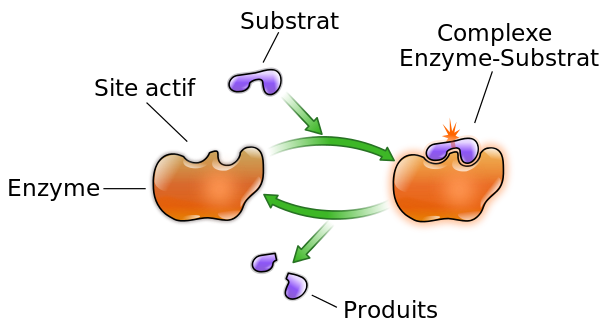
\includegraphics[width=0.6\linewidth]{chimie/cinetique/cinetique.png}
         \caption{Mécanisme clé-serrure}
         \label{fig:my_label}
     \end{figure}
     
     On notera [E$^\ast$] la concentration du complexe enzyme-substrat, [E] la concentration d'enzyme, [S] la concentration du substrat et [P] la concentration du produit.
     
\end{EnvUplevel}

\question En vous inspirant de la Figure 1, proposer un mécanisme en deux étapes modélisant la réaction. \\ On considérera que les deux étapes, notées 1 et 2, sont élémentaires, réversibles et de constantes $k_1$, $k_{-1}$ et $k_2$, $k_{-2}$.
    
\question Caractériser l'équilibre de la réaction S = P.

\question En notant $v(t)$ la vitesse de production de P, donner la loi de vitesse dans l'AEQS en fonction des concentrations [S]$_t$ et [P]$_t$, de la concentration totale en enzyme [E]$_\text{tot}$ = [E]$_t$ + [E$^\ast$]$_t$ et des constantes cinétiques.

\paragraph{Aide :} on pourra chercher la valeur de $\dfrac{[\text{E}]}{[\text{E}]^\ast}$ dans le cadre de l'AEQS et en déduire $\dfrac{[\text{E}]}{[\text{E}]_\text{tot}}$ et  $\dfrac{[\text{E}^\ast]}{[\text{E}]_\text{tot}}$.

\question \'Evaluer les vitesses maximales dans le sens S $\rightarrow$ P et P $\rightarrow$ S.

\question En déduire que la loi de vitesse peut s'écrire
$$v(t) = \dfrac{k_1 v^\text{max}_{\text{S} \rightarrow \text{P}}[\text{S}] - k_{-2} v^\text{max}_{\text{P} \rightarrow \text{S}}[\text{P}]}{k_1(c_\text{s} + [\text{S}]) + k_{-2}(c_\text{p} + [\text{P}])},$$
où $c_\text{s}$ et $c_\text{p}$ sont les deux constantes dites de Michaelis dont on donnera les expressions.

Donner un sens chimique à cette expression.

\uplevel{On se place désormais dans le cas où l'étape donnant le produit est perçue comme irréversible.}

\question Interpréter chimiquement ce que cela signifie à partir de la loi de vitesse de la question 4 et de la constante d'équilibre de la question 3.

\question En déduire une expression simplifiée de la loi de vitesse de la question 6, dépendant uniquement de $v^\text{max}_{\text{S} \rightarrow \text{P}}$ et $c_\text{s}/[\text{S}]$.

\question Etablir une méthode graphique pour évaluer $v_\text{max}$ et $c_\text{s}$.

\end{questions}

\end{exercise}


% Niveau :      PCSI *
% Discipline :  Cinétique
% Mots clés :   Stéréochimie

\begin{exercise}{Modèle épidémiologique}{2}{PCSI}
{Transformationn de la matière,Cinétique}{bermu}

\begin{questions}
\questioncours Notion d'ordre d'une réaction : ordre global, ordre apparent, ordre initial.

\begin{EnvUplevel}
    On s'intéresse à la cinétique de la propagation d'un pathogène dans une population. Pour cela, on divise la population en quatre catégories :
    \begin{itemize}
        \item \textsfbf{S} : les personnes susceptibles d'être contaminées ;
        \item \textsfbf{E} : les personnes exposées au pathogène, en période d'incubation ;
        \item \textsfbf{I} : les personnes infectées et donc contagieuses ;
        \item \textsfbf{R} : les personnes rétablies.
    \end{itemize}
    
    On écrit par ailleurs les processus d'exposition (1), d'infection (2) et de rétablissement (3) comme :
    $$\text{(1)}\quad\textsfbf{S} + \textsfbf{I} \xrightarrow[]{\ \beta\ } \textsfbf{E} + \textsfbf{I}, \qquad\qquad
    \text{(2)}\quad\textsfbf{E} \xrightarrow[]{\ \sigma\ }
      \textsfbf{I} , \qquad\qquad
      \text{(3)}\quad\textsfbf{I}\xrightarrow[]{\ \gamma\ }
      \textsfbf{R} $$
\end{EnvUplevel}

\question Interpréter les réactions (1), (2) et (3) d'un point de vue chimique.

\question En supposant les ordres courants de chaque réaction égaux à la molécularité de chaque espèce, donner la vitesse de chaque réaction en fonction des dérivées $\dv{[\textsfbf{S}]}{t}$, ...

\question En faisant l'approximation des états quasi-stationnaire sur \textsfbf{E}, donner la 


\end{questions}


\end{exercise}


% Niveau :      PCSI *
% Discipline :  Chimie Orga
% Mots clés :   Stéréochimie

\begin{exercise}{Horloge chimique}{3}{PCSI}
{Transformationn de la matière,Cinétique,Arrhénius}{bermu}

\begin{questions}
\questioncours Approximation de l’étape cinétiquement déterminante. \\ On illustrera par un exemple.

\begin{EnvUplevel}
     Hans Heinrich Landolt découvre en 1886 une réaction qu'il qualifie d'horloge chimique.
     
     Partant d'une solution contenant des ions iodure (I$^-$, $\mathrm{[I]_i} = 10$ mmol) et thiosulfate (S$_2$O$_3^{2-}$, $\mathrm{[S_2O_3^{2-}]_i} = 10$ mmol) et de l'amidon (noté L, $\mathrm{[L]_i} = 100$ mmol), on ajoute de l'eau oxygénée (H$_2$O$_2$) acidifiée (H$^+$). Les variations de volumes sont négligées.
     
     On observe que la solution, limpide initialement, devient violette au bout de $\tau = 5$ secondes.
     
     Il se produit trois réactions :
     \begin{enumerate}[label={\quad(\arabic*)}]
         \item $\mathrm{3 I^- + H_2O_2 + 2 H^+ \quad\longrightarrow\quad I_3^- + 2 H_2O}$, lente, $K^\circ_1 = 10^{30}$ ;
         \item entre I$_3^-$ et S$_2$O$_3^{2-}$ qui produit I$^-$ et S$_4$O$_6^{2-}$, rapide, $K^\circ_2 = 10^{50}$ ;
         \item $\mathrm{I_3^- + L \quad\rightleftharpoons\quad [I_3L]^-}$, qui colore la solution en violet, rapide, $K^\circ_3 = 10^{20}$.
     \end{enumerate}
\end{EnvUplevel}

\question Initialement, à $t=0$, seule la réaction (1) se produit.
\begin{parts}
    \part Que veux-t-on dire par 'la réaction est totale et lente' ? Donner des critères quantifiant ces deux affirmations.
    \part Sachant que la concentration en eau oxygénée et en ions H$^+$ est très grande (on précisera devant quoi), donner une expression simplifiée de la loi de vitesse de la réaction 1. On pourra considérer qu'elle est d'ordre effectif 1.
    \part Donner la concentration de $\mathrm{[I_3^-]_1}(t)$ en fonction du temps, et des données du problème, compte tenu uniquement de la réaction (1). Estimer  la constante de vitesse de réaction effective $k^\text{eff}_1$ ainsi que la vitesse de réaction initiale $v^\text{i}_1$ à l'aide des données du problème.
\end{parts}

\question On considère qu'il s'est initialement formé par la réaction (1) une petite quantité $\varepsilon$ de I$_3^-$. \\
Il est immédiatement consommé par les réactions (2) et (3). 
\begin{parts}
    \part Équilibrer l'équation de réaction de (2).
    \part En précisant les hypothèses utilisées et en les justifiant par des calculs rigoureux, donner l'état final du système à l'instant $t$.
    
    % \textsfbf{Aide :} considérer le rapport des avancements volumiques $\xi_2^\text{i,éq}/\xi_3^\text{i,éq}$ à l'instant initial.
    
    \part Comment évolue donc le système initialement ? Donner l'évolution (totale) de $\mathrm{[I^-]}(t)$, $\mathrm{[I_3^-]}(t)$ et $\mathrm{[S_2O_3^{2-}]}(t)$ en fonction des données du problème et de $v_1^\text{i}$.
\end{parts}


\end{questions}

\end{exercise}


\section{Thermodynamique chimique}
% Niveau :      PCSI *
% Discipline :  Chimie Orga I
% Mots clés :   Spectrométrie UV-visible, Réactions acidobasiques

\begin{exercise}{Raffinage du nickel par le procédé Mond}{2}{PC,MP}
{Thermochimie, Affinité, Déplacement d'équilibre}{bermu}


    Du nickel de très haute pureté peut être obtenu par l’intermédiaire du nickel carbonyle (tétracarbonylenickel) Ni(CO)$_4$. Ce complexe se forme à température modérée et pression ordinaire par action du monoxyde de carbone gazeux CO$_\text{(g)}$ sur des pastilles de nickel Ni$_\text{(s)}$.
    Aucun autre métal n’est susceptible de réagir dans les mêmes conditions.
    
    Après séparation, le nickel carbonyle est décomposé selon la réaction inverse pour donner du métal de haute pureté.

\begin{questions}
    \question \'Ecrire l'équation de réaction, avec une stoechiométrie 1 pour le nickel.
    \question À l’aide des données thermodynamiques fournies, établir, en fonction de la température $T$, les expressions de l’enthalpie libre standard de la réaction, dans les domaines de température 0--43$^\circ$C et 43--200$^\circ$.
    
Pouvait-on prévoir le signe du coefficient de $T$ dans l’expression de l’enthalpie libre standard de réaction ?

    \question Tracer le graphe de l’enthalpie libre standard de réaction $\Delta_\text{r}G^\circ$ en fonction de la
température $T$.

Quelle est la température d’inversion de l’équilibre ?

    \question Quelle est la variance d’un système à l’équilibre constitué de nickel solide, de monoxyde de carbone et de nickel carbonyle gazeux ? Quel est l’effet sur ce système d’une augmentation de pression à température constante ?
    
    \question Quelle est la variance d’un système à l’équilibre constitué de nickel solide, de monoxyde de carbone et de nickel carbonyle liquide ? Quel est l’effet sur ce système d’une augmentation de température à pression constante ?
    
    \question Pour une pression totale de 1 bar, à quelle température sera-t-il judicieux de se placer pour former le nickel carbonyle et le séparer facilement des impuretés, peu volatiles, contenues dans le métal ? On choisira entre 20 $^\circ$C, 40 $^\circ$C, 50 $^\circ$C, 100 $^\circ$C, 150 $^\circ$C ou 200 $^\circ$C.
    
    \question Quelle température conviendra le mieux pour décomposer le nickel carbonyle sous une pression totale de 1 bar ? On choisira entre 20 $^\circ$C, 40 $^\circ$C, 50 $^\circ$C, 100 $^\circ$C, 150$^\circ$C.
    
    \paragraph{Données :} dans les conditions standard.
    
    \'Ebullition de Ni(CO)$_4$ : $T_\text{vap} = 43$ $^\circ$C, $\Delta_\text{vap}H^\circ = 30$ kJ$\cdot$mol$^{-1}$.
    
    Dans les CNTP :
    \begin{center}
\begin{table}[H]
    \qquad\begin{tabular}{r|cccc}
        Espèce & $\mathrm{Ni_{(s)}}$ & $\mathrm{CO_{(g)}}$ & $\mathrm{Ni(CO)_{4 (\ell)}}$ \\ \hline\hline
        $\Delta_\text{f}H^\circ$ (kJ$\cdot$mol$^{-1}$) & --- & $-111$ & $-632$ \\
        $S_m^\circ$ (J$\cdot$mol$^{-1}\cdot$K$^{-1}$) & $30$ & $198$ & $320$ \\ \hline
    \end{tabular}
\end{table}
    \end{center}
\end{questions}

\end{exercise}


% Niveau :      PCSI *
% Discipline :  Chimie Orga I
% Mots clés :   Spectrométrie UV-visible, Réactions acidobasiques

\begin{exercise}{Oxydation du soufre}{2}{PC,MP}
{Thermochimie, Affinité, Déplacement d'équilibre}{bermu}

    Nous allons nous intéresser au passage du dioxyde de soufre SO$_{2 \text{(g)}}$ au trioxyde de soufre SO$_{3 \text{(g)}}$ par l'action de l'oxygène O$_{2 \text{(g)}}$. Ce passage se fait essentiellement au contact d’un catalyseur spécifique, le pentaoxyde de vanadium V2O5.

\begin{questions}
    \question \'Ecrire l'équation de réaction, avec une stoechiométrie 1 pour le dioxygène.
    
    \question Calculer son enthalpie standard de réaction et son entropie standard de réaction à $T = 300$ K et en déduire l'expression de l’enthalpie libre standard de réaction pour toute température $T$.
    
    \question Quelle est la température d’inversion de l’équilibre ? Préciser l’expression numérique de $\ln K^\circ(T)$ pour toute température ($K^\circ$ désigne la constante d’équilibre).
    
    \uplevel{Les industriels travaillent vers $T = 430$ $^\circ$C sous $p = P^\circ = 1$ bar avec un léger excès de dioxygène
provenant de l’air par rapport à la quantité stoechiométrique 2 SO$_2$ pour 1 O$_2$. Nous allons interpréter ces choix.}

    \question Partons de $\lambda$ moles de dioxygène pur et de $1 - \lambda$ moles de dioxyde de soufre. Dresser un tableau d’avancement et donner la relation liant à l’équilibre le paramètre $\lambda$, l’avancement $\xi$, la constante d’équilibre $K^\circ$ et la pression totale $p$.
    
    \question À $T$ et $p$ fixées, pour quelle valeur de $\lambda$ a-t-on un avancement $\xi$ maximal ?
    
    \uplevel{Nous supposons que nous partons désormais des proportions stoechiométriques : 2 mol de dioxyde de soufre pour 1 mol de dioxygène et que l’équilibre est atteint.}
    
    \question Quelle est l’influence d’un ajout de diazote à $T$ et $p$ constantes sur l’état d’équilibre ?

    \question Conclure sur la meilleure composition théorique du mélange initial.
    
    \question Comment interpréter le choix de la pression atmosphérique par les industriels ?
    
    \paragraph{Données :} dans les CNTP
    \begin{center}
\begin{table}[H]
    \qquad\begin{tabular}{r|cccc}
        Espèce & $\mathrm{SO_{2 (g)}}$ & $\mathrm{SO_{3 (g)}}$ & $\mathrm{O_{2 (g)}}$ \\ \hline\hline
        $\Delta_\text{f}H^\circ$ (kJ$\cdot$mol$^{-1}$) & $-297$ & $-396$ & --- \\
        $S_m^\circ$ (J$\cdot$mol$^{-1}\cdot$K$^{-1}$) & $248$ & $257$ & $205$ \\ \hline
    \end{tabular}
\end{table}
    \end{center}
\end{questions}

\end{exercise}

% Niveau :      PCSI *
% Discipline :  Chimie Orga I
% Mots clés :   Spectrométrie UV-visible, Réactions acidobasiques

\begin{exercise}{Déplacements d'équilibre}{2}{PC,MP}
{Thermochimie, Affinité, Déplacement d'équilibre}{bermu}


\begin{questions}
    \questioncours Loi de Van't Hoff : interprétation et démonstration.
    
\begin{EnvUplevel}
    Dans cet exercice, on étudie le critère d'évolution d'une réaction sous la forme générale
    \begin{equation}
        \sum_i\nu_i A_i = 0, \tag*{de constante $K^\circ(T)$}
    \end{equation}
    où les $\nu_i$ sont les coefficients stoechiométriques écrits algébriquement avec la convention
    $$\left\lbrace\begin{array}{ll}
        \nu_i > 0 & \text{pour les espèces produites, \emph{i.e.} les produits ;}  \\
        \nu_i < 0 & \text{pour les espèces consommées, \emph{i.e.} les réactifs ;}  \\
        \nu_i = 0 & \text{pour les espèces inertes.}  \\ 
    \end{array}\right.$$
    
    On rappelle la définition de l'opérateur de Lewis $$\Delta_\text{r}X = \qty(\pdv{X}{\xi})_{P,T},$$
    $\xi$ étant l'avancement de la réaction et $X$ une grandeur quelconque ($G$, $H$, $S$, $V$...)
\end{EnvUplevel}
    \question \textsf{Quelques rappels}
    \begin{parts}
        \part Rappeler les relations entre $\Delta_\text{r}G^\circ$ et $K^\circ(T)$ ; entre $\Delta_\text{r}G$, $K^\circ$ et $Q$.
        \part Rappeler le critère d'évolution d'une réaction vers l'équilibre avec $Q/K^\circ$ d'une part et $\Delta_\text{r}G$ d'autre part, et montrer que ces deux critères sont équivalents.
    \end{parts}
    
    \uplevel{La réaction est constituée d'une phase aqueuse en contact avec une phase gazeuse. On partage d'un coté les $\nu_{i,\text{g}}$ gazeux, les $\nu_{i,\text{aq}}$ aqueux et les $\nu_{i,\ast}$ constitué des corps purs et du solvant.}
    
    \question Montrer qu'on peut décomposer $\Delta_\text{r}G$ de la manière suivante
    \begin{equation}
        \Delta_\text{r}G = \Delta_\text{r}G^\circ + RT\ln Q_\text{g} + RT\ln Q_\text{aq} + RT\ln Q_\ast. \tag{$\star$}
    \end{equation}
        On précisera les expressions de $Q_\text{g}$ en fonction de $x_{i,\text{g}} = n_{i,\text{g}}/n_\text{tot,g}$, $\nu_{i,\text{g}}$ et $P$ ; de $Q_\text{aq}$ en fonction de $c_{i,\text{aq}}$, $\nu_{i,\text{aq}}$ et enfin de $Q_\ast$.
    
    \question Partant de l'équilibre, on change la température $T \mapsto T + \dd{T}$ à pression constante.
    \begin{parts}
        \part Que vaut $\Delta_\text{r}G$ à l'équilibre ?
        \part Montrer que seule la variation de $\Delta_\text{r}G^\circ(T)$ contribue à changer $\Delta_\text{r}G(T)$ dans la relation $(\star)$.
        \part En déduire
        $$\qty(\pdv{\Delta_\text{r}G}{T})_{P,n_i,\text{éq}} = -\dfrac{\Delta_\text{r}H^\circ}{T},$$
        interpréter le sens chimique de cette relation.
    \end{parts}
    
    \question Partant de l'équilibre, on change la pression $P \mapsto P + \dd{P}$ à température constante.
    \begin{parts}
        \part Quel est le seul terme qui varie dans la relation $(\star)$ ?
        \part En déduire
        $$\qty(\pdv{\Delta_\text{r}G}{P})_{T,n_i,\text{éq}} = \dfrac{\Delta_\text{r}n_\text{tot,g}RT}{P} = \Delta_\text{r}V,$$
        où on a noté $\Delta_\text{r}n_\text{tot,g} = \sum_{i,\text{g}} \nu_i$ (justifier cette notation), interpréter le sens chimique de cette relation.
        
        Ce principe est connu sous le nom de Le Châtelier.
    \end{parts}
    
    \question Partant le l'équilibre, on augmente le volume de la solution $V_\text{sol} \mapsto V_\text{sol} + \dd{V_\text{sol}}.$
    \begin{parts}
        \part Réécrire $Q_\text{aq}$ en fonction des $n_i$, de $V_\text{sol}$, $n_{i,\text{aq}}$ et $\nu_{i,\text{aq}}$.
        \part En déduire
        $$\qty(\pdv{\Delta_\text{r}G}{V_\text{sol}})_{T,P,n_i,\text{éq}} = \dfrac{\Delta_\text{r}n_\text{tot,aq}RT}{V_\text{sol}},$$
        où on a noté $\Delta_\text{r}n_\text{tot,aq} = \sum_{i,\text{aq}} \nu_i$ (justifier cette notation), interpréter le sens chimique de cette relation.
    \end{parts}
        
    \question Conclure quant à un principe modérateur générique en chimie.
    
\end{questions}

\end{exercise}

% Niveau :      MP
% Discipline :  Thermo
% Mots clés :   Premier principe, second principe

\begin{exercise}{Premier principe chimique}{1}{MP}
{Chimie, Thermodynamique, Premier principe}{bermu}


\begin{questions}
    \questioncours Premier principe dans un système à composition variable. \\ Enthalpie standard de formation. Loi de Hess (démonstration).
    
\uplevel{Dans cet exercice, on étudie la réaction de combustion du méthane $CH_4$.}
    
    \question \'Equilibrer la réaction suivante et déterminer son enthalpie standard de réaction. Cette réaction est-elle exothermique ou endothermique ?
    $$\mathrm{{CH_4}_{(g)} + {O_2}_{(g)} \longrightarrow {CO_2}_{(g)} + {H_2O}_{(\ell)}}$$
    
\uplevel{Pour un système adiabatique, la température de flamme $T_\text{f}$ est la température telle que toute la chaleur de réaction est utilisée pour chauffer le système.}
    \question Déterminez la température de flemme de cette réaction.
    
\uplevel{En réalité, la combustion se fait dans l'air.}
    \question Rappeler les trois composants majoritaires de l'air ainsi que la proportion $\beta$ de O$_{2(g)}$.
    \question Si on appelle ${c^\circ_p}'$ la capacité thermique des gaz de l'air autres que O$_2$, quelle est la nouvelle expression de $T_\text{f}$ ?
    \question Dans le cas le taux de réaction n'est pas complet $\alpha$, quelle est la nouvelle expression de $T_\text{f}$ ? 
    
\end{questions}

\paragraph{Données :} enthalpies standard de formation et capacités thermiques isobares à 295K.

\begin{table}[H]
    \qquad\begin{tabular}{r|ccccc}
        Espèce & $\mathrm{CH_{4 (g)}}$ & $\mathrm{O_{2 (g)}}$ & $\mathrm{CO_{2 (g)}}$ & $\mathrm{H_2O_{(\ell)}}$ & Autres gaz \\ \hline\hline
        $\Delta_\text{f}H^\circ$ (kJ$\cdot$mol$^{-1}$) & $-74,4$ & --- & $-394$ & $-286$ & --- \\
        $c_p^\circ$ (J$\cdot$mol$^{-1}\cdot$K$^{-1}$) & $36,0$ & $29,4$ & $46,7$ & $33,6$ & $29,3$ \\ \hline
    \end{tabular}
\end{table}
\end{exercise}
\begin{solution}

\begin{questions}
    \questioncours Premier principe dans un système à composition variable. \\ Enthalpie standard de formation. Loi de Hess (démonstration).
    
\uplevel{Dans cet exercice, on étudie la réaction de combustion du méthane $CH_4$.}
    
    \question exothermique
    
\uplevel{Pour un système adiabatique, la température de flamme $T_\text{f}$ est la température telle que toute la chaleur de réaction est utilisée pour chauffer le système.}
    \question Hypothèse : tous les reactifs ont reagi
    
\uplevel{En réalité, la combustion se fait dans l'air.}
    \question 20\% O2
    \question zoom zoom zang
    \question zim zim zoom
    
\end{questions}

\end{solution}


\begin{exercise}{Second principe chimique}{1}{MP}
{Chimie, Thermodynamique, Second principe}{bermu}

\begin{questions}
    \questioncours Second principe dans un système à composition variable dans la formulation de De Donder.
    
\uplevel{Dans cet exercice, on étudie la réaction d'isomérisation de deux énantiomères R et S de l'acide aminé alanine.}
    
    \question Justifier qualitativement que les deux molécules ont des potentiels chimiques identiques : $\mu^\ast_\textsc{r} = \mu^\ast_\textsc{s} = \mu^\ast$. Donner en fonction du potentiel chimique standard de l'alanine $\mu^\circ$ le potentiel chimique de l'alanine en proportion $\alpha$.
    
    \question Initialement, on introduit $n_0$ moles d'un seul énantiomère pur (R par exemple). Il est observé une réation de racémisation :
    $$\mathrm{R \leftrightharpoons S}.$$
    Justifier qualitativement qu'un tel mélange est idéal.
    
    \question Exprimez la différence l'enthalpie libre molaire $\Delta G_\text{m}(\eta,T)$ du système par rapport à l'état initial en fonction de l'avancement relatif $\eta$ de la réaction, de la température $T$ et de $\mu^\circ(T)$.
    
    \question Quel est l'état d'équilibre final ? Donner $\Delta G_\text{m,tot}(T)$. En quoi cette expression est-elle universelle ?
    
\end{questions}

\end{exercise}
\begin{solution}

\begin{questions}
    \questioncours Second principe dans un système à composition variable dans la formulation de De Donder.
    
\uplevel{Dans cet exercice, on étudie la réaction d'isomérisation de deux énantiomères R et S de l'acide aminé alanine.}
    
    \question $\mu = \mu^0 + RT \ln(\alpha)$
    
    \question C LA MEME
    
    \question Puisque $G = G(R) + G(S)$,
    \begin{align*}
        \Delta G &= G_{final} &- G_{init} \\
        &= \eta (\mu_0 + RT\ln(\eta)) + (1-\eta)(\mu_0 + RT\ln(1-\eta)) &- 1(\mu_0 + RT\ln(1)) \\
        &= \eta RT\ln(\eta)  + (1-\eta) RT \ln(1-\eta)&
    \end{align*}
    
    \question $G_\text{m,tot}(T) = -RT\ln(2)$ ($\eta= 1/2$ pour minimiser)
    
\end{questions}

\end{solution}


\begin{exercise}{Potentiel chimique}{1}{MP}
{Chimie, Thermodynamique, Potentiel chimique}{bermu}


\begin{questions}
    \questioncours Potentiel chimique : définition et expression dans différent systèmes.
    
\uplevel{Dans cet exercice, on étudie le potentiel chimique de l'eau.}
    \question Déterminer l'effet d'une augmentation de pression de $\Delta P = 100$ bar sur le potentiel chimique de l'eau.
    
    \question Déterminer l'effet d'une augmentation de température de $\Delta T = 100$ K sur le potentiel chimique de l'eau
    \begin{parts}
        \part En supposant constantes les grandeurs thermodynamiques en fonction de la température.
        \part En prenant en compte de la dépendance des grandeurs thermodynamiques à la température avec la capacité thermique de l'eau.
    \end{parts}
    Comparer les deux résultats.

\end{questions}

\paragraph{Données :} la plupart est supposée connue pour l'eau, mais on pourra demander si besoin.

\end{exercise}

\begin{solution}
    $V^\circ_m = 18 \cdot 10^{-6}$ m$^3\cdot$mol$^-1$, $\Delta\mu^\ast_P = 180$ J$\cdot$mol$^{-1}$ \\
    $S^\circ_m = 70$ J$\cdot$K$^-1\cdot$mol$^-1$, $\Delta\mu^\ast_T = -7$ kJ$\cdot$mol$^{-1}$ \\
    $c^\circ_{pm} = 75$ J$\cdot$K$^-1\cdot$mol$^-1$, ${\Delta\mu^\ast_T}' = -8,14$ kJ$\cdot$mol$^{-1}$
    

\begin{questions}
    \questioncours Potentiel chimique : définition et expression dans différent systèmes.
    
\uplevel{Dans cet exercice, on étudie le potentiel chimique de l'eau.}
    \question $\mu^* = \mu^0 + V_m^* (P-P^0)$
    
    \question Déterminer l'effet d'une augmentation de température de $\Delta T = 100$ K sur le potentiel chimique de l'eau
    \begin{parts}
        \part $\pdv{\mu}{T} = S_m^*$
        \part $\dd{H} = T\dd{S}$ donc $\pdv{S}{T} = \frac{c_p}{T}$
    \end{parts}
    Comparer les deux résultats.
    
\end{questions}


\end{solution}
%% Niveau :      PCSI *
% Discipline :  Chimie Orga I
% Mots clés :   Spectrométrie UV-visible, Réactions acidobasiques

\begin{exercise}{Les hydrures du bloc $p$}{2}{MPSI}
{Atomistique,Classification périodique, Structure électronique}{bermu}

\begin{questions}
    
    \questioncours En introduisant dans le détail les concepts utilisés, commenter l'évolution des caractéristiques physiques des hydrures des éléments du bloc $p$ présentés dans la figure et la table ci-dessous.
\end{questions}

    \begin{figure}[H]
        \centering
        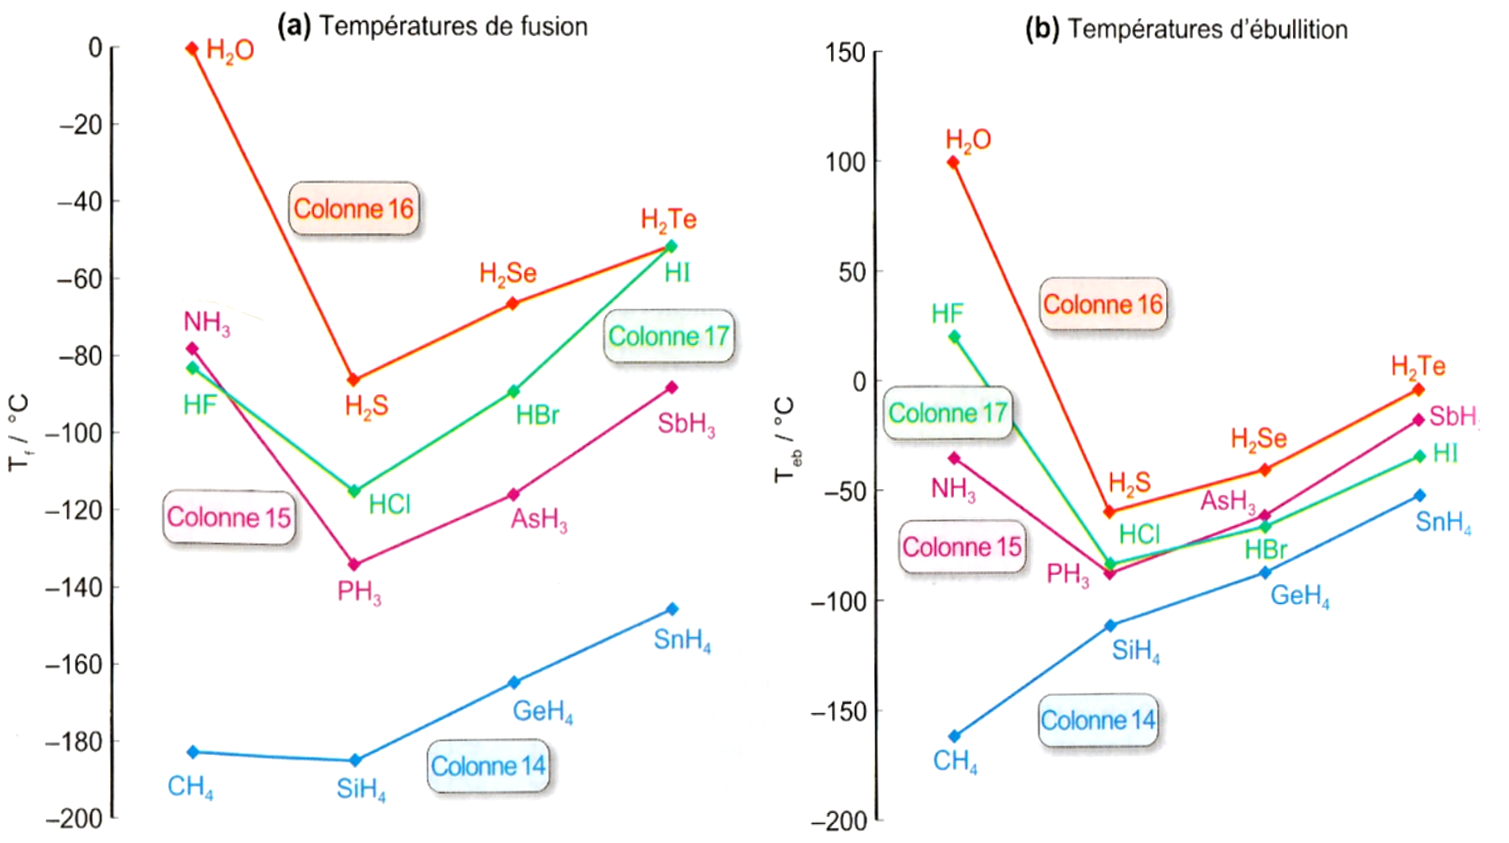
\includegraphics[width=.9\linewidth]{chimie/solvants/hydrures.png}
        \caption{Températures de fusion (a) et d'ébullition (b) des hydrures des éléments du bloc $p$ à pression atmosphérique.}
        \label{fig:hydrures}
    \end{figure}

\end{exercise}

\begin{exercise}{Nitrophénol$\cdot$s}{2}{PCSI}
{Atomistique,Classification périodique, Structure électronique}{bermu}

\begin{questions}
    \questioncours En introduisant dans le détail les concepts utilisés, commenter l'évolution des caractéristiques physiques des différents nitrophénols : ortho, méta et para.
 \end{questions}
 
\begin{table}[H]  
	\setchemfig{chemfig style={scale=0.75}, atom style={scale=0.75}}
    \begin{tabularx}{.8\linewidth}{r|CCC}
        & \chemfig{**6(---(-OH)-(-NO_3)---)}    %[scale=0.75][scale=0.75]
        & \chemfig{**6(--(-OH)--(-NO_3)---)}
        & \chemfig{**6(-(-OH)---(-NO_3)---)}\\
         & ortho & méta & para \\ \hline\hline
        Apparence & cristaux jaunes & cristaux incolores & aiguilles incolores \\
Point de fusion ($^\circ$C) & 44 & 97 & 114 \\
Point d'ébullition ($^\circ$C) & 214 & 194 & > 260 \\
pK$_a$ & 7,21 & 8,38 & 7,16 \\
Solubilité dans l'eau (g$\cdot$L$^{-1}$) & 2,1 & 13,5 & 14,8 \\ \hline
    \end{tabularx}

    \caption{Comparaisons de propriétés physiques des différents nitrophénols. (CTNP).}
\end{table}
\end{exercise}

\begin{exercise}{Catalyse par transfert de phase}{2}{MPSI}
{Atomistique,Classification périodique, Structure électronique}{bermu}

On s'intéresse à la réaction suivante entre les ions hypochlorite et l'alcool benzylique :
$$\mathrm{Ph-CH_2-OH + C\ell O^\ominus \quad\longrightarrow\quad Ph-CH=O + C\ell^\ominus + H_2O}$$

L'ion hypochlorite est dissout dans l'eau alors que l'acool est dissout dans un solvant organique : l'éthanoate d'étyle $\mathrm{CH_3-CO-O-CH_2-CH_3}$.

\begin{questions}
    \questioncours Rappeler le processus de solubilisation et justifier les deux solvants utilisés.
    
    \question En l'état, la réaction peut-elle se faire ? Pourquoi ne pas avoir utilisé un alcool comme milieu réactionnel ?
    
\uplevel{On introduit en petite quantités le sel TBAF de formule ionique $\mathrm{(C_4H_9)_4-N^\oplus + F^\ominus}$ .}
    
    \question Expliquer qu'après ajout de TBAF, la réaction à lieu.
    
\end{questions}

\end{exercise}

% Niveau :      PCSI *
% Discipline :  Chimie Orga I
% Mots clés :   Spectrométrie UV-visible, Réactions acidobasiques

\begin{exercise}{Chimie click, chimie verte}{2}{PCSI}
{Solvants}{bermu}



\begin{questions}
    \questioncours Différentes étapes de la solvatation d'un soluté dans un solvant. \\
    On illustrera la question d'exemple en rentrant dans le détail des différents types de solvants.

\begin{EnvUplevel}

Une des tendances actuelles en chimie de synthèse est la chimie click au micro-onde de la réaction de Biginelli :
\begin{center}
    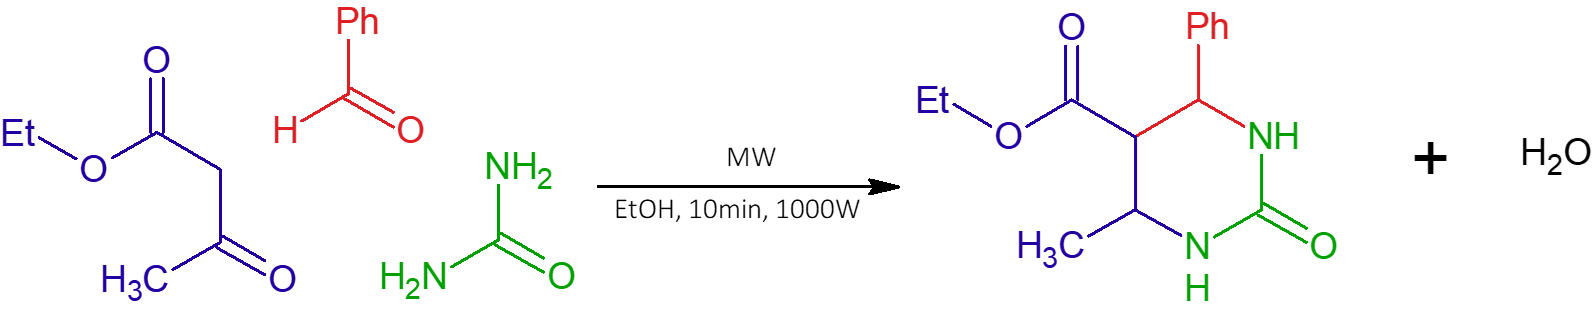
\includegraphics[width=.9\linewidth]{chimie/solvants/click.png}
\end{center}

\end{EnvUplevel}

    \question Justifier le choix de l'éthanol comme solvant de cette réaction.
    
\uplevel{Cette réaction  est activée grâce aux micro-ondes. Pour rappel, les fours à micro-ondes excitent à une fréquence spécifique pour exciter les molécules d'eau.}
    
    \question  Justifier que l'éthanol est excité par les micro-ondes et que cela permet de catalyser la réaction.
    
    \uplevel{Normalement, une telle réaction se ferait en plusieurs d'étapes dans plusieurs solvants.}
    
    \question Conclure quant aux gains écologique pour réaliser cette réaction. Pour information les 12 principes de la chimie verte ci-dessous.
    
    \begin{table}[H]
        \centering
        \begin{tabular}{ll}
            \\\hline\hline
            1. Prévention : moins de déchets ; &
            7. Matières renouvelables  ;\\
            2. Économie d'atomes : moins de sous-produits ; &
            8. Schéma de synthèse efficace ;\\
            3. Réactif doux : pas de substances toxiques ; &
            9. Catalyse ;\\
            4. Réduire la toxicité des produits utilisés ; &
            10. Produits biodégradables ;\\
            5. Pas de substances auxiliaires (solvants...) &
            11. Contrôle des conditions de réaction ; \\
            6. Conditions douces : CNTP ; &
            12. Réduire les risques d'accidents. \\ \hline
        \end{tabular}
        \caption{Principes de la chimie verte}
    \end{table}
\end{questions}
\end{exercise}

\section{Réactions de complexation (PC)}
% Niveau :      PCSI *
% Discipline :  Chimie Orga I
% Mots clés :   Spectrométrie UV-visible, Réactions acidobasiques

\begin{exercise}{\'Etude des thiocyanates}{2}{PCSI}
{Chimie générale,Réactions de complexation}{bermu}

\begin{questions}
\questioncours Structure et stabilité des complexes en solution aqueuse. \\ On définira les constantes de formation.

\begin{EnvUplevel}
    On s'intéresse à présent aux complexes formés par les ions thiocyanates SCN$^{-}$ et cuivre (II). Leur diagramme de distribution en fonction de pSCN $=-\log\dfrac{\mathrm{[SCN]}}{c^\circ}$ (où $c^\circ = 1$~M) est donné ci-dessous : \vspace{-.5em}
    
    \begin{figure}[H]
        \centering
        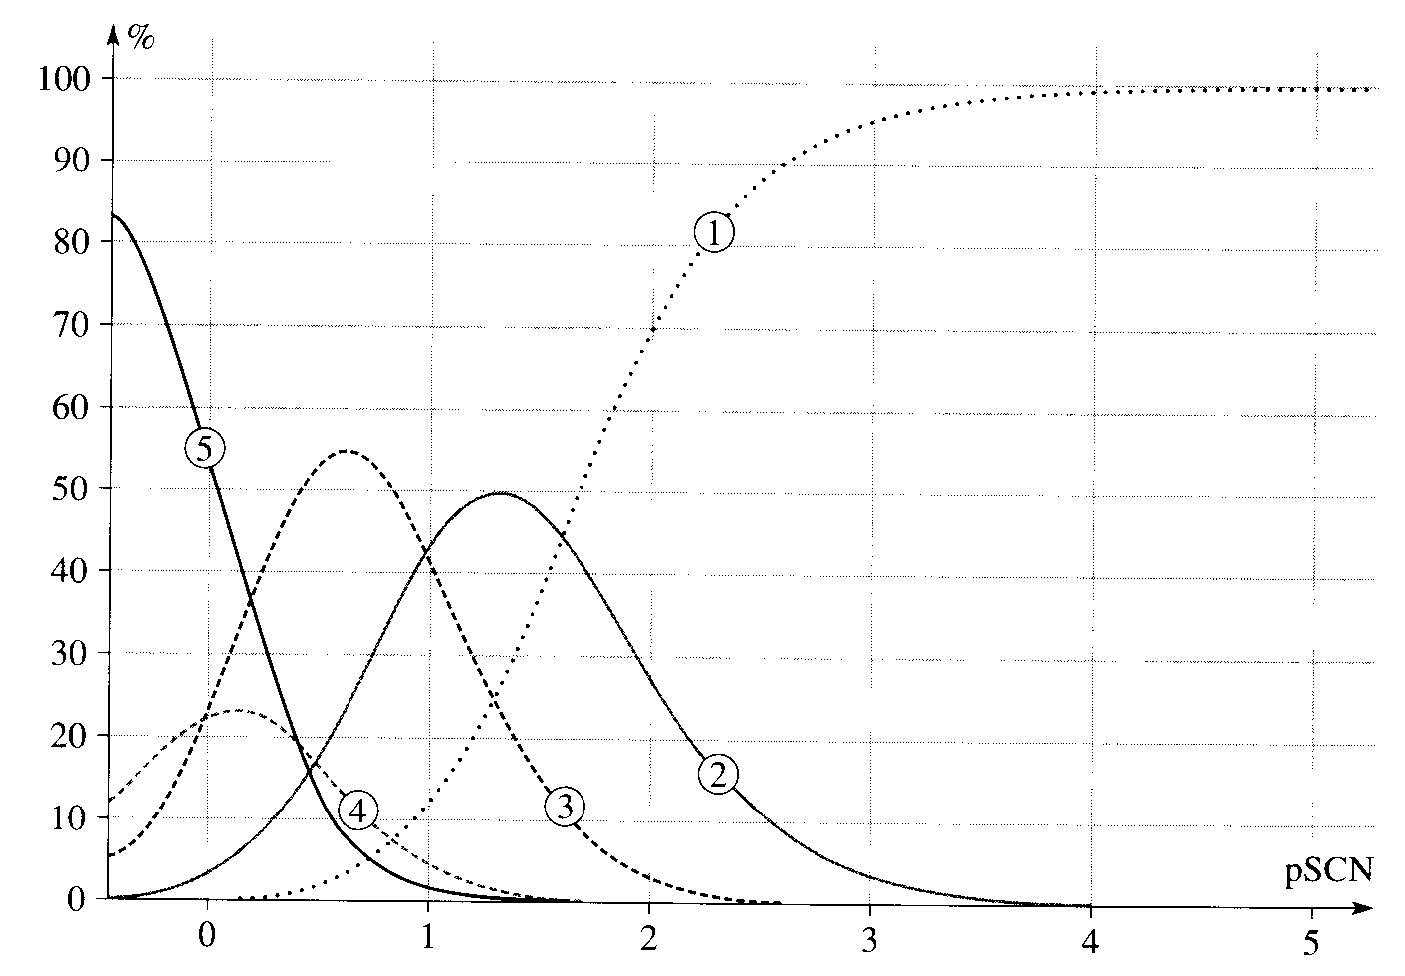
\includegraphics[width=.9\linewidth]{chimiePC/gene/thio.jpg}\vspace{-1.3em}
        \caption{Diagramme de distribution de complexes entre Cu$^{2+}$ et SCN$^{-}$.} \vspace{-0.8em}
    \end{figure}
\end{EnvUplevel}

\question Le numéro atomique du cuivre est $Z = 29$. En déduire la position de cet élément dans le tableau périodique (numéro de ligne, numéro de colonne) en justifiant la réponse. Donner la configuration électronique de l’ion Cu$^{2+}$.

\question Montrer que le ligand thiocyanate SCN$^{-}$ peut être écrit selon deux formes mésomères de représentativité proche. \\
Expliquer alors pourquoi on qualifie ce ligand de ligand ambidenté, et non pas de ligand bidenté.

\question Donner la formule et la nomenclature du complexe correspondant à chacune des courbes.

\question Déterminer les constantes de formation successives p$K_{fi}$ de ces complexes en justifiant la méthode utilisée.

\question Le complexe correspondant à la courbe 4 a une forte tendance à la dismutation. À quoi le voit-on sur le diagramme de distribution ? \\
Écrire l'équation chimique qui rende compte de ce phénomène et calculer sa constante d’équilibre. \\
Justifier rapidement que ce complexe soit peu stable comparé aux autres.

\begin{EnvUplevel}
    On constitue une solution aqueuse de 250 mL en dissolvant 10 mmol de sulfate de cuivre CuSO$_4$ et 1,0 mmol de thiocyanate de potassium KSCN.
\end{EnvUplevel}

\question{\sffamily Question ouverte :} En faisant les approximations nécessaires, donner les réactions chimiques qui ont lieu et décrire le système chimique à l'équilibre.

\end{questions}

\paragraph{Données : }~\\
L’indice de coordination du complexe Cu$^{2+}$ / SCN$^{-}$ varie de 1 à 4.

\end{exercise}

\begin{solution}

\begin{questions}
    \stepcounter{question}

    \question En appliquant les règles de remplissage :
    $$\mathrm{[Cu]} : 1s^2 2s^2 2p^6 3s^2 3p^6 4s^2 3d^9,$$
    {\sffamily Remarque :} dans le cas du cuivre, par la règle de Hund, il est plus facile d'avoir la configuration de valence $4s^1 3d^10$ car les énergies de la $4s$ et la $3d$ sont proches.
    
    Le cuivre est donc dans la 4ème période ($4s$) et le cuivre est dans la 11ème colonne $4s^2 3d^9$.
    
    $$\text{Ainsi la configuration de Cu}^{2+} \text{ est } \quad 1s^2 2s^2 2p^6 3s^2 3p^6 4s^0 3d^9.$$
    
    \question\hfill
    \schemestart
        \chemfig{@{a1}{^\ominus\hspace{1ex}\lewis{246,S}}-[@{a2},1.3]C~[@{b1},1.1]@{b2}\lewis{0,N}}
        \chemmove[red,-stealth,red,shorten >=3pt]{
            \draw(a1)..controls +(up:5mm) and +(north west:2mm).. (a2);}
        \chemmove[red,-stealth,red,shorten <=2pt]{
            \draw(b1)..controls +(up:5mm) and +(north west:2mm).. (b2);}
        \arrow{<->}[,1.5]
        \chemfig{\lewis{35,S}=[,1.1]C=[,1.3]\lewis{17,N}\hspace{1ex}^\ominus}
    \schemestop\chemnameinit{}\hfill~
    
    Le soufre et l’azote sont d’électronégativités voisines et donc ces deux formules mésomères sont de représentativités proches : la charge négative est à peu près équitablement répartie entre  N et S. L’ion SCN$^{-}$ peut donc se lier par S ou bien par N, mais pas simultanément puisque l’ion est linéaire (VSEPR AX$_2$), d'où la qualification d'ambidente.
    
    \question \`A haut pSCN (très bas [SCN]), il n'y a que Cu$^{2+}$, ainsi :
    \begin{enumerate}
        \item ~Cu$^{2+}$, ion cuivre II ;
        \item ~[CuSCN]$^+$, ion thiocyanatocuivre II ;
        \item ~[Cu(SCN)$_2$], dithiocyanatocuivre II ;
        \item ~[Cu(SCN)$_3$]$^{-}$, trithiocyanatocuprate II ;
        \item ~[Cu(SCN)$_4$]$^{2-}$, tetrathiocyanatocuprate II.
    \end{enumerate}
    
    \question p$K_{fi}$ est la constante de la réaction $[\mathrm{Cu(SCN)}_{i-1}]^{3-i} + \mathrm{[SCN^-]} \longrightarrow [\mathrm{Cu(SCN)}_i]^{2-i}$ donc
    $$\text{pSCN} = \log K_{fi} + \log\dfrac{[\mathrm{Cu(SCN)}_{i-1}]^{3-i}}{[\mathrm{Cu(SCN)}_i]^{2-i}}.$$
    \`A l'intersection des courbes $i$ et $i+1$, on a $[\mathrm{Cu(SCN)}_{i-1}]^{3-i} = [\mathrm{Cu(SCN)}_i]^{2-i}$ soit pSCN = $\log K_{fi}$.
    
    Donc $K_{f1} = 10^{1,6}$, $K_{f2} = 10^{1}$, $K_{f3} = 10^0$, $K_{f4} = 10^{0,4}$ (! intersection 4-5 !).
    
    \question La dismutation s'écrit $\mathrm{2[Cu(SCN)_3]^- \leftrightharpoons [Cu(SCN)_2] + [Cu(SCN)_4]^{2-}}$, de constante $K = \dfrac{K_{f4}}{K_{f3}} = 10^{0,4} > 1$ thermodynamiquement favorisée (on forme 4 et on détruit 3).
    
    Cela est dû au fait que la coordination $n=3$ n'est pas favorisée (cf. config électronique)
    
    \question [Cu$^2+$]$ = 40$ mM et [SCN$^-$]$ = 4,0$ mM, soit pSCN$ = 2,4$. Donc d'après le schéma les espèces prédominantes sont [Cu$^{2+}$] et [SCN$^-$] et la réaction prépondérante sera :
    \begin{center}\begin{tabularx}{9cm}{r|C|C|C}
&
\multicolumn{1}{|c!{\makebox[0pt]{+}}}{Cu$^{2+}$}
&
\multicolumn{1}{c!{\makebox[0pt]{$\leftrightharpoons$}}}{SCN$^-$}
&
[CuSCN]$^-$
\\
\hline\hline
Init. & $c_1$ & $c_2$ & 0 \\
Eq. & $c_1 - \xi$ & $c_2 - \xi$ & $\xi$
\end{tabularx}\end{center}
    $$\text{pour laquelle :}\qquad K_{f1} = \dfrac{\xi}{(c_1 - \xi)(c_2 - \xi)} \qquad \Longleftrightarrow \qquad \xi \simeq 2,2 \text{ mM}.$$
    
Ensuite pour les autres espèces, l'avancement des $fi$ sera négligeable et on aura pour $i > 1$, \vspace{-.8em}
$$[\mathrm{Cu(SCN)}_i]^{2-i} = K_{fi} [\mathrm{SCN}^{-1}] [\mathrm{Cu(SCN)}_{i-1}]^{3-i},$$
et donc, en définitive :
\begin{itemize}
    \item $[\mathrm{Cu}^{2+}] = 3,8 \times 10^{-2} \text{ M}$ ;
    \item $[\mathrm{SCN}^-] = 1,8 \times 10^{-3} \text{ M}$ ;
    \item $[\mathrm{CuSCN}^-] = 2,2 \times 10^{-3} \text{ M}$ ;
    \item $[\mathrm{Cu(SCN)}_2] = 3,6 \times 10^{-5} \text{ M}$ ;
    \item $[\mathrm{Cu(SCN)}_3]^- = 5,8 \times 10^{-8} \text{ M}$ ;
    \item $[\mathrm{Cu(SCN)}_4]^{2-} = 2,6 \times 10^{-10} \text{ M}$ ;
\end{itemize}
    
    
    
\end{questions}
\end{solution}
% Niveau :      PCSI *
% Discipline :  Chimie Orga I
% Mots clés :   Spectrométrie UV-visible, Réactions acidobasiques

\begin{exercise}{Dureté de l'eau}{2}{PCSI}
{Chimie générale,Réactions de complexation,Dosage,Titrage}{bermu}

\noindent\begin{minipage}{\linewidth}
\begin{wrapfigure}{R}{0.35\textwidth}
    \chemfig{N(-[4]-[-6]^\ominus OOC)(-[-4]-[-6]^\ominus OOC)-[0]-[-2]-[0]N(-[-2]-[0]COO^\ominus)(-[2]-[0]COO^\ominus)}
\end{wrapfigure}

\quad L'EDTA (strucutre ci-contre), noté Y$^{4-}$, est un ligand organique hexadentate très utilisé en chimie minérale pour doser les ions métalliques avec lesquels il a une très bonne affinité par chélation, notamment afin de mesurer la \emph{dureté de l'eau} (la concentration en minéraux de l'eau) par dosage complexométrique.
\end{minipage}

\begin{questions}
\questioncours Influence de la nature du ligand et du métal sur la stabilité du complexe~formé. \\
On prendra pour exemple les complexes EDTA-métal et on commentera la figure suivante : \vspace{-1em}

\begin{EnvUplevel}
    \begin{figure}[H]
        \centering
        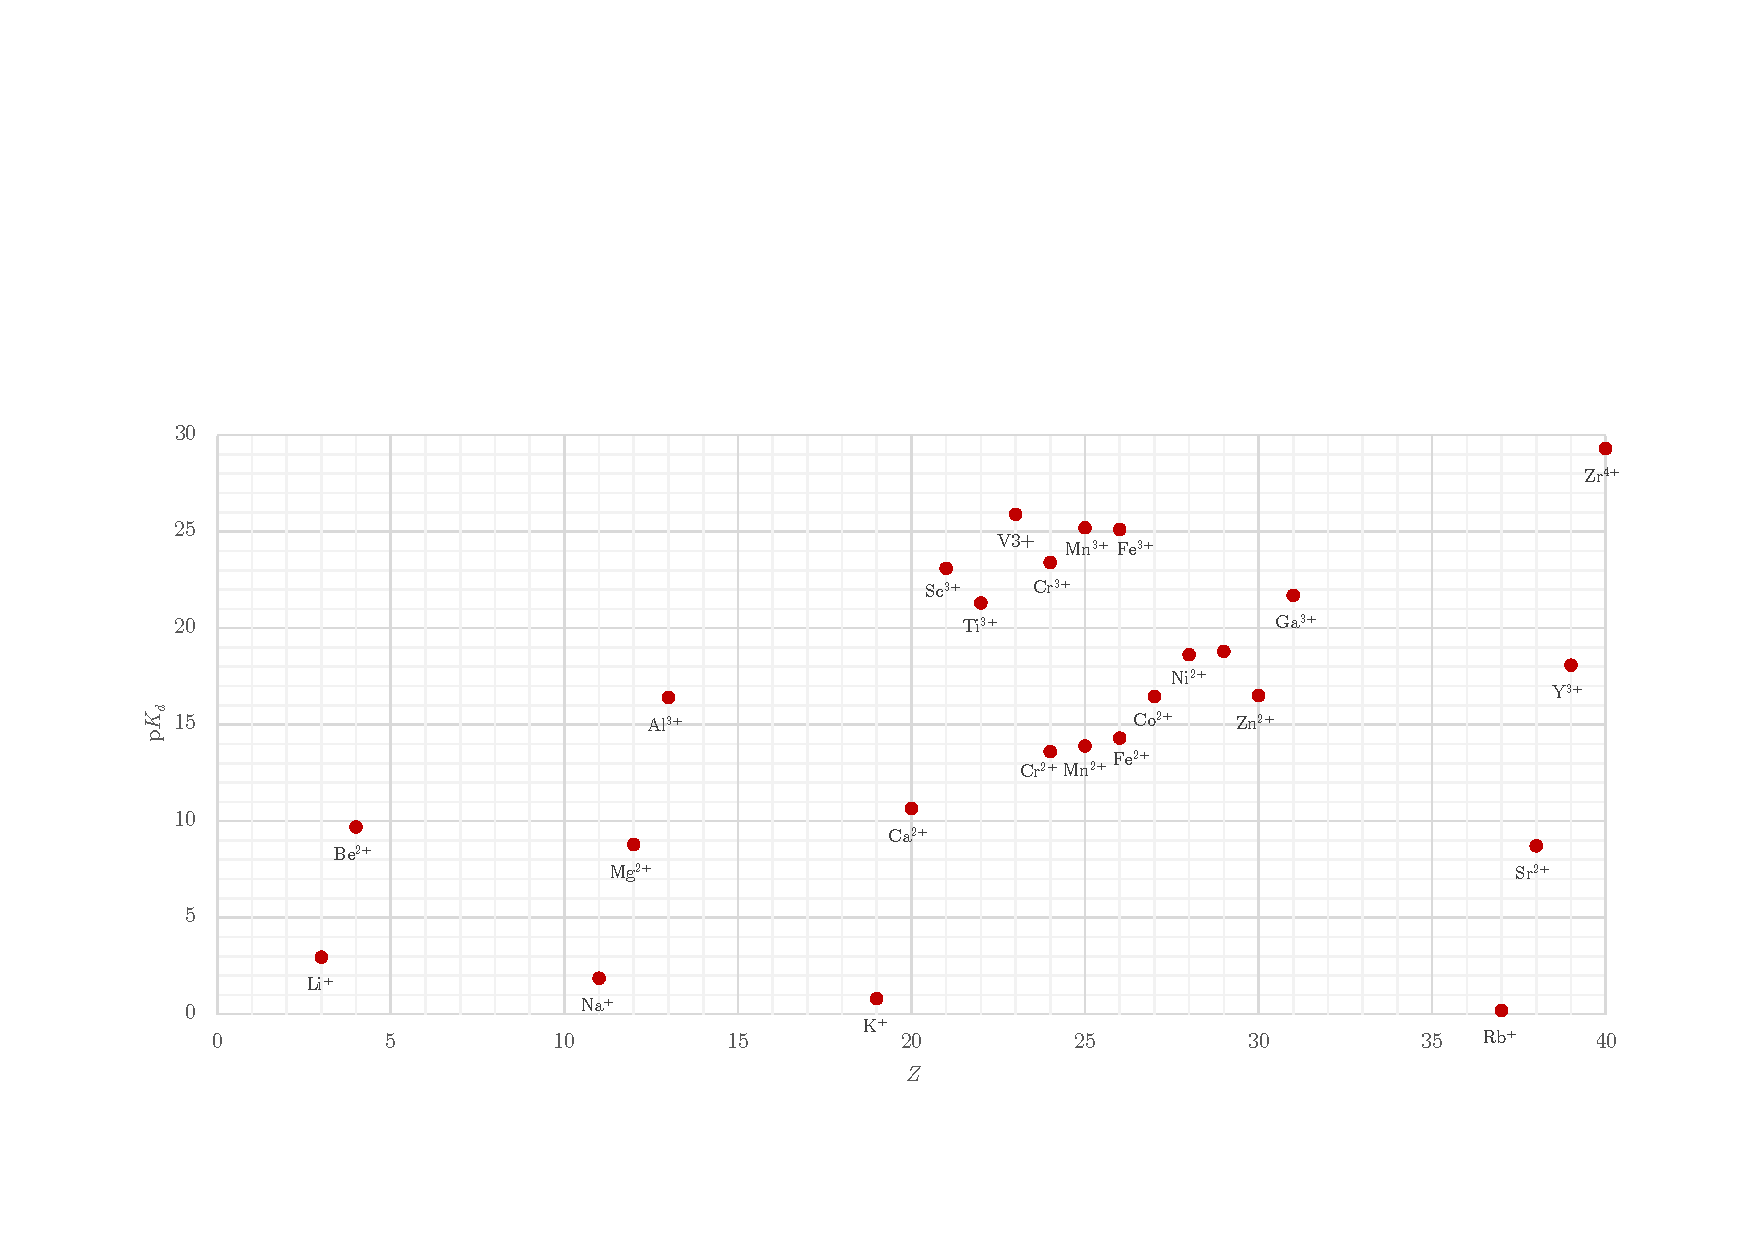
\includegraphics[width=\linewidth]{chimiePC/gene/EDTA.pdf}
        \caption{Constante de dissociation p$K_d$ des complexes métal-EDTA en fonction du numéro atomique $Z$ des ions métalliques.}
    \end{figure}
\end{EnvUplevel}

\question Repérer les sites ligands de Y$^{4-}$ et décrire la structure et la géométrie des complexes chélatés qu'il forme avec les ions métalliques.

\uplevel{On se propose de doser la dureté d'un volume $v_0$ d'eau du robinet avec une solution d'EDTA de concentration $c_1$. On note M$^{n+}$ les ions métalliques susceptibles de réagir.}

\question \'Ecrire la réaction du dosage et indiquer la constante de réaction. \\
Peut-on considérer que la réaction est totale ?

\question Donner la définition de l'équivalence et donner l'expression du volume équivalent $v_\text{eq}$.

\uplevel{Afin de détecter expérimentalement cette équivalence, les complexes d'EDTA étant incolores, on ajoute dans la solution avant le titrage quelques gouttes d'une solution de noir ériochrome T (NET) qui est noire sous sa forme déprotonée Net$^-$ et forme un complexe rouge avec les ions magnésium, calcium environ dix fois moins stables que ceux de l'EDTA.}

\question Décrire l'évolution de la couleur de la solution au cours du titrage.

\question Donner l'expression de la concentration $c_2$ en NET à apporter dans la solution initiale pour que le virage se produise à l’équivalence.

\question En quoi la précision du titrage serait-elle affectée si on introduisait au début du titrage une concentration 10 fois plus importante de NET ? 10 fois moins ? Commenter.

\question{\sffamily Question ouverte :} \'Etablir un protocole expérimental détaillé et chiffré pour mesurer la dureté de l'eau du robinet.

\end{questions}

\paragraph{Données : }~\\
La minéralisation typique de l'eau du robinet en alcalino-terreux est de 10 mg$\cdot$L$^{-1}$.

\noindent Masses molaires (g$\cdot$mol$^{-1}$) : Mg = 24, Ca = 40. 

\end{exercise}

\begin{solution}
\begin{questions}
    \questioncours Dans le cas particulier de l'EDTA, hexadentate :
    \begin{itemize}
        \item On remarque que les complexes des alcalins (colonne 1) sont moins stables que les complexes des alcalino-terreux (colonne 2) eux-mêmes moins stables que les complexes des métaux de transition des colonnes 3 et 4 :
        $$\mathrm{Li^+, Na^+, K^+, Rb^+ < Be^{2+}, Mg^{2+}, Ca^{2+}, Sr^{2+} < Al^{3+}, Sc^{3+}, Y^{3+} < Zr^{4+}.}$$
        
        Globalement, le complexe est plus stable avec des métaux présentant plus de trous dans leur couche de valence car ils forment plus de liaisons de coordination avec les différents sites de l'EDTA.
        
        \item Dans une même colonne, les complexes sont moins stables quand ils sont avec des métaux de rayon ionique élevé car les liaisons sont plus tendues :
        $$\mathrm{Li^+ > Na^+ > K^+ > Rb^+.}$$
        
        \item Pour les métaux de transition, une étude de leur configuration électronique permet de montrer que les plus stables sont ceux qui peuvent accepter 6 électrons en comblant leur couche de valence.
        
        \end{itemize}
    
    \question Les 6 sites ligands de Y$^{4-}$ sont les deux doublets non liants des deux azotes $\overline{\text{N}}$ et les 4 carboxylates COO$^\ominus$.
    
    Ils forment donc des complexes octaèdriques dans lesquels les métaux sont 'mis en cage' par l'EDTA, ce qui favorise grandement la stabilité du complexe.
    
    \question $\mathrm{Y^{4-} + M^{n+} \leftrightharpoons [YM]^{n-4}}$ de constante $1/K_d$ qui est de l'ordre de $10^9 \gg 1$ pour le magnésium : la réaction peut donc être considérée comme totale.
    
    \question L’équivalence est obtenue lorsqu’on a apporté Y$^{4-}$ et M$^{n+}$ dans les proportions st{\oe}chiométriques de la réaction de titrage, ici 1:1, soit
    $$n_\text{eq} = n_\mathrm{Y^{4-}} = n_\mathrm{M^{n+}} \qquad \Longleftrightarrow \qquad v_0 c_0 = c_1 v_\text{eq},$$
    en notant $c_0 = \mathrm{[M^{n+}]}_0$ la \emph{dureté} de l'eau.
    
    \question Au début, l'ion Net$^{-}$ se complexe immédiatement avec les ions métalliques M$^{n+}$ et forme un complexe rouge :
    $$\mathrm{Net^{-} + M^{n+} \longrightarrow MNet^{n-1}}\qquad\text{de constante } K_{d,\textsc{net}} \simeq 10 \times K_d.$$
    \`A l'équivalence, M$^{n+}$ est totalement consommé et la solution redevient noire.
    
    \question Le virage de l'indicateur se produit lorsque $\mathrm{[Net^{-}] \geqslant [MNet^{n-1}]}$, soit pour
    $$K_{d,\textsc{net}} = \mathrm{\dfrac{[Net^{-}][M^{n+}]}{[MNet^{n-1}]}} \geqslant \mathrm{[M^{n+}]_{eq}} \qqtext{soit} \mathrm{[M^{n+}]_{eq}} \leqslant 10^{-8}\text{ M},$$
    indépendemment de $c_2$.
    
    $c_2$ doit donc être simplement très petit devant $c_1$ pour ne pas perturber l'équivalence.
    
    %\`A l’équivalence le titrant a consommé exactement le titré : la réaction est quasi-totale. Il ne reste donc qu'une trace d'ions Y$^{4-}$ et M$^{n+}$, notée $\varepsilon$ telle que :
    %$$K_d = \mathrm{\dfrac{[M^{n+}][Y^{4-}]}{[MY^{n-4}]}} \simeq \dfrac{\varepsilon^2}{\frac{c_0 v_0}{v_0 + v_{eq}}} = \varepsilon^2 \dfrac{1 + c_1/c_0}{c_0} \qquad \Longleftrightarrow \varepsilon = \sqrt{\dfrac{K_d c_0}{1 + c_1/c_0}} \simeq 10^{-6} \text{ M},$$
    %en prenant $c_0 \simeq c_1 \simeq 1$ mM (cf. données) et $K_d \simeq 10^{-9}$.
    
    %Or 
    
    \question Si on apporte 10 plus de fois de NET, la réaction de complexation du NET, qui est quantitative, va déplacer l'équivalence vers de plus faibles volumes.
    
    En revanche, une plus petite concentration laisse inchangée l'équivalence : en revanche on risque de ne plus voir l'indicateur, ce qui serait dommage...
    
    \question{\sffamily Protocole : } d'après les données, $c_0 \simeq 1$ mM. Ainsi, il faut pour un $v_\text{eq} \simeq 20$ mL que $c_1 \simeq 5\times 10^{-4}$~M.
    
    Ensuite, on introduit dans un erlenmeyer $v_0 = 10$ mL d'eau du robinet à l'aide d'une pipette jaugée, une goutte de NET, on dilue jusqu'environ 100 mL pour le la dilution soit négligeable. Dans la burette on introduit une solution d'EDTA à $5\times 10^{-4}$ M préparée avec une fiole jaugée.
    
    \emph{ect.}
    
\end{questions}
\end{solution}
% Niveau :      PCSI *
% Discipline :  Chimie Orga I
% Mots clés :   Spectrométrie UV-visible, Réactions acidobasiques

\begin{exercise}{Influence du pH sur l'hémoglobine (2)}{2}{PCSI}
{Chimie générale,Réactions acidobasiques,Réactions de complexation}{bermu}

L'hémoglobine est une protéine globulaire qui permet de transporter le dioxygène $\mathrm{O_2}$ dans le sang des poumons vers les autres organes. Elle est constituée de 4 complexes du fer, appelés hèmes et notés $\mathrm{HmNH_2}$ qui se lient aux molécules de $\mathrm{O_2}$ dissoutes dans le sang.

Nous nous intéressons dans cet exercice à l'influence du pH sur la ligation du $\mathrm{O_2}$ sur les hèmes.

\begin{questions}
\questioncours Analogies et différences entre les réactions acido-basiques avec des polyacides AH$_n$ et les réactions de complexation avec des complexes ML$_n$. \\ On détaillera en particulier les considérations de stabilité (diagrammes de prédominance / distribution, $K_a$ / p$K_a$ et $K_d$ / p$K_d$).

\begin{EnvUplevel}
    Le mécanisme de complexation de l'hème avec le O$_2$ est le suivant :
    \begin{center}\schemestart[][-6]
        \chemfig{HmNH_2}
        \arrow{<=>[O$_{2\text{ (aq)}}$][$K_d$]}[0,1.5]
        \chemfig{O_2-HmNH_2}
        \arrow{<=>[H$^+_\text{ (aq)}$][?]}[-90,1.5]
        \chemfig{O_2-HmNH_3^+}
        \arrow{<=>[O$_{2\text{ (aq)}}$][$\gamma K_d$]}[-180,1.5]
        \chemfig{HmNH_3^+}
        \arrow{<=>[\rotatebox{180}{$K_a$}][\rotatebox{180}{H$^+_\text{ (aq)}$}]}[90,1.5]
    \schemestop\chemnameinit{}
    \end{center}
    
    $K_a = 2,6 \times 10^{-8}$ étant la constante d'acidité du groupe amine de l'hème, \\
    $K_d = 4,9 \times 10^{-6}$ la constante de dissociation de l'hème et du O$_2$, \\
    $\gamma = 0,73$ un facteur sans dimension.
\end{EnvUplevel}

\question Donner la relation entre le $K_d$ de l'hème et les concentrations des espèces en solution.

\question Donner la relation entre $K_a$, le pH et les concentrations des espèces en solutions.

\question Expliciter la constante de la réaction \chemfig{O_2-HmNH_2} $\leftrightharpoons$ \chemfig{O_2-HmNH_3^+}. \\
Quelle est la signification de $\gamma$ ?

\question Le pH favorise-t-il donc le transport du dioxygène dans le sang ?

\uplevel{On s'intéresse à la constante effective de dissociation $K_\text{eff}$ de l'hème qui prend en compte les formes acides et basiques de l'hème
$$K_\text{eff} = \mathrm{[O_2]} \times \dfrac{\Sigma \text{ espèces non liées}}{\Sigma \text{ espèces liées}}$$}

\question Expliciter l'expression de $K_\text{eff}$ en fonction des concentrations des espèces en solution puis en fonction uniquement du pH, $K_a$, $K_d$ et $\gamma$.

\uplevel{On appelle saturation S$_{\text{O}_2}$ la proportion de hèmes liés au dioxygène.}

\question Quel est le sens biologique de S$_{\text{O}_2}$ ?

\question Sachant que la concentration en $[\text{O}_2]$ est proportionnelle à la pression partielle $P_{\text{O}_2}$,\\
\hfill $[\text{O}_2] = \kappa_\textsc{h} P_{\text{O}_2},$ \hfill ~\\
montrer que S$_{\text{O}_2}$ peut s'écrire
$$\text{S}_{\text{O}_2} = \dfrac{P_{\text{O}_2}/P_{50}}{1 + P_{\text{O}_2}/P_{50}},$$
et expliciter l'expression et la signification de $P_{50}$.

\question{\sffamily Question ouverte :} Modéliser l'effet de ligands concurrents (CO$_2$, CN$^-$...) sur la S$_{\text{O}_2}$ et donner l'expression corrigée de la loi établie à la question précédente.

\end{questions}

\plusloin
Dash, R.K. \emph{et al, Ann Biomed Eng} \textbf{32}, 1676--1693 (2004).

\end{exercise}

\begin{solution}
\begin{questions}
    \questioncours
    \begin{itemize}
        \item Analogies : ces réactions de dissociation sont de manière générale
        $$\mathrm{XL_\textit{n} \leftrightharpoons X L_\textit{n-1} + L},$$
        et dont la constante est
        $$K_d = \mathrm{\dfrac{[XL_\textit{n-1}][L]}{[X L_\textit{n}]}} \quad \Longleftrightarrow \text{p}K_d = -\log K_d = \text{pL} + \log\mathrm{\dfrac{[XL_\textit{n-1}]}{[X L_\textit{n}]}}.$$
        \begin{center}\begin{tabular}{c|cc}
             & \textbf{Réactions acido-basiques} & \textbf{Réactions de coordination} \\ \hline\hline
            L & H$^+$ & Ligand \\
            XL$_n$ & Acide & Complexe \\
            XL$_{n-1}$ & Base & Complexe \\
        \end{tabular}\end{center}  
        
        \item La principale différence entre les réactions acide-base et de complexation est que les complexes peuvent dismuter ce qui n'est pas le cas pour les ampholytes car on a toujours
        $$\text{p}K_{a1} > \text{p}K_{a2} > \ldots,$$
        ce qui n'est pas le cas pour les complexes.
    \end{itemize}
    
    \question \hfill $K_d = \mathrm{\dfrac{[HmNH_2][O_2]}{[O_2\cdot HmNH_2]}}.$ \hfill ~
    
    \question Et de même \hfill $K_a = \mathrm{\dfrac{[HmNH_2][H^+]}{[HmNH_3^+]}}.$ \hfill ~
    
    \question La constante de la réaction $\mathrm{HmNH_2 \longrightarrow O_2\cdot HmNH_3^+}$ étant $\gamma K_a K_d$, la constante de la réaction $\mathrm{HmNH_3^+ \longrightarrow O_2\cdot HmNH_3^+}$ est $\gamma K_a$. \\
    $1/\gamma$ est donc le facteur indiquant à quel point la coordination du dioxygène O$_2$ par l'hème est moins efficace lorsque celle-ci est protonée.
    
    \question Et comme $\gamma < 1$, une augmentation de $\mathrm{[H^+]}$ / diminution de pH défavorise la coordination de O$_2$ par l'hème (souvent, H$^+$ défavorise les réactions de coordination).
    
    \question $K_\text{eff} = \mathrm{[O_2] \times \dfrac{[HmNH_2] + [HmNH_3^+]}{[O_2\cdot HmNH_2] + [O_2\cdot HmNH_3^+]}}
    = K_d \times \mathrm{\dfrac{[O_2\cdot HmNH_2] + \gamma [O_2\cdot HmNH_3^+]}{[O_2\cdot HmNH_2] + [O_2\cdot HmNH_3^+]}}$
    $$\text{d'où} \qquad K_\text{eff} = K_d \dfrac{1 + \dfrac{[H^+]}{K_a}}{1 + \dfrac{1}{\gamma}\,\dfrac{[H^+]}{K_a}}$$
    
    \question La S$_{\text{O}_2}$ représente la fraction d'hémoglobine qui transporte effectivement du O$_2$. C'est le marqueur biologique de l'efficacité de la respiration.
    
    \question $$\mathrm{S_{O_2}} = \dfrac{\mathrm{[O_2]}/K_\text{eff}}{1 + \mathrm{[O_2]}/K_\text{eff}} = \dfrac{P_{\text{O}_2}/P_{50}}{1 + P_{\text{O}_2}/P_{50}},$$
    avec $P_{50} = K_\text{eff} / \kappa_\textsc{h}$, la pression partielle en O$_2$ nécessaire à avoir une S$_{\text{O}_2}$ à 50\%.
    
    \question L'hème peut également complexer le CO$_2$ et CN$^-$ et va donc faire diminuer la S$_{\text{O}_2}$.
    
    Notons de manière générale L le ligand qui interfère et $K_\textsc{l}$ sa constante de dissociation, alors S$_{\text{O}_2}$ devient :
    $$\mathrm{S_{O_2}} = \dfrac{P_{\text{O}_2}/P_{50}}{1 + P_{\text{O}_2}/P_{50} + \mathrm{\dfrac{[L\cdot HmNH_2]}{[HmNH_2]}}} = \dfrac{P_{\text{O}_2}/P_{50}}{1 + P_{\text{O}_2}/P_{50} + \dfrac{a_\textsc{l}}{K_\textsc{l}}},$$
    $a_\textsc{l}$ étant l'activité de L en solution, $\mathrm{[CN^-]}$ pour le cynaure ou $P_\mathrm{CO_2}/\kappa_\mathrm{CO_2}$ pour le CO$_2$.
    
    On peut ensuite décliner un modèle analogue à celui de O$_2$ pour l'influence du pH sur la coordination de L.
\end{questions}
\end{solution}



